\usepackage[english]{babel}
\usepackage[T1]{fontenc}
\usepackage{graphicx}
\hyphenation{mo-no-poly car-ne-gie pro-ject pro-gress mo-dem rou-lette
  browse-wrap Use-net mon-as-tery mo-dems}
\hyphenation{co-me-dic polt-roon stove-pipe Ma-dame scru-ta-ble star-tling}
\hyphenation{heal-thily lim-ou-sines wrest-lers tan-trum push-over un-asked
  bras-siere bro-th-er}
\hyphenation{Can-a-da Fred-rick teen-agers wrest-ler Cha-vez Tho-mas 
  a-nom-a-lies sur-veil-lance ar-mies ref-u-gee ref-u-gees bris-tling
  eve-ning man-chu-ria man-chu-ri-an mid-terms me-di-um jap-a-nese}
\hyphenation{spend-ers googl-ing tour-ist tour-ists leg-end-ary}
\hyphenation{Dan-iel Van-essa Doc-to-row Ste-phen-son}
\hyphenation{de-cade sur-veilled rout-ers Wol-fen-stein teen-ager to-night}
\hyphenation{his-to-gram an-o-nym-ize Ga-la-xy sym-pa-the-tic}
\hyphenation{ar-phid ar-phids Found-ers}
\hyphenation{stran-ger stran-gers shoul-der-blades dump-ling dump-lings}
\hyphenation{ice-pack guard-rail Sep-tem-ber boot-able e-co-nom-ist}
\hyphenation{grown-ups roos-ter shoe-laces li-quid-i-ty}
\hyphenation{side-arm}
\hyphenation{wo-man wo-men tan-trum tan-trums Le-nin-grad zom-bie bunk-house}
\hyphenation{up-tick bio-mass}
\hyphenation{of-fi-cial of-fi-cial-ly gov-ern-ment}
\hyphenation{heal-thy Or-ville spark-ling}
\hyphenation{ves-ti-bule Law-rence au-to-no-mous}
\hyphenation{sau-sage door-step staf-fer}
\hyphenation{tree-trunk}
\hyphenation{to-ron-to}
\hyphenation{qua-dril-lion-aire qua-dril-lion-aires}
\hyphenation{sports-jack-et sports-jack-ets}
\hyphenation{work-space skunk-works}
\hyphenation{kings-ton}


\newcommand{\inlineimage}[1]{\raisebox{-0.4mm}{\includegraphics[scale=0.75]{#1}}}

\begin{document}
\raggedbottom
\thispagestyle{empty}
\begin{center}
    \huge{\textuppercase{THE NARRATIVE}}\\
    \vfill
    \normalsize{\textuppercase{OF}}\\
    \vfill
    \Huge{\textuppercase{ARTHUR GORDON PYM.}}\\
    \vfill
    \Large{\textuppercase{OF NANTUCKET.}}\\
    \vfill
    \normalsize{
    \textuppercase{COMPRISING THE DETAILS OF A MUTINY AND ATROCIOUS BUTCHERY.
    ON BOARD THE AMERICAN BRIG, GRAMPUS, ON HER WAY TO
    THE SOUTH SEAS, IN THE MONTH OF JUNE, 1827.}
    \medskip
    
    \textuppercase{WITH AN ACCOUNT OF THE RECAPTURE OF THE VESSEL BY THE
    SURVIVERS; THEIR SHIPWRECK AND SUBSEQUENT HORRIBLE
    SUFFERINGS FROM FAMINE; THEIR DELIVERANCE BY
    MEANS OF THE BRITISH SCHOONER JANE GUY; THE
    BRIEF CRUISE OF THIS LATTER VESSEL IN THE
    ANTARCTIC OCEAN; HER CAPTURE, AND THE
    MASSACRE OF HER CREW AMONG A
    GROUP OF ISLANDS IN THE}}\\
    \vfill
    \Large{\textuppercase{EIGHTY-FOURTH PARALLEL OF SOUTHERN LATITUDE;}}\\
    \vfill
    \normalsize{\textuppercase{TOGETHER WITH THE INCREDIBLE ADVENTURES AND
    DISCOVERIES}}\\
    \vfill
    \Large{\textuppercase{STILL FARTHER SOUTH}}\\
    \vfill
    \normalsize{\textuppercase{TO WHICH THAT DISTRESSING CALAMITY GAVE RISE.}}
\end{center}
\newpage
\section{Preface}
\textuppercase{UPON} my return to the United States a few months ago, after the extraordinary
series of adventure in the South Seas and elsewhere, of which an account is
given in the following pages, accident threw me into the society of several
gentlemen in Richmond, Va., who felt deep interest in all matters relating to
the regions I had visited, and who were constantly urging it upon me, as a duty,
to give my narrative to the public. I had several reasons, however, for
declining to do so, some of which were of a nature altogether private, and
concern no person but myself; others not so much so. One consideration which
deterred me was, that, having kept no journal during a greater portion of the
time in which I was absent, I feared I should not be able to write, from mere
memory, a statement so minute and connected as to have the \emph{appearance} of
that truth it would really possess, barring only the natural and unavoidable
exaggeration to which all of us are prone when detailing events which have had
powerful influence in exciting the imaginative faculties. Another reason was,
that the incidents to be narrated were of a nature so positively marvellous,
that, unsupported as my assertions must necessarily be (except by the evidence
of a single individual, and he a half-breed Indian), I could only hope for
belief among my family, and those of my friends who have had reason, through
life, to put faith in my veracity---the probability being that the public at
large would regard what I should put forth as merely an impudent and ingenious
fiction. A distrust in my own abilities as a writer was, nevertheless, one of
the principal causes which prevented me from complying with the suggestions of
my advisers. 

Among those gentlemen in Virginia who expressed the greatest interest in my
statement, more particularly in regard to that portion of it which related to
the Antarctic Ocean, was Mr. Poe, lately editor of the Southern Literary
Messenger, a monthly magazine, published by Mr. Thomas W. White, in the city of
Richmond. He strongly advised me, among others, to prepare at once a full
account of what I had seen and undergone, and trust to the shrewdness and common
sense of the public---insisting, with great plausibility, that however roughly,
as regards mere authorship, my book should be got up, its very uncouthness, if
there were any, would give it all the better chance of being received as
truth. 

Notwithstanding this representation, I did not make up my mind to do as he
suggested. He afterward proposed (finding that I would not stir in the matter)
that I should allow him to draw up, in his own words, a narrative of the earlier
portion of my adventures, from facts afforded by myself, publishing it in the
Southern Messenger \emph{under the garb of fiction}. To this, perceiving no
objection, I consented, stipulating only that my real name should be retained.
Two numbers of the pretended fiction appeared, consequently, in the Messenger
for January and February (1837), and, in order that it might certainly be
regarded as fiction, the name of Mr. Poe was affixed to the articles in the
table of contents of the magazine. 

The manner in which this \emph{ruse} was received has induced me at length to
undertake a regular compilation and publication of the adventures in question;
for I found that, in spite of the air of fable which had been so ingeniously
thrown around that portion of my statement which appeared in the Messenger
(without altering or distorting a single fact), the public were still not at all
disposed to receive it as fable, and several letters were sent to Mr. P.'s
address distinctly expressing a conviction to the contrary. I thence concluded
that the facts of my narrative would prove of such a nature as to carry with
them sufficient evidence of their own authenticity, and that I had consequently
little to fear on the score of popular incredulity. 

This \emph{exposé} being made, it will be seen at once how much of what
follows I claim to be my own writing; and it will also be understood that no
fact is misrepresented in the first few pages which were written by Mr. Poe.
Even to those readers who have not seen the Messenger, it will be unnecessary to
point out where his portion ends and my own commences; the difference in point
of style will be readily perceived. 

\section{Chapter 1}
My name is Arthur Gordon Pym. My father was a respectable trader in
sea-stores at Nantucket, where I was born. My maternal grandfather was an
attorney in good practice. He was fortunate in every thing, and had speculated
very successfully in stocks of the Edgarton New Bank, as it was formerly called.
By these and other means he had managed to lay by a tolerable sum of money. He
was more attached to myself, I believe, than to any other person in the world,
and I expected to inherit the most of his property at his death. He sent me, at
six years of age, to the school of old Mr. Ricketts, a gentleman with only one
arm and of eccentric manners---he is well known to almost every person who has
visited New Bedford. I stayed at his school until I was sixteen, when I left him
for Mr. E. Ronald's academy on the hill. Here I became intimate with the son of
Mr. Barnard, a sea-captain, who generally sailed in the employ of Lloyd and
Vredenburgh---Mr. Barnard is also very well known in New Bedford, and has many
relations, I am certain, in Edgarton. His son was named Augustus, and he was
nearly two years older than myself. He had been on a whaling voyage with his
father in the John Donaldson, and was always talking to me of his adventures in
the South Pacific Ocean. I used frequently to go home with him, and remain all
day, and sometimes all night. We occupied the same bed, and he would be sure to
keep me awake until almost light, telling me stories of the natives of the
Island of Tinian, and other places he had visited in his travels. At last I
could not help being interested in what he said, and by degrees I felt the
greatest desire to go to sea. I owned a sailboat called the Ariel, and worth
about seventy-five dollars. She had a half-deck or cuddy, and was rigged
sloop-fashion---I forget her tonnage, but she would hold ten persons without
much crowding. In this boat we were in the habit of going on some of the maddest
freaks in the world; and, when I now think of them, it appears to me a thousand
wonders that I am alive today. 

I will relate one of these adventures by way of introduction to a longer and
more momentous narrative. One night there was a party at Mr. Barnard's, and both
Augustus and myself were not a little intoxicated toward the close of it. As
usual, in such cases, I took part of his bed in preference to going home. He
went to sleep, as I thought, very quietly (it being near one when the party
broke up), and without saying a word on his favorite topic. It might have been
half an hour from the time of our getting in bed, and I was just about falling
into a doze, when he suddenly started up, and swore with a terrible oath that he
would not go to sleep for any Arthur Pym in Christendom, when there was so
glorious a breeze from the southwest. I never was so astonished in my life, not
knowing what he intended, and thinking that the wines and liquors he had drunk
had set him entirely beside himself. He proceeded to talk very coolly, however,
saying he knew that I supposed him intoxicated, but that he was never more sober
in his life. He was only tired, he added, of lying in bed on such a fine night
like a dog, and was determined to get up and dress, and go out on a frolic with
the boat. I can hardly tell what possessed me, but the words were no sooner out
of his mouth than I felt a thrill of the greatest excitement and pleasure, and
thought his mad idea one of the most delightful and most reasonable things in
the world. It was blowing almost a gale, and the weather was very cold---it
being late in October. I sprang out of bed, nevertheless, in a kind of ecstasy,
and told him I was quite as brave as himself, and quite as tired as he was of
lying in bed like a dog, and quite as ready for any fun or frolic as any
Augustus Barnard in Nantucket. 

We lost no time in getting on our clothes and hurrying down to the boat. She
was lying at the old decayed wharf by the lumber-yard of Pankey \& Co., and
almost thumping her side out against the rough logs. Augustus got into her and
bailed her, for she was nearly half full of water. This being done, we hoisted
jib and mainsail, kept full, and started boldly out to sea. 

The wind, as I before said, blew freshly from the southwest. The night was
very clear and cold. Augustus had taken the helm, and I stationed myself by the
mast, on the deck of the cuddy. We flew along at a great rate---neither of us
having said a word since casting loose from the wharf. I now asked my companion
what course he intended to steer, and what time he thought it probable we should
get back. He whistled for a few minutes, and then said crustily: ``\emph{I} am
going to sea---\emph{you} may go home if you think proper.'' Turning my eyes upon
him, I perceived at once that, in spite of his assumed \emph{nonchalance}, he
was greatly agitated. I could see him distinctly by the light of the moon---his
face was paler than any marble, and his hand shook so excessively that he could
scarcely retain hold of the tiller. I found that something had gone wrong, and
became seriously alarmed. At this period I knew little about the management of a
boat, and was now depending entirely upon the nautical skill of my friend. The
wind, too, had suddenly increased, as we were fast getting out of the lee of the
land---still I was ashamed to betray any trepidation, and for almost half an
hour maintained a resolute silence. I could stand it no longer, however, and
spoke to Augustus about the propriety of turning back. As before, it was nearly
a minute before he made answer, or took any notice of my suggestion.
``By-and-by,'' said he at length---``time enough---home by-and-by.'' I had expected
a similar reply, but there was something in the tone of these words which filled
me with an indescribable feeling of dread. I again looked at the speaker
attentively. His lips were perfectly livid, and his knees shook so violently
together that he seemed scarcely able to stand. ``For God's sake, Augustus,'' I
screamed, now heartily frightened, ``what ails you?---what is the matter?---what
\emph{are} you going to do?'' ``Matter!'' he stammered, in the greatest apparent
surprise, letting go the tiller at the same moment, and falling forward into the
bottom of the boat- ``matter---why, nothing is the---matter---going
home---d---d---don't you see?'' The whole truth now flashed upon me. I flew to
him and raised him up. He was drunk---beastly drunk---he could no longer either
stand, speak, or see. His eyes were perfectly glazed; and as I let him go in the
extremity of my despair, he rolled like a mere log into the bilge-water, from
which I had lifted him. It was evident that, during the evening, he had drunk
far more than I suspected, and that his conduct in bed had been the result of a
highly-concentrated state of intoxication---a state which, like madness,
frequently enables the victim to imitate the outward demeanour of one in perfect
possession of his senses. The coolness of the night air, however, had had its
usual effect---the mental energy began to yield before its influence---and the
confused perception which he no doubt then had of his perilous situation had
assisted in hastening the catastrophe. He was now thoroughly insensible, and
there was no probability that he would be otherwise for many hours. 

It is hardly possible to conceive the extremity of my terror. The fumes of
the wine lately taken had evaporated, leaving me doubly timid and irresolute. I
knew that I was altogether incapable of managing the boat, and that a fierce
wind and strong ebb tide were hurrying us to destruction. A storm was evidently
gathering behind us; we had neither compass nor provisions; and it was clear
that, if we held our present course, we should be out of sight of land before
daybreak. These thoughts, with a crowd of others equally fearful, flashed
through my mind with a bewildering rapidity, and for some moments paralyzed me
beyond the possibility of making any exertion. The boat was going through the
water at a terrible rate---full before the wind---no reef in either jib or
mainsail---running her bows completely under the foam. It was a thousand wonders
she did not broach to---Augustus having let go the tiller, as I said before, and
I being too much agitated to think of taking it myself. By good luck, however,
she kept steady, and gradually I recovered some degree of presence of mind.
Still the wind was increasing fearfully, and whenever we rose from a plunge
forward, the sea behind fell combing over our counter, and deluged us with
water. I was so utterly benumbed, too, in every limb, as to be nearly
unconscious of sensation. At length I summoned up the resolution of despair, and
rushing to the mainsail let it go by the run. As might have been expected, it
flew over the bows, and, getting drenched with water, carried away the mast
short off by the board. This latter accident alone saved me from instant
destruction. Under the jib only, I now boomed along before the wind, shipping
heavy seas occasionally over the counter, but relieved from the terror of
immediate death. I took the helm, and breathed with greater freedom as I found
that there yet remained to us a chance of ultimate escape. Augustus still lay
senseless in the bottom of the boat; and as there was imminent danger of his
drowning (the water being nearly a foot deep just where he fell), I contrived to
raise him partially up, and keep him in a sitting position, by passing a rope
round his waist, and lashing it to a ringbolt in the deck of the cuddy. Having
thus arranged every thing as well as I could in my chilled and agitated
condition, I recommended myself to God, and made up my mind to bear whatever
might happen with all the fortitude in my power. 

Hardly had I come to this resolution, when, suddenly, a loud and long scream
or yell, as if from the throats of a thousand demons, seemed to pervade the
whole atmosphere around and above the boat. Never while I live shall I forget
the intense agony of terror I experienced at that moment. My hair stood erect on
my head---I felt the blood congealing in my veins---my heart ceased utterly to
beat, and without having once raised my eyes to learn the source of my alarm, I
tumbled headlong and insensible upon the body of my fallen companion. 

I found myself, upon reviving, in the cabin of a large whaling-ship (the
Penguin) bound to Nantucket. Several persons were standing over me, and
Augustus, paler than death, was busily occupied in chafing my hands. Upon seeing
me open my eyes, his exclamations of gratitude and joy excited alternate
laughter and tears from the rough-looking personages who were present. The
mystery of our being in existence was now soon explained. We had been run down
by the whaling-ship, which was close-hauled, beating up to Nantucket with every
sail she could venture to set, and consequently running almost at right angles
to our own course. Several men were on the look-out forward, but did not
perceive our boat until it was an impossibility to avoid coming in contact-
their shouts of warning upon seeing us were what so terribly alarmed me. The
huge ship, I was told, rode immediately over us with as much ease as our own
little vessel would have passed over a feather, and without the least
perceptible impediment to her progress. Not a scream arose from the deck of the
victim---there was a slight grating sound to be heard mingling with the roar of
wind and water, as the frail bark which was swallowed up rubbed for a moment
along the keel of her destroyer---but this was all. Thinking our boat (which it
will be remembered was dismasted) some mere shell cut adrift as useless, the
captain (Captain E. T. V. Block, of New London) was for proceeding on his course
without troubling himself further about the matter. Luckily, there were two of
the look-out who swore positively to having seen some person at our helm, and
represented the possibility of yet saving him. A discussion ensued, when Block
grew angry, and, after a while, said that ``it was no business of his to be
eternally watching for egg-shells; that the ship should \emph{not} put about for
any such nonsense; and if there was a man run down, it was nobody's fault but
Henderson, the first mate, now took the matter up, being justly indignant, as
well as the whole ship's crew, at a speech evincing so base a degree of
heartless atrocity. He spoke plainly, seeing himself upheld by the men, told the
captain he considered him a fit subject for the gallows, and that he would
disobey his orders if he were hanged for it the moment he set his foot on shore.
He strode aft, jostling Block (who turned pale and made no answer) on one side,
and seizing the helm, gave the word, in a firm voice, \emph{Hard-a-lee!} The men
flew to their posts, and the ship went cleverly about. All this had occupied
nearly five minutes, and it was supposed to be hardly within the bounds of
possibility that any individual could be saved- allowing any to have been on
board the boat. Yet, as the reader has seen, both Augustus and myself were
rescued; and our deliverance seemed to have been brought about by two of those
almost inconceivable pieces of good fortune which are attributed by the wise and
pious to the special interference of Providence. 

While the ship was yet in stays, the mate lowered the jolly-boat and jumped
into her with the very two men, I believe, who spoke up as having seen me at the
helm. They had just left the lee of the vessel (the moon still shining brightly)
when she made a long and heavy roll to windward, and Henderson, at the same
moment, starting up in his seat bawled out to his crew to \emph{back water}. He
would say nothing else---repeating his cry impatiently, \emph{back water! black
water!} The men put back as speedily as possible, but by this time the ship
had gone round, and gotten fully under headway, although all hands on board were
making great exertions to take in sail. In despite of the danger of the attempt,
the mate clung to the main-chains as soon as they came within his reach. Another
huge lurch now brought the starboard side of the vessel out of water nearly as
far as her keel, when the cause of his anxiety was rendered obvious enough. The
body of a man was seen to be affixed in the most singular manner to the smooth
and shining bottom (the Penguin was coppered and copper-fastened), and beating
violently against it with every movement of the hull. After several ineffectual
efforts, made during the lurches of the ship, and at the imminent risk of
swamping the boat I was finally disengaged from my perilous situation and taken
on board- for the body proved to be my own. It appeared that one of the
timber-bolts having started and broken a passage through the copper, it had
arrested my progress as I passed under the ship, and fastened me in so
extraordinary a manner to her bottom. The head of the bolt had made its way
through the collar of the green baize jacket I had on, and through the back part
of my neck, forcing itself out between two sinews and just below the right ear.
I was immediately put to bed---although life seemed to be totally extinct. There
was no surgeon on board. The captain, however, treated me with every
attention---to make amends, I presume, in the eyes of his crew, for his
atrocious behaviour in the previous portion of the adventure. 

In the meantime, Henderson had again put off from the ship, although the wind
was now blowing almost a hurricane. He had not been gone many minutes when he
fell in with some fragments of our boat, and shortly afterward one of the men
with him asserted that he could distinguish a cry for help at intervals amid the
roaring of the tempest. This induced the hardy seamen to persevere in their
search for more than half an hour, although repeated signals to return were made
them by Captain Block, and although every moment on the water in so frail a boat
was fraught to them with the most imminent and deadly peril. Indeed, it is
nearly impossible to conceive how the small jolly they were in could have
escaped destruction for a single instant. She was built, however, for the
whaling service, and was fitted, as I have since had reason to believe, with
air-boxes, in the manner of some life-boats used on the coast of Wales. 

After searching in vain for about the period of time just mentioned, it was
determined to get back to the ship. They had scarcely made this resolve when a
feeble cry arose from a dark object that floated rapidly by. They pursued and
soon overtook it. It proved to be the entire deck of the Ariel's cuddy. Augustus
was struggling near it, apparently in the last agonies. Upon getting hold of him
it was found that he was attached by a rope to the floating timber. This rope,
it will be remembered, I had myself tied around his waist, and made fast to a
ringbolt, for the purpose of keeping him in an upright position, and my so
doing, it appeared, had been ultimately the means of preserving his life. The
Ariel was slightly put together, and in going down her frame naturally went to
pieces; the deck of the cuddy, as might have been expected, was lifted, by the
force of the water rushing in, entirely from the main timbers, and floated (with
other fragments, no doubt) to the surface- Augustus was buoyed up with it, and
thus escaped a terrible death. 

It was more than an hour after being taken on board the Penguin before he
could give any account of himself, or be made to comprehend the nature of the
accident which had befallen our boat. At length he became thoroughly aroused,
and spoke much of his sensations while in the water. Upon his first attaining
any degree of consciousness, he found himself beneath the surface, whirling
round and round with inconceivable rapidity, and with a rope wrapped in three or
four folds tightly about his neck. In an instant afterward he felt himself going
rapidly upward, when, his head striking violently against a hard substance, he
again relapsed into insensibility. Upon once more reviving he was in fuller
possession of his reason---this was still, however, in the greatest degree
clouded and confused. He now knew that some accident had occurred, and that he
was in the water, although his mouth was above the surface, and he could breathe
with some freedom. Possibly, at this period the deck was drifting rapidly before
the wind, and drawing him after it, as he floated upon his back. Of course, as
long as he could have retained this position, it would have been nearly
impossible that he should be drowned. Presently a surge threw him directly
athwart the deck, and this post he endeavored to maintain, screaming at
intervals for help. just before he was discovered by Mr. Henderson, he had been
obliged to relax his hold through exhaustion, and, falling into the sea, had
given himself up for lost. During the whole period of his struggles he had not
the faintest recollection of the Ariel, nor of the matters in connexion with the
source of his disaster. A vague feeling of terror and despair had taken entire
possession of his faculties. When he was finally picked up, every power of his
mind had failed him; and, as before said, it was nearly an hour after getting on
board the Penguin before he became fully aware of his condition. In regard to
myself---I was resuscitated from a state bordering very nearly upon death (and
after every other means had been tried in vain for three hours and a half) by
vigorous friction with flannels bathed in hot oil---a proceeding suggested by
Augustus. The wound in my neck, although of an ugly appearance, proved of little
real consequence, and I soon recovered from its effects. 

The Penguin got into port about nine o'clock in the morning, after
encountering one of the severest gales ever experienced off Nantucket. Both
Augustus and myself managed to appear at Mr. Barnard's in time for
breakfast---which, luckily, was somewhat late, owing to the party over night. I
suppose all at the table were too much fatigued themselves to notice our jaded
appearance- of course, it would not have borne a very rigid scrutiny.
Schoolboys, however, can accomplish wonders in the way of deception, and I
verily believe not one of our friends in Nantucket had the slightest suspicion
that the terrible story told by some sailors in town of their having run down a
vessel at sea and drowned some thirty or forty poor devils, had reference either
to the Ariel, my companion, or myself. We two have since very frequently talked
the matter over---but never without a shudder. In one of our conversations
Augustus frankly confessed to me, that in his whole life he had at no time
experienced so excruciating a sense of dismay, as when on board our little boat
he first discovered the extent of his intoxication, and felt himself sinking
beneath its influence. 

\section{Chapter 2}
In no affairs of mere prejudice, pro or con, do we deduce inferences with
entire certainty, even from the most simple data. It might be supposed that a
catastrophe such as I have just related would have effectually cooled my
incipient passion for the sea. On the contrary, I never experienced a more
ardent longing for the wild adventures incident to the life of a navigator than
within a week after our miraculous deliverance. This short period proved amply
long enough to erase from my memory the shadows, and bring out in vivid light
all the pleasurably exciting points of color, all the picturesqueness, of the
late perilous accident. My conversations with Augustus grew daily more frequent
and more intensely full of interest. He had a manner of relating his stories of
the ocean (more than one half of which I now suspect to have been sheer
fabrications) well adapted to have weight with one of my enthusiastic
temperament and somewhat gloomy although glowing imagination. It is strange,
too, that he most strongly enlisted my feelings in behalf of the life of a
seaman, when he depicted his more terrible moments of suffering and despair. For
the bright side of the painting I had a limited sympathy. My visions were of
shipwreck and famine; of death or captivity among barbarian hordes; of a
lifetime dragged out in sorrow and tears, upon some gray and desolate rock, in
an ocean unapproachable and unknown. Such visions or desires---for they amounted
to desires---are common, I have since been assured, to the whole numerous race
of the melancholy among men- at the time of which I speak I regarded them only
as prophetic glimpses of a destiny which I felt myself in a measure bound to
fulfil. Augustus thoroughly entered into my state of mind. It is probable,
indeed, that our intimate communion had resulted in a partial interchange of
character. About eighteen months after the period of the Ariel's disaster, the
firm of Lloyd and Vredenburgh (a house connected in some manner with the
Messieurs Enderby, I believe, of Liverpool) were engaged in repairing and
fitting out the brig Grampus for a whaling voyage. She was an old hulk, and
scarcely seaworthy when all was done to her that could be done. I hardly know
why she was chosen in preference to other good vessels belonging to the same
owners---but so it was. Mr. Barnard was appointed to command her, and Augustus
was going with him. While the brig was getting ready, he frequently urged upon
me the excellency of the opportunity now offered for indulging my desire of
travel. He found me by no means an unwilling listener---yet the matter could not
be so easily arranged. My father made no direct opposition; but my mother went
into hysterics at the bare mention of the design; and, more than all, my
grandfather, from whom I expected much, vowed to cut me off with a shilling if I
should ever broach the subject to him again. These difficulties, however, so far
from abating my desire, only added fuel to the flame. I determined to go at all
hazards; and, having made known my intentions to Augustus, we set about
arranging a plan by which it might be accomplished. In the meantime I forbore
speaking to any of my relations in regard to the voyage, and, as I busied myself
ostensibly with my usual studies, it was supposed that I had abandoned the
design. I have since frequently examined my conduct on this occasion with
sentiments of displeasure as well as of surprise. The intense hypocrisy I made
use of for the furtherance of my project---an hypocrisy pervading every word and
action of my life for so long a period of time---could only have been rendered
tolerable to myself by the wild and burning expectation with which I looked
forward to the fulfilment of my long-cherished visions of travel. 

In pursuance of my scheme of deception, I was necessarily obliged to leave
much to the management of Augustus, who was employed for the greater part of
every day on board the Grampus, attending to some arrangements for his father in
the cabin and cabin hold. At night, however, we were sure to have a conference
and talk over our hopes. After nearly a month passed in this manner, without our
hitting upon any plan we thought likely to succeed, he told me at last that he
had determined upon everything necessary. I had a relation living in New
Bedford, a Mr. Ross, at whose house I was in the habit of spending occasionally
two or three weeks at a time. The brig was to sail about the middle of June
(June, 1827), and it was agreed that, a day or two before her putting to sea, my
father was to receive a note, as usual, from Mr. Ross, asking me to come over
and spend a fortnight with Robert and Emmet (his sons). Augustus charged himself
with the inditing of this note and getting it delivered. Having set out as
supposed, for New Bedford, I was then to report myself to my companion, who
would contrive a hiding-place for me in the Grampus. This hiding-place, he
assured me, would be rendered sufficiently comfortable for a residence of many
days, during which I was not to make my appearance. When the brig had proceeded
so far on her course as to make any turning back a matter out of question, I
should then, he said, be formally installed in all the comforts of the cabin;
and as to his father, he would only laugh heartily at the joke. Vessels enough
would be met with by which a letter might be sent home explaining the adventure
to my parents. 

The middle of June at length arrived, and every thing had been matured. The
note was written and delivered, and on a Monday morning I left the house for the
New Bedford packet, as supposed. I went, however, straight to Augustus, who was
waiting for me at the corner of a street. It had been our original plan that I
should keep out of the way until dark, and then slip on board the brig; but, as
there was now a thick fog in our favor, it was agreed to lose no time in
secreting me. Augustus led the way to the wharf, and I followed at a little
distance, enveloped in a thick seaman's cloak, which he had brought with him, so
that my person might not be easily recognized. just as we turned the second
corner, after passing Mr. Edmund's well, who should appear, standing right in
front of me, and looking me full in the face, but old Mr. Peterson, my
grandfather. ``Why, bless my soul, Gordon,'' said he, after a long pause, ``why,
why,---\emph{whose} dirty cloak is that you have on?'' ``Sir!'' I replied,
assuming, as well as I could, in the exigency of the moment, an air of offended
surprise, and talking in the gruffest of all imaginable tones---``sir! you are a
sum'mat mistaken---my name, in the first place, bee'nt nothing at all like
Goddin, and I'd want you for to know better, you blackguard, than to call my new
obercoat a darty one.'' For my life I could hardly refrain from screaming with
laughter at the odd manner in which the old gentleman received this handsome
rebuke. He started back two or three steps, turned first pale and then
excessively red, threw up his spectacles, then, putting them down, ran full tilt
at me, with his umbrella uplifted. He stopped short, however, in his career, as
if struck with a sudden recollection; and presently, turning round, hobbled off
down the street, shaking all the while with rage, and muttering between his
teeth: ``Won't do---new glasses---thought it was Gordon---d--d good-for-nothing
salt water Long Tom.'' 

After this narrow escape we proceeded with greater caution, and arrived at
our point of destination in safety. There were only one or two of the hands on
board, and these were busy forward, doing something to the forecastle combings.
Captain Barnard, we knew very well, was engaged at Lloyd and Vredenburgh's, and
would remain there until late in the evening, so we had little to apprehend on
his account. Augustus went first up the vessel's side, and in a short while I
followed him, without being noticed by the men at work. We proceeded at once
into the cabin, and found no person there. It was fitted up in the most
comfortable style---a thing somewhat unusual in a whaling-vessel. There were
four very excellent staterooms, with wide and convenient berths. There was also
a large stove, I took notice, and a remarkably thick and valuable carpet
covering the floor of both the cabin and staterooms. The ceiling was full seven
feet high, and, in short, every thing appeared of a more roomy and agreeable
nature than I had anticipated. Augustus, however, would allow me but little time
for observation, insisting upon the necessity of my concealing myself as soon as
possible. He led the way into his own stateroom, which was on the starboard side
of the brig, and next to the bulkheads. Upon entering, he closed the door and
bolted it. I thought I had never seen a nicer little room than the one in which
I now found myself. It was about ten feet long, and had only one berth, which,
as I said before, was wide and convenient. In that portion of the closet nearest
the bulkheads there was a space of four feet square, containing a table, a
chair, and a set of hanging shelves full of books, chiefly books of voyages and
travels. There were many other little comforts in the room, among which I ought
not to forget a kind of safe or refrigerator, in which Augustus pointed out to
me a host of delicacies, both in the eating and drinking department. 

He now pressed with his knuckles upon a certain spot of the carpet in one
corner of the space just mentioned, letting me know that a portion of the
flooring, about sixteen inches square, had been neatly cut out and again
adjusted. As he pressed, this portion rose up at one end sufficiently to allow
the passage of his finger beneath. In this manner he raised the mouth of the
trap (to which the carpet was still fastened by tacks), and I found that it led
into the after hold. He next lit a small taper by means of a phosphorous match,
and, placing the light in a dark lantern, descended with it through the opening,
bidding me follow. I did so, and he then pulled the cover upon the hole, by
means of a nail driven into the under side---the carpet, of course, resuming its
original position on the floor of the stateroom, and all traces of the aperture
being concealed. 

The taper gave out so feeble a ray that it was with the greatest difficulty I
could grope my way through the confused mass of lumber among which I now found
myself. By degrees, however, my eyes became accustomed to the gloom, and I
proceeded with less trouble, holding on to the skirts of my friend's coat. He
brought me, at length, after creeping and winding through innumerable narrow
passages, to an iron-bound box, such as is used sometimes for packing fine
earthenware. It was nearly four feet high, and full six long, but very narrow.
Two large empty oil-casks lay on the top of it, and above these, again, a vast
quantity of straw matting, piled up as high as the floor of the cabin. In every
other direction around was wedged as closely as possible, even up to the
ceiling, a complete chaos of almost every species of ship-furniture, together
with a heterogeneous medley of crates, hampers, barrels, and bales, so that it
seemed a matter no less than miraculous that we had discovered any passage at
all to the box. I afterward found that Augustus had purposely arranged the
stowage in this hold with a view to affording me a thorough concealment, having
had only one assistant in the labour, a man not going out in the brig. 

My companion now showed me that one of the ends of the box could be removed
at pleasure. He slipped it aside and displayed the interior, at which I was
excessively amused. A mattress from one of the cabin berths covered the whole of
its bottom, and it contained almost every article of mere comfort which could be
crowded into so small a space, allowing me, at the same time, sufficient room
for my accommodation, either in a sitting position or lying at full length.
Among other things, there were some books, pen, ink, and paper, three blankets,
a large jug full of water, a keg of sea-biscuit, three or four immense Bologna
sausages, an enormous ham, a cold leg of roast mutton, and half a dozen bottles
of cordials and liqueurs. I proceeded immediately to take possession of my
little apartment, and this with feelings of higher satisfaction, I am sure, than
any monarch ever experienced upon entering a new palace. Augustus now pointed
out to me the method of fastening the open end of the box, and then, holding the
taper close to the deck, showed me a piece of dark whipcord lying along it.
This, he said, extended from my hiding-place throughout an the necessary
windings among the lumber, to a nail which was driven into the deck of the hold,
immediately beneath the trap-door leading into his stateroom. By means of this
cord I should be enabled readily to trace my way out without his guidance,
provided any unlooked-for accident should render such a step necessary. He now
took his departure, leaving with me the lantern, together with a copious supply
of tapers and phosphorous, and promising to pay me a visit as often as he could
contrive to do so without observation. This was on the seventeenth of June. 

I remained three days and nights (as nearly as I could guess) in my
hiding-place without getting out of it at all, except twice for the purpose of
stretching my limbs by standing erect between two crates just opposite the
opening. During the whole period I saw nothing of Augustus; but this occasioned
me little uneasiness, as I knew the brig was expected to put to sea every hour,
and in the bustle he would not easily find opportunities of coming down to me.
At length I heard the trap open and shut. and presently he called in a low
voice, asking if all was well, and if there was any thing I wanted. ``Nothing,'' I
replied; ``I am as comfortable as can be; when will the brig sail?'' ``She will be
under weigh in less than half an hour,'' he answered. ``I came to let you know,
and for fear you should be uneasy at my absence. I shall not have a chance of
coming down again for some time---perhaps for three or four days more. All is
going on right aboveboard. After I go up and close the trap, do you creep along
by the whipcord to where the nail is driven in. You will find my watch
there---it may be useful to you, as you have no daylight to keep time by. I
suppose you can't tell how long you have been buried---only three days---this is
the twentieth. I would bring the watch to your box, but am afraid of being
missed.'' With this he went up. 

In about an hour after he had gone I distinctly felt the brig in motion, and
congratulated myself upon having at length fairly commenced a voyage. Satisfied
with this idea, I determined to make my mind as easy as possible, and await the
course of events until I should be permitted to exchange the box for the more
roomy, although hardly more comfortable, accommodations of the cabin. My first
care was to get the watch. Leaving the taper burning, I groped along in the
dark, following the cord through windings innumerable, in some of which I
discovered that, after toiling a long distance, I was brought back within a foot
or two of a former position. At length I reached the nail, and securing the
object of my journey, returned with it in safety. I now looked over the books
which had been so thoughtfully provided, and selected the expedition of Lewis
and Clarke to the mouth of the Columbia. With this I amused myself for some
time, when, growing sleepy, I extinguished the light with great care, and soon
fell into a sound slumber. 

Upon awakening I felt strangely confused in mind, and some time elapsed
before I could bring to recollection all the various circumstances of my
situation. By degrees, however, I remembered all. Striking a light, I looked at
the watch; but it was run down, and there were, consequently, no means of
determining how long I slept. My limbs were greatly cramped, and I was forced to
relieve them by standing between the crates. Presently feeling an almost
ravenous appetite, I bethought myself of the cold mutton, some of which I had
eaten just before going to sleep, and found excellent. What was my astonishment
in discovering it to be in a state of absolute putrefaction! This circumstance
occasioned me great disquietude; for, connecting it with the disorder of mind I
experienced upon awakening, I began to suppose that I must have slept for an
inordinately long period of time. The close atmosphere of the hold might have
had something to do with this, and might, in the end, be productive of the most
serious results. My head ached excessively; I fancied that I drew every breath
with difficulty; and, in short, I was oppressed with a multitude of gloomy
feelings. Still I could not venture to make any disturbance by opening the trap
or otherwise, and, having wound up the watch, contented myself as well as
possible. 

Throughout the whole of the next tedious twenty-four hours no person came to
my relief, and I could not help accusing Augustus of the grossest inattention.
What alarmed me chiefly was, that the water in my jug was reduced to about half
a pint, and I was suffering much from thirst, having eaten freely of the Bologna
sausages after the loss of my mutton. I became very uneasy, and could no longer
take any interest in my books. I was overpowered, too, with a desire to sleep,
yet trembled at the thought of indulging it, lest there might exist some
pernicious influence, like that of burning charcoal, in the confined air of the
hold. In the meantime the roll of the brig told me that we were far in the main
ocean, and a dull humming sound, which reached my ears as if from an immense
distance, convinced me no ordinary gale was blowing. I could not imagine a
reason for the absence of Augustus. We were surely far enough advanced on our
voyage to allow of my going up. Some accident might have happened to him---but I
could think of none which would account for his suffering me to remain so long a
prisoner, except, indeed, his having suddenly died or fallen overboard, and upon
this idea I could not dwell with any degree of patience. It was possible that we
had been baffled by head winds, and were still in the near vicinity of
Nantucket. This notion, however, I was forced to abandon; for such being the
case, the brig must have frequently gone about; and I was entirely satisfied,
from her continual inclination to the larboard, that she had been sailing all
along with a steady breeze on her starboard quarter. Besides, granting that we
were still in the neighborhood of the island, why should not Augustus have
visited me and informed me of the circumstance? Pondering in this manner upon
the difficulties of my solitary and cheerless condition, I resolved to wait yet
another twenty-four hours, when, if no relief were obtained, I would make my way
to the trap, and endeavour either to hold a parley with my friend, or get at
least a little fresh air through the opening, and a further supply of water from
the stateroom. While occupied with this thought, however, I fell in spite of
every exertion to the contrary, into a state of profound sleep, or rather
stupor. My dreams were of the most terrific description. Every species of
calamity and horror befell me. Among other miseries I was smothered to death
between huge pillows, by demons of the most ghastly and ferocious aspect.
Immense serpents held me in their embrace, and looked earnestly in my face with
their fearfully shining eyes. Then deserts, limitless, and of the most forlorn
and awe-inspiring character, spread themselves out before me. Immensely tall
trunks of trees, gray and leafless, rose up in endless succession as far as the
eye could reach. Their roots were concealed in wide-spreading morasses, whose
dreary water lay intensely black, still, and altogether terrible, beneath. And
the strange trees seemed endowed with a human vitality, and waving to and fro
their skeleton arms, were crying to the silent waters for mercy, in the shrill
and piercing accents of the most acute agony and despair. The scene changed; and
I stood, naked and alone, amidst the burning sand-plains of Sahara. At my feet
lay crouched a fierce lion of the tropics. Suddenly his wild eyes opened and
fell upon me. With a conculsive bound he sprang to his feet, and laid bare his
horrible teeth. In another instant there burst from his red throat a roar like
the thunder of the firmament, and I fell impetuously to the earth. Stifling in a
paroxysm of terror, I at last found myself partially awake. My dream, then, was
not all a dream. Now, at least, I was in possession of my senses. The paws of
some huge and real monster were pressing heavily upon my bosom---his hot breath
was in my ear---and his white and ghastly fangs were gleaming upon me through
the gloom. 

Had a thousand lives hung upon the movement of a limb or the utterance of a
syllable, I could have neither stirred nor spoken. The beast, whatever it was,
retained his position without attempting any immediate violence, while I lay in
an utterly helpless, and, I fancied, a dying condition beneath him. I felt that
my powers of body and mind were fast leaving me---in a word, that I was
perishing, and perishing of sheer fright. My brain swam---I grew deadly
sick---my vision failed---even the glaring eyeballs above me grew dim. Making a
last strong effort, I at length breathed a faint ejaculation to God, and
resigned myself to die. The sound of my voice seemed to arouse all the latent
fury of the animal. He precipitated himself at full length upon my body; but
what was my astonishment, when, with a long and low whine, he commenced licking
my face and hands with the greatest eagerness, and with the most extravagant
demonstration of affection and joy! I was bewildered, utterly lost in
amazement---but I could not forget the peculiar whine of my Newfoundland dog
Tiger, and the odd manner of his caresses I well knew. It was he. I experienced
a sudden rush of blood to my temples- a giddy and overpowering sense of
deliverance and reanimation. I rose hurriedly from the mattress upon which I had
been lying, and, throwing myself upon the neck of my faithful follower and
friend, relieved the long oppression of my bosom in a flood of the most
passionate tears. 

As upon a former occasion my conceptions were in a state of the greatest
indistinctness and confusion after leaving the mattress. For a long time I found
it nearly impossible to connect any ideas; but, by very slow degrees, my
thinking faculties returned, and I again called to memory the several incidents
of my condition. For the presence of Tiger I tried in vain to account; and after
busying myself with a thousand different conjectures respecting him, was forced
to content myself with rejoicing that he was with me to share my dreary
solitude, and render me comfort by his caresses. Most people love their
dogs---but for Tiger I had an affection far more ardent than common; and never,
certainly, did any creature more truly deserve it. For seven years he had been
my inseparable companion, and in a multitude of instances had given evidence of
all the noble qualities for which we value the animal. I had rescued him, when a
puppy, from the clutches of a malignant little villain in Nantucket who was
leading him, with a rope around his neck, to the water; and the grown dog repaid
the obligation, about three years afterward, by saving me from the bludgeon of a
street robber. 

Getting now hold of the watch, I found, upon applying it to my ear, that it
had again run down; but at this I was not at all surprised, being convinced,
from the peculiar state of my feelings, that I had slept, as before, for a very
long period of time, how long, it was of course impossible to say. I was burning
up with fever, and my thirst was almost intolerable. I felt about the box for my
little remaining supply of water, for I had no light, the taper having burnt to
the socket of the lantern, and the phosphorus-box not coming readily to hand.
Upon finding the jug, however, I discovered it to be empty---Tiger, no doubt,
having been tempted to drink it, as well as to devour the remnant of mutton, the
bone of which lay, well picked, by the opening of the box. The spoiled meat I
could well spare, but my heart sank as I thought of the water. I was feeble in
the extreme---so much so that I shook all over, as with an ague, at the
slightest movement or exertion. To add to my troubles, the brig was pitching and
rolling with great violence, and the oil-casks which lay upon my box were in
momentary danger of falling down, so as to block up the only way of ingress or
egress. I felt, also, terrible sufferings from sea-sickness. These
considerations determined me to make my way, at all hazards, to the trap, and
obtain immediate relief, before I should be incapacitated from doing so
altogether. Having come to this resolve, I again felt about for the
phosphorus-box and tapers. The former I found after some little trouble; but,
not discovering the tapers as soon as I had expected (for I remembered very
nearly the spot in which I had placed them), I gave up the search for the
present, and bidding Tiger lie quiet, began at once my journey toward the
trap. 

In this attempt my great feebleness became more than ever apparent. It was
with the utmost difficulty I could crawl along at all, and very frequently my
limbs sank suddenly from beneath me; when, falling prostrate on my face, I would
remain for some minutes in a state bordering on insensibility. Still I struggled
forward by slow degrees, dreading every moment that I should swoon amid the
narrow and intricate windings of the lumber, in which event I had nothing but
death to expect as the result. At length, upon making a push forward with all
the energy I could command, I struck my forehead violently against the sharp
corner of an iron-bound crate. The accident only stunned me for a few moments;
but I found, to my inexpressible grief, that the quick and violent roll of the
vessel had thrown the crate entirely across my path, so as effectually to block
up the passage. With my utmost exertions I could not move it a single inch from
its position, it being closely wedged in among the surrounding boxes and
ship-furniture. It became necessary, therefore, enfeebled as I was, either to
leave the guidance of the whipcord and seek out a new passage, or to climb over
the obstacle, and resume the path on the other side. The former alternative
presented too many difficulties and dangers to be thought of without a shudder.
In my present weak state of both mind and body, I should infallibly lose my way
if I attempted it, and perish miserably amid the dismal and disgusting
labyrinths of the hold. I proceeded, therefore, without hesitation, to summon up
all my remaining strength and fortitude, and endeavour, as I best might, to
clamber over the crate. 

Upon standing erect, with this end in view, I found the undertaking even a
more serious task than my fears had led me to imagine. On each side of the
narrow passage arose a complete wall of various heavy lumber, which the least
blunder on my part might be the means of bringing down upon my head; or, if this
accident did not occur, the path might be effectually blocked up against my
return by the descending mass, as it was in front by the obstacle there. The
crate itself was a long and unwieldy box, upon which no foothold could be
obtained. In vain I attempted, by every means in my power, to reach the top,
with the hope of being thus enabled to draw myself up. Had I succeeded in
reaching it, it is certain that my strength would have proved utterly inadequate
to the task of getting over, and it was better in every respect that I failed.
At length, in a desperate effort to force the crate from its ground, I felt a
strong vibration in the side next me. I thrust my hand eagerly to the edge of
the planks, and found that a very large one was loose. With my pocket-knife,
which, luckily, I had with me, I succeeded, after great labour, in prying it
entirely off; and getting it through the aperture, discovered, to my exceeding
joy, that there were no boards on the opposite side---in other words, that the
top was wanting, it being the bottom through which I had forced my way. I now
met with no important difficulty in proceeding along the line until I finally
reached the nail. With a beating heart I stood erect, and with a gentle touch
pressed against the cover of the trap. It did not rise as soon as I had
expected, and I pressed it with somewhat more determination, still dreading lest
some other person than Augustus might be in his state-room. The door, however,
to my astonishment, remained steady, and I became somewhat uneasy, for I knew
that it had formerly required but little or no effort to remove it. I pushed it
strongly---it was nevertheless firm: with all my strength---it still did not
give way: with rage, with fury, with despair---it set at defiance my utmost
efforts; and it was evident, from the unyielding nature of the resistance, that
the hole had either been discovered and effectually nailed up, or that some
immense weight had been placed upon it, which it was useless to think of
removing. 

My sensations were those of extreme horror and dismay. In vain I attempted to
reason on the probable cause of my being thus entombed. I could summon up no
connected chain of reflection, and, sinking on the floor, gave way,
unresistingly, to the most gloomy imaginings, in which the dreadful deaths of
thirst, famine, suffocation, and premature interment crowded upon me as the
prominent disasters to be encountered. At length there returned to me some
portion of presence of mind. I arose, and felt with my fingers for the seams or
cracks of the aperture. Having found them, I examined them closely to ascertain
if they emitted any light from the state-room; but none was visible. I then
forced the blade of my pen-knife through them, until I met with some hard
obstacle. Scraping against it, I discovered it to be a solid mass of iron,
which, from its peculiar wavy feel as I passed the blade along it, I concluded
to be a chain-cable. The only course now left me was to retrace my way to the
box, and there either yield to my sad fate, or try so to tranquilize my mind as
to admit of my arranging some plan of escape. I immediately set about the
attempt, and succeeded, after innumerable difficulties, in getting back. As I
sank, utterly exhausted, upon the mattress, Tiger threw himself at full length
by my side, and seemed as if desirous, by his caresses, of consoling me in my
troubles, and urging me to bear them with fortitude. 

The singularity of his behavior at length forcibly arrested my attention.
After licking my face and hands for some minutes, he would suddenly cease doing
so, and utter a low whine. Upon reaching out my hand toward him, I then
invariably found him lying on his back, with his paws uplifted. This conduct, so
frequently repeated, appeared strange, and I could in no manner account for it.
As the dog seemed distressed, I concluded that he had received some injury; and,
taking his paws in my hands, I examined them one by one, but found no sign of
any hurt. I then supposed him hungry, and gave him a large piece of ham, which
he devoured with avidity---afterward, however, resuming his extraordinary
manoeuvres. I now imagined that he was suffering, like myself, the torments of
thirst, and was about adopting this conclusion as the true one, when the idea
occurred to me that I had as yet only examined his paws, and that there might
possibly be a wound upon some portion of his body or head. The latter I felt
carefully over, but found nothing. On passing my hand, however, along his back,
I perceived a slight erection of the hair extending completely across it.
Probing this with my finger, I discovered a string, and tracing it up, found
that it encircled the whole body. Upon a closer scrutiny, I came across a small
slip of what had the feeling of letter paper, through which the string had been
fastened in such a manner as to bring it immediately beneath the left shoulder
of the animal. 

\section{Chapter 3}
The thought instantly occurred to me that the paper was a note from Augustus,
and that some unaccountable accident having happened to prevent his relieving me
from my dungeon, he had devised this method of acquainting me with the true
state of affairs. Trembling with eagerness, I now commenced another search for
my phosphorus matches and tapers. I had a confused recollection of having put
them carefully away just before falling asleep; and, indeed, previously to my
last journey to the trap, I had been able to remember the exact spot where I had
deposited them. But now I endeavored in vain to call it to mind, and busied
myself for a full hour in a fruitless and vexatious search for the missing
articles; never, surely, was there a more tantalizing state of anxiety and
suspense. At length, while groping about, with my head close to the ballast,
near the opening of the box, and outside of it, I perceived a faint glimmering
of light in the direction of the steerage. Greatly surprised, I endeavored to
make my way toward it, as it appeared to be but a few feet from my position.
Scarcely had I moved with this intention, when I lost sight of the glimmer
entirely, and, before I could bring it into view again, was obliged to feel
along by the box until I had exactly resumed my original situation. Now, moving
my head with caution to and fro, I found that, by proceeding slowly, with great
care, in an opposite direction to that in which I had at first started, I was
enabled to draw near the light, still keeping it in view. Presently I came
directly upon it (having squeezed my way through innumerable narrow windings),
and found that it proceeded from some fragments of my matches lying in an empty
barrel turned upon its side. I was wondering how they came in such a place, when
my hand fell upon two or three pieces of taper wax, which had been evidently
mumbled by the dog. I concluded at once that he had devoured the whole of my
supply of candles, and I felt hopeless of being ever able to read the note of
Augustus. The small remnants of the wax were so mashed up among other rubbish in
the barrel, that I despaired of deriving any service from them, and left them as
they were. The phosphorus, of which there was only a speck or two, I gathered up
as well as I could, and returned with it, after much difficulty, to my box,
where Tiger had all the while remained. 

What to do next I could not tell. The hold was so intensely dark that I could
not see my hand, however close I would hold it to my face. The white slip of
paper could barely be discerned, and not even that when I looked at it directly;
by turning the exterior portions of the retina toward it- that is to say, by
surveying it slightly askance, I found that it became in some measure
perceptible. Thus the gloom of my prison may be imagined, and the note of my
friend, if indeed it were a note from him, seemed only likely to throw me into
further trouble, by disquieting to no purpose my already enfeebled and agitated
mind. In vain I revolved in my brain a multitude of absurd expedients for
procuring light- such expedients precisely as a man in the perturbed sleep
occasioned by opium would be apt to fall upon for a similar purpose- each and
all of which appear by turns to the dreamer the most reasonable and the most
preposterous of conceptions, just as the reasoning or imaginative faculties
flicker, alternately, one above the other. At last an idea occurred to me which
seemed rational, and which gave me cause to wonder, very justly, that I had not
entertained it before. I placed the slip of paper on the back of a book, and,
collecting the fragments of the phosphorus matches which I had brought from the
barrel, laid them together upon the paper. I then, with the palm of my hand,
rubbed the whole over quickly, yet steadily. A clear light diffused itself
immediately throughout the whole surface; and had there been any writing upon
it, I should not have experienced the least difficulty, I am sure, in reading
it. Not a syllable was there, however---nothing but a dreary and unsatisfactory
blank; the illumination died away in a few seconds, and my heart died away
within me as it went. 

I have before stated more than once that my intellect, for some period prior
to this, had been in a condition nearly bordering on idiocy. There were, to be
sure, momentary intervals of perfect sanity, and, now and then, even of energy;
but these were few. It must be remembered that I had been, for many days
certainly, inhaling the almost pestilential atmosphere of a close hold in a
whaling vessel, and for a long portion of that time but scantily supplied with
water. For the last fourteen or fifteen hours I had none---nor had I slept
during that time. Salt provisions of the most exciting kind had been my chief,
and, indeed, since the loss of the mutton, my only supply of food, with the
exception of the sea-biscuit; and these latter were utterly useless to me, as
they were too dry and hard to be swallowed in the swollen and parched condition
of my throat. I was now in a high state of fever, and in every respect
exceedingly ill. This will account for the fact that many miserable hours of
despondency elapsed after my last adventure with the phosphorus, before the
thought suggested itself that I had examined only one side of the paper. I shall
not attempt to describe my feelings of rage (for I believe I was more angry than
any thing else) when the egregious oversight I had committed flashed suddenly
upon my perception. The blunder itself would have been unimportant, had not my
own folly and impetuosity rendered it otherwise---in my disappointment at not
finding some words upon the slip, I had childishly torn it in pieces and thrown
it away, it was impossible to say where. 

From the worst part of this dilemma I was relieved by the sagacity of Tiger.
Having got, after a long search, a small piece of the note, I put it to the
dog's nose, and endeavored to make him understand that he must bring me the rest
of it. To my astonishment, (for I had taught him none of the usual tricks for
which his breed are famous,) he seemed to enter at once into my meaning, and,
rummaging about for a few moments, soon found another considerable portion.
Bringing me this, he paused awhile, and, rubbing his nose against my hand,
appeared to be waiting for my approval of what he had done. I patted him on the
head, when he immediately made off again. It was now some minutes before he came
back- but when he did come, he brought with him a large slip, which proved to be
all the paper missing---it having been torn, it seems, only into three pieces.
Luckily, I had no trouble in finding what few fragments of the phosphorus were
left---being guided by the indistinct glow one or two of the particles still
emitted. My difficulties had taught me the necessity of caution, and I now took
time to reflect upon what I was about to do. It was very probable, I considered,
that some words were written upon that side of the paper which had not been
examined---but which side was that? Fitting the pieces together gave me no clew
in this respect, although it assured me that the words (if there were any) would
be found all on one side, and connected in a proper manner, as written. There
was the greater necessity of ascertaining the point in question beyond a doubt,
as the phosphorus remaining would be altogether insufficient for a third
attempt, should I fail in the one I was now about to make. I placed the paper on
a book as before, and sat for some minutes thoughtfully revolving the matter
over in my mind. At last I thought it barely possible that the written side
might have some unevenness on its surface, which a delicate sense of feeling
might enable me to detect. I determined to make the experiment and passed my
finger very carefully over the side which first presented itself. Nothing,
however, was perceptible, and I turned the paper, adjusting it on the book. I
now again carried my forefinger cautiously along, when I was aware of an
exceedingly slight, but still discernable glow, which followed as it proceeded.
This, I knew, must arise from some very minute remaining particles of the
phosphorus with which I had covered the paper in my previous attempt. The other,
or under side, then, was that on which lay the writing, if writing there should
finally prove to be. Again I turned the note, and went to work as I had
previously done. Having rubbed in the phosphorus, a brilliancy ensued as before-
but this time several lines of MS. in a large hand, and apparently in red ink,
became distinctly visible. The glimmer, although sufficiently bright, was but
momentary. Still, had I not been too greatly excited, there would have been
ample time enough for me to peruse the whole three sentences before me---for I
saw there were three. In my anxiety, however, to read all at once, I succeeded
only in reading the seven concluding words, which thus
appeared---``\emph{blood---your life depends upon lying close}.'' 

Had I been able to ascertain the entire contents of the note---the full
meaning of the admonition which my friend had thus attempted to convey, that
admonition, even although it should have revealed a story of disaster the most
unspeakable, could not, I am firmly convinced, have imbued my mind with one
tithe of the harrowing and yet indefinable horror with which I was inspired by
the fragmentary warning thus received. And ``\emph{blood},'' too, that word of all
words---so rife at all times with mystery, and suffering, and terror---how
trebly full of import did it now appear- how chilly and heavily (disjointed, as
it thus was, from any foregoing words to qualify or render it distinct) did its
vague syllables fall, amid the deep gloom of my prison, into the innermost
recesses of my soul! 

Augustus had, undoubtedly, good reasons for wishing me to remain concealed,
and I formed a thousand surmises as to what they could be---but I could think of
nothing affording a satisfactory solution of the mystery. Just after returning
from my last journey to the trap, and before my attention had been otherwise
directed by the singular conduct of Tiger, I had come to the resolution of
making myself heard at all events by those on board, or, if I could not succeed
in this directly, of trying to cut my way through the orlop deck. The half
certainty which I felt of being able to accomplish one of these two purposes in
the last emergency, had given me courage (which I should not otherwise have had)
to endure the evils of my situation. The few words I had been able to read,
however, had cut me off from these final resources, and I now, for the first
time, felt all the misery of my fate. In a paroxysm of despair I threw myself
again upon the mattress, where, for about the period of a day and night, I lay
in a kind of stupor, relieved only by momentary intervals of reason and
recollection. 

At length I once more arose, and busied myself in reflection upon the horrors
which encompassed me. For another twenty-four hours it was barely possible that
I might exist without water---for a longer time I could not do so. During the
first portion of my imprisonment I had made free use of the cordials with which
Augustus had supplied me, but they only served to excite fever, without in the
least degree assuaging thirst. I had now only about a gill left, and this was of
a species of strong peach liqueur at which my stomach revolted. The sausages
were entirely consumed; of the ham nothing remained but a small piece of the
skin; and all the biscuit, except a few fragments of one, had been eaten by
Tiger. To add to my troubles, I found that my headache was increasing
momentarily, and with it the species of delirium which had distressed me more or
less since my first falling asleep. For some hours past it had been with the
greatest difficulty I could breathe at all, and now each attempt at so doing was
attended with the most depressing spasmodic action of the chest. But there was
still another and very different source of disquietude, and one, indeed, whose
harassing terrors had been the chief means of arousing me to exertion from my
stupor on the mattress. It arose from the demeanor of the dog. 

I first observed an alteration in his conduct while rubbing in the phosphorus
on the paper in my last attempt. As I rubbed, he ran his nose against my hand
with a slight snarl; but I was too greatly excited at the time to pay much
attention to the circumstance. Soon afterward, it will be remembered, I threw
myself on the mattress, and fell into a species of lethargy. Presently I became
aware of a singular hissing sound close at my ears, and discovered it to proceed
from Tiger, who was panting and wheezing in a state of the greatest apparent
excitement, his eyeballs flashing fiercely through the gloom. I spoke to him,
when he replied with a low growl, and then remained quiet. Presently I relapsed
into my stupor, from which I was again awakened in a similar manner. This was
repeated three or four times, until finally his behaviour inspired me with so
great a degree of fear, that I became fully aroused. He was now lying close by
the door of the box, snarling fearfully, although in a kind of undertone, and
grinding his teeth as if strongly convulsed. I had no doubt whatever that the
want of water or the confined atmosphere of the hold had driven him mad, and I
was at a loss what course to pursue. I could not endure the thought of killing
him, yet it seemed absolutely necessary for my own safety. I could distinctly
perceive his eyes fastened upon me with an expression of the most deadly
animosity, and I expected every instant that he would attack me. At last I could
endure my terrible situation no longer, and determined to make my way from the
box at all hazards, and dispatch him, if his opposition should render it
necessary for me to do so. To get out, I had to pass directly over his body, and
he already seemed to anticipate my design---missing himself upon his forelegs
(as I perceived by the altered position of his eyes), and displayed the whole of
his white fangs, which were easily discernible. I took the remains of the
ham-skin, and the bottle containing the liqueur, and secured them about my
person, together with a large carving-knife which Augustus had left me---then,
folding my cloak around me as closely as possible, I made a movement toward the
mouth of the box. No sooner did I do this, than the dog sprang with a loud growl
toward my throat. The whole weight of his body struck me on the right shoulder,
and I fell violently to the left, while the enraged animal passed entirely over
me. I had fallen upon my knees, with my head buried among the blankets, and
these protected me from a second furious assault, during which I felt the sharp
teeth pressing vigorously upon the woollen which enveloped my neck- yet,
luckily, without being able to penetrate all the folds. I was now beneath the
dog, and a few moments would place me completely in his power. Despair gave me
strength, and I rose boldly up, shaking him from me by main force, and dragging
with me the blankets from the mattress. These I now threw over him, and before
he could extricate himself, I had got through the door and closed it effectually
against his pursuit. In this struggle, however, I had been forced to drop the
morsel of ham-skin, and I now found my whole stock of provisions reduced to a
single gill of liqueur, As this reflection crossed my mind, I felt myself
actuated by one of those fits of perverseness which might be supposed to
influence a spoiled child in similar circumstances, and, raising the bottle to
my lips, I drained it to the last drop, and dashed it furiously upon the
floor. 

Scarcely had the echo of the crash died away, when I heard my name pronounced
in an eager but subdued voice, issuing from the direction of the steerage. So
unexpected was anything of the kind, and so intense was the emotion excited
within me by the sound, that I endeavoured in vain to reply. My powers of speech
totally failed, and in an agony of terror lest my friend should conclude me
dead, and return without attempting to reach me, I stood up between the crates
near the door of the box, trembling convulsively, and gasping and struggling for
utterance. Had a thousand words depended upon a syllable, I could not have
spoken it. There was a slight movement now audible among the lumber somewhere
forward of my station. The sound presently grew less distinct, then again less
so, and still less. Shall I ever forget my feelings at this moment? He was
going---my friend, my companion, from whom I had a right to expect so much---he
was going---he would abandon me---he was gone! He would leave me to perish
miserably, to expire in the most horrible and loathesome of dungeons---and one
word, one little syllable, would save me---yet that single syllable I could not
utter! I felt, I am sure, more than ten thousand times the agonies of death
itself. My brain reeled, and I fell, deadly sick, against the end of the
box. 

As I fell the carving-knife was shaken out from the waist-band of my
pantaloons, and dropped with a rattling sound to the floor. Never did any strain
of the richest melody come so sweetly to my ears! With the intensest anxiety I
listened to ascertain the effect of the noise upon Augustus- for I knew that the
person who called my name could be no one but himself. All was silent for some
moments. At length I again heard the word ``\emph{Arthur!}'' repeated in a low
tone, and one full of hesitation. Reviving hope loosened at once my powers of
speech, and I now screamed at the top of my voice, ``\emph{Augustus! oh,
Augustus!}'' ``Hush! for God's sake be silent!'' he replied, in a voice
trembling with agitation; ``I will be with you immediately---as soon as I can
make my way through the hold.'' For a long time I heard him moving among the
lumber, and every moment seemed to me an age. At length I felt his hand upon my
shoulder, and he placed, at the same moment, a bottle of water to my lips. Those
only who have been suddenly redeemed from the jaws of the tomb, or who have
known the insufferable torments of thirst under circumstances as aggravated as
those which encompassed me in my dreary prison, can form any idea of the
unutterable transports which that one long draught of the richest of all
physical luxuries afforded. 

When I had in some degree satisfied my thirst, Augustus produced from his
pocket three or four boiled potatoes, which I devoured with the greatest
avidity. He had brought with him a light in a dark lantern, and the grateful
rays afforded me scarcely less comfort than the food and drink. But I was
impatient to learn the cause of his protracted absence, and he proceeded to
recount what had happened on board during my incarceration. 

\section{Chapter 4}
The brig put to sea, as I had supposed, in about an hour after he had left
the watch. This was on the twentieth of June. It will be remembered that I had
then been in the hold for three days; and, during this period, there was so
constant a bustle on board, and so much running to and fro, especially in the
cabin and staterooms, that he had had no chance of visiting me without the risk
of having the secret of the trap discovered. When at length he did come, I had
assured him that I was doing as well as possible; and, therefore, for the two
next days be felt but little uneasiness on my account---still, however, watching
an opportunity of going down. It was not \emph{until the fourth day} that he
found one. Several times during this interval he had made up his mind to let his
father know of the adventure, and have me come up at once; but we were still
within reaching distance of Nantucket, and it was doubtful, from some
expressions which had escaped Captain Barnard, whether he would not immediately
put back if he discovered me to be on board. Besides, upon thinking the matter
over, Augustus, so he told me, could not imagine that I was in immediate want,
or that I would hesitate, in such case, to make myself heard at the trap. When,
therefore, he considered everything he concluded to let me stay until he could
meet with an opportunity of visiting me unobserved. This, as I said before, did
not occur until the fourth day after his bringing me the watch, and the seventh
since I had first entered the hold. He then went down without taking with him
any water or provisions, intending in the first place merely to call my
attention, and get me to come from the box to the trap,---when he would go up to
the stateroom and thence hand me down a supply. When he descended for this
purpose he found that I was asleep, for it seems that I was snoring very loudly.
From all the calculations I can make on the subject, this must have been the
slumber into which I fell just after my return from the trap with the watch, and
which, consequently, must have lasted \emph{for more than three entire days and
nights} at the very least. Latterly, I have had reason both from my own
experience and the assurance of others, to be acquainted with the strong
soporific effects of the stench arising from old fish-oil when closely confined;
and when I think of the condition of the hold in which I was imprisoned, and the
long period during which the brig had been used as a whaling vessel, I am more
inclined to wonder that I awoke at all, after once falling asleep, than that I
should have slept uninterruptedly for the period specified above. 

Augustus called to me at first in a low voice and without closing the
trap---but I made him no reply. He then shut the trap, and spoke to me in a
louder, and finally in a very loud tone---still I continued to snore. He was now
at a loss what to do. It would take him some time to make his way through the
lumber to my box, and in the meanwhile his absence would be noticed by Captain
Barnard, who had occasion for his services every minute, in arranging and
copying papers connected with the business of the voyage. He determined,
therefore, upon reflection, to ascend, and await another opportunity of visiting
me. He was the more easily induced to this resolve, as my slumber appeared to be
of the most tranquil nature, and he could not suppose that I had undergone any
inconvenience from my incarceration. He had just made up his mind on these
points when his attention was arrested by an unusual bustle, the sound of which
proceeded apparently from the cabin. He sprang through the trap as quickly as
possible, closed it, and threw open the door of his stateroom. No sooner had he
put his foot over the threshold than a pistol flashed in his face, and he was
knocked down, at the same moment, by a blow from a handspike. 

A strong hand held him on the cabin floor, with a tight grasp upon his
throat; still he was able to see what was going on around him. His father was
tied hand and foot, and lying along the steps of the companion-way, with his
head down, and a deep wound in the forehead, from which the blood was flowing in
a continued stream. He spoke not a word, and was apparently dying. Over him
stood the first mate, eyeing him with an expression of fiendish derision, and
deliberately searching his pockets, from which he presently drew forth a large
wallet and a chronometer. Seven of the crew (among whom was the cook, a negro)
were rummaging the staterooms on the larboard for arms, where they soon equipped
themselves with muskets and ammunition. Besides Augustus and Captain Barnard,
there were nine men altogether in the cabin, and these among the most ruffianly
of the brig's company. The villains now went upon deck, taking my friend with
them after having secured his arms behind his back. They proceeded straight to
the forecastle, which was fastened down---two of the mutineers standing by it
with axes---two also at the main hatch. The mate called out in a loud voice: ``Do
you hear there below? tumble up with you, one by one---now, mark that---and no
grumbling!'' It was some minutes before any one appeared:---at last an
Englishman, who had shipped as a raw hand, came up, weeping piteously, and
entreating the mate, in the most humble manner, to spare his life. The only
reply was a blow on the forehead from an axe. The poor fellow fell to the deck
without a groan, and the black cook lifted him up in his arms as he would a
child, and tossed him deliberately into the sea. Hearing the blow and the plunge
of the body, the men below could now be induced to venture on deck neither by
threats nor promises, until a proposition was made to smoke them out. A general
rush then ensued, and for a moment it seemed possible that the brig might be
retaken. The mutineers, however, succeeded at last in closing the forecastle
effectually before more than six of their opponents could get up. These six,
finding themselves so greatly outnumbered and without arms, submitted after a
brief struggle. The mate gave them fair words---no doubt with a view of inducing
those below to yield, for they had no difficulty in hearing all that was said on
deck. The result proved his sagacity, no less than his diabolical villainy. All
in the forecastle presently signified their intention of submitting, and,
ascending one by one, were pinioned and then thrown on their backs, together
with the first six- there being in all, of the crew who were not concerned in
the mutiny, twenty-seven. 

A scene of the most horrible butchery ensued. The bound seamen were dragged
to the gangway. Here the cook stood with an axe, striking each victim on the
head as he was forced over the side of the vessel by the other mutineers. In
this manner twenty-two perished, and Augustus had given himself up for lost,
expecting every moment his own turn to come next. But it seemed that the
villains were now either weary, or in some measure disgusted with their bloody
labour; for the four remaining prisoners, together with my friend, who had been
thrown on the deck with the rest, were respited while the mate sent below for
rum, and the whole murderous party held a drunken carouse, which lasted until
sunset. They now fell to disputing in regard to the fate of the survivors, who
lay not more than four paces off, and could distinguish every word said. Upon
some of the mutineers the liquor appeared to have a softening effect, for
several voices were heard in favor of releasing the captives altogether, on
condition of joining the mutiny and sharing the profits. The black cook, however
(who in all respects was a perfect demon, and who seemed to exert as much
influence, if not more, than the mate himself), would listen to no proposition
of the kind, and rose repeatedly for the purpose of resuming his work at the
gangway. Fortunately he was so far overcome by intoxication as to be easily
restrained by the less bloodthirsty of the party, among whom was a line-manager,
who went by the name of Dirk Peters. This man was the son of an Indian squaw of
the tribe of Upsarokas, who live among the fastnesses of the Black Hills, near
the source of the Missouri. His father was a fur-trader, I believe, or at least
connected in some manner with the Indian trading-posts on Lewis river. Peters
himself was one of the most ferocious-looking men I ever beheld. He was short in
stature, not more than four feet eight inches high, but his limbs were of
Herculean mould. His hands, especially, were so enormously thick and broad as
hardly to retain a human shape. His arms, as well as legs, were \emph{bowed} in
the most singular manner, and appeared to possess no flexibility whatever. His
head was equally deformed, being of immense size, with an indentation on the
crown (like that on the head of most negroes), and entirely bald. To conceal
this latter deficiency, which did not proceed from old age, he usually wore a
wig formed of any hair-like material which presented itself---occasionally the
skin of a Spanish dog or American grizzly bear. At the time spoken of, he had on
a portion of one of these bearskins; and it added no little to the natural
ferocity of his countenance, which betook of the Upsaroka character. The mouth
extended nearly from ear to ear, the lips were thin, and seemed, like some other
portions of his frame, to be devoid of natural pliancy, so that the ruling
expression never varied under the influence of any emotion whatever. This ruling
expression may be conceived when it is considered that the teeth were
exceedingly long and protruding, and never even partially covered, in any
instance, by the lips. To pass this man with a casual glance, one might imagine
him to be convulsed with laughter, but a second look would induce a shuddering
acknowledgment, that if such an expression were indicative of merriment, the
merriment must be that of a demon. Of this singular being many anecdotes were
prevalent among the seafaring men of Nantucket. These anecdotes went to prove
his prodigious strength when under excitement, and some of them had given rise
to a doubt of his sanity. But on board the Grampus, it seems, he was regarded,
at the time of the mutiny, with feelings more of derision than of anything else.
I have been thus particular in speaking of Dirk Peters, because, ferocious as he
appeared, he proved the main instrument in preserving the life of Augustus, and
because I shall have frequent occasion to mention him hereafter in the course of
my narrative---a narrative, let me here say, which, in its latter portions, will
be found to include incidents of a nature so entirely out of the range of human
experience, and for this reason so far beyond the limits of human credulity,
that I proceed in utter hopelessness of obtaining credence for all that I shall
tell, yet confidently trusting in time and progressing science to verify some of
the most important and most improbable of my statements. 

After much indecision and two or three violent quarrels, it was determined at
last that all the prisoners (with the exception of Augustus, whom Peters
insisted in a jocular manner upon keeping as his clerk) should be set adrift in
one of the smallest whaleboats. The mate went down into the cabin to see if
Captain Barnard was still living---for, it will be remembered, he was left below
when the mutineers came up. Presently the two made their appearance, the captain
pale as death, but somewhat recovered from the effects of his wound. He spoke to
the men in a voice hardly articulate, entreated them not to set him adrift, but
to return to their duty, and promising to land them wherever they chose, and to
take no steps for bringing them to justice. He might as well have spoken to the
winds. Two of the ruffians seized him by the arms and hurled him over the brig's
side into the boat, which had been lowered while the mate went below. The four
men who were lying on the deck were then untied and ordered to follow, which
they did without attempting any resistance---Augustus being still left in his
painful position, although he struggled and prayed only for the poor
satisfaction of being permitted to bid his father farewell. A handful of
sea-biscuit and a jug of water were now handed down; but neither mast, sail,
oar, nor compass. The boat was towed astern for a few minutes, during which the
mutineers held another consultation---it was then finally cut adrift. By this
time night had come on---there were neither moon nor stars visible---and a short
and ugly sea was running, although there was no great deal of wind. The boat was
instantly out of sight, and little hope could be entertained for the unfortunate
sufferers who were in it. This event happened, however, in latitude 35o 30'
north, longitude 61o 20' west, and consequently at no very great distance from
the Bermuda Islands. Augustus therefore endeavored to console himself with the
idea that the boat might either succeed in reaching the land, or come
sufficiently near to be fallen in with by vessels off the coast. 

All sail was now put upon the brig, and she continued her original course to
the southwest---the mutineers being bent upon some piratical expedition, in
which, from all that could be understood, a ship was to be intercepted on her
way from the Cape Verd Islands to Porto Rico. No attention was paid to Augustus,
who was untied and suffered to go about anywhere forward of the cabin
companion-way. Dirk Peters treated him with some degree of kindness, and on one
occasion saved him from the brutality of the cook. His situation was still one
of the most precarious, as the men were continually intoxicated, and there was
no relying upon their continued good-humor or carelessness in regard to himself.
His anxiety on my account he represented, however, as the most distressing
result of his condition; and, indeed, I had never reason to doubt the sincerity
of his friendship. More than once he had resolved to acquaint the mutineers with
the secret of my being on board, but was restrained from so doing, partly
through recollection of the atrocities he had already beheld, and partly through
a hope of being able soon to bring me relief. For the latter purpose he was
constantly on the watch; but, in spite of the most constant vigilance, three
days elapsed after the boat was cut adrift before any chance occurred. At
length, on the night of the third day, there came on a heavy blow from the
eastward, and all hands were called up to take in sail. During the confusion
which ensued, he made his way below unobserved, and into the stateroom. What was
his grief and horror in discovering that the latter had been rendered a place of
deposit for a variety of sea-stores and ship-furniture, and that several fathoms
of old chain-cable, which had been stowed away beneath the companion-ladder, had
been dragged thence to make room for a chest, and were now lying immediately
upon the trap! To remove it without discovery was impossible, and he returned on
deck as quickly as he could. As he came up, the mate seized him by the throat,
and demanding what he had been doing in the cabin, was about flinging him over
the larboard bulwark, when his life was again preserved through the interference
of Dirk Peters. Augustus was now put in handcuffs (of which there were several
pairs on board), and his feet lashed tightly together. He was then taken into
the steerage, and thrown into a lower berth next to the forecastle bulkheads,
with the assurance that he should never put his foot on deck again ``until the
brig was no longer a brig.'' This was the expression of the cook, who threw him
into the berth---it is hardly possible to say what precise meaning intended by
the phrase. The whole affair, however, proved the ultimate means of my relief,
as will presently appear. 

\section{Chapter 5}
For some minutes after the cook had left the forecastle, Augustus
abandoned himself to despair, never hoping to leave the berth alive. He now came
to the resolution of acquainting the first of the men who should come down with
my situation, thinking it better to let me take my chance with the mutineers
than perish of thirst in the hold,---for it had been ten days since I was first
imprisoned, and my jug of water was not a plentiful supply even for four. As he
was thinking on this subject, the idea came all at once into his head that it
might be possible to communicate with me by the way of the main hold. In any
other circumstances, the difficulty and hazard of the undertaking would have
prevented him from attempting it; but now he had, at all events, little prospect
of life, and consequently little to lose, he bent his whole mind, therefore,
upon the task. 

His handcuffs were the first consideration. At first he saw no method of
removing them, and feared that he should thus be baffled in the very outset; but
upon a closer scrutiny he discovered that the irons could be slipped off and on
at pleasure, with very little effort or inconvenience, merely by squeezing his
hands through them,---this species of manacle being altogether ineffectual in
confining young persons, in whom the smaller bones readily yield to pressure. He
now untied his feet, and, leaving the cord in such a manner that it could easily
be readjusted in the event of any person's coming down, proceeded to examine the
bulkhead where it joined the berth. The partition here was of soft pine board,
an inch thick, and he saw that he should have little trouble in cutting his way
through. A voice was now heard at the forecastle companion-way, and he had just
time to put his right hand into its handcuff (the left had not been removed) and
to draw the rope in a slipknot around his ankle, when Dirk Peters came below,
followed by Tiger, who immediately leaped into the berth and lay down. The dog
had been brought on board by Augustus, who knew my attachment to the animal, and
thought it would give me pleasure to have him with me during the voyage. He went
up to our house for him immediately after first taking me into the hold, but did
not think of mentioning the circumstance upon his bringing the watch. Since the
mutiny, Augustus had not seen him before his appearance with Dirk Peters, and
had given him up for lost, supposing him to have been thrown overboard by some
of the malignant villains belonging to the mate's gang. It appeared afterward
that he had crawled into a hole beneath a whale-boat, from which, not having
room to turn round, he could not extricate himself. Peters at last let him out,
and, with a species of good feeling which my friend knew well how to appreciate,
had now brought him to him in the forecastle as a companion, leaving at the same
time some salt junk and potatoes, with a can of water, he then went on deck,
promising to come down with something more to eat on the next day. 

When he had gone, Augustus freed both hands from the manacles and unfastened
his feet. He then turned down the head of the mattress on which he had been
lying, and with his penknife (for the ruffians had not thought it worth while to
search him) commenced cutting vigorously across one of the partition planks, as
closely as possible to the floor of the berth. He chose to cut here, because, if
suddenly interrupted, he would be able to conceal what had been done by letting
the head of the mattress fall into its proper position. For the remainder of the
day, however, no disturbance occurred, and by night he had completely divided
the plank. It should here be observed that none of the crew occupied the
forecastle as a sleeping-place, living altogether in the cabin since the mutiny,
drinking the wines and feasting on the sea-stores of Captain Barnard, and giving
no more heed than was absolutely necessary to the navigation of the brig. These
circumstances proved fortunate both for myself and Augustus; for, had matters
been otherwise, he would have found it impossible to reach me. As it was, he
proceeded with confidence in his design. It was near daybreak, however, before
he completed the second division of the board (which was about a foot above the
first cut), thus making an aperture quite large enough to admit his passage
through with facility to the main orlop deck. Having got here, he made his way
with but little trouble to the lower main hatch, although in so doing he had to
scramble over tiers of oil-casks piled nearly as high as the upper deck, there
being barely room enough left for his body. Upon reaching the hatch he found
that Tiger had followed him below, squeezing between two rows of the casks. It
was now too late, however, to attempt getting to me before dawn, as the chief
difficulty lay in passing through the close stowage in the lower hold. He
therefore resolved to return, and wait till the next night. With this design, he
proceeded to loosen the hatch, so that he might have as little detention as
possible when he should come again. No sooner had he loosened it than Tiger
sprang eagerly to the small opening produced, snuffed for a moment, and then
uttered a long whine, scratching at the same time, as if anxious to remove the
covering with his paws. There could be no doubt, from his behaviour, that he was
aware of my being in the hold, and Augustus thought it possible that he would be
able to get to me if he put him down. He now hit upon the expedient of sending
the note, as it was especially desirable that I should make no attempt at
forcing my way out at least under existing circumstances, and there could be no
certainty of his getting to me himself on the morrow as he intended.
After-events proved how fortunate it was that the idea occurred to him as it
did; for, had it not been for the receipt of the note, I should undoubtedly have
fallen upon some plan, however desperate, of alarming the crew, and both our
lives would most probably have been sacrificed in consequence. 

Having concluded to write, the difficulty was now to procure the materials
for so doing. An old toothpick was soon made into a pen; and this by means of
feeling altogether, for the between-decks was as dark as pitch. Paper enough was
obtained from the back of a letter---a duplicate of the forged letter from Mr.
Ross. This had been the original draught; but the handwriting not being
sufficiently well imitated, Augustus had written another, thrusting the first,
by good fortune, into his coat-pocket, where it was now most opportunely
discovered. Ink alone was thus wanting, and a substitute was immediately found
for this by means of a slight incision with the pen-knife on the back of a
finger just above the nail---a copious flow of blood ensuing, as usual, from
wounds in that vicinity. The note was now written, as well as it could be in the
dark and under the circumstances. It briefly explained that a mutiny had taken
place; that Captain Barnard was set adrift; and that I might expect immediate
relief as far as provisions were concerned, but must not venture upon making any
disturbance. It concluded with these words: ``\emph{I have scrawled this with
blood---your life depends upon lying close.}'' 

This slip of paper being tied upon the dog, he was now put down the hatchway,
and Augustus made the best of his way back to the forecastle, where be found no
reason to believe that any of the crew had been in his absence. To conceal the
hole in the partition, he drove his knife in just above it, and hung up a
pea-jacket which he found in the berth. His handcuffs were then replaced, and
also the rope around his ankles. 

These arrangements were scarcely completed when Dirk Peters came below, very
drunk, but in excellent humour, and bringing with him my friend's allowance of
provision for the day. This consisted of a dozen large Irish potatoes roasted,
and a pitcher of water. He sat for some time on a chest by the berth, and talked
freely about the mate and the general concerns of the brig. His demeanour was
exceedingly capricious, and even grotesque. At one time Augustus was much
alarmed by odd conduct. At last, however, he went on deck, muttering a promise
to bring his prisoner a good dinner on the morrow. During the day two of the
crew (harpooners) came down, accompanied by the cook, all three in nearly the
last stage of intoxication. Like Peters, they made no scruple of talking
unreservedly about their plans. It appeared that they were much divided among
themselves as to their ultimate course, agreeing in no point, except the attack
on the ship from the Cape Verd Islands, with which they were in hourly
expectation of meeting. As far as could be ascertained, the mutiny had not been
brought about altogether for the sake of booty; a private pique of the chief
mate's against Captain Barnard having been the main instigation. There now
seemed to be two principal factions among the crew---one headed by the mate, the
other by the cook. The former party were for seizing the first suitable vessel
which should present itself, and equipping it at some of the West India Islands
for a piratical cruise. The latter division, however, which was the stronger,
and included Dirk Peters among its partisans, were bent upon pursuing the course
originally laid out for the brig into the South Pacific; there either to take
whale, or act otherwise, as circumstances should suggest. The representations of
Peters, who had frequently visited these regions, had great weight, apparently,
with the mutineers, wavering, as they were, between half-engendered notions of
profit and pleasure. He dwelt on the world of novelty and amusement to be found
among the innumerable islands of the Pacific, on the perfect security and
freedom from all restraint to be enjoyed, but, more particularly, on the
deliciousness of the climate, on the abundant means of good living, and on the
voluptuous beauty of the women. As yet, nothing had been absolutely determined
upon; but the pictures of the hybrid line-manager were taking strong hold upon
the ardent imaginations of the seamen, and there was every possibility that his
intentions would be finally carried into effect. 

The three men went away in about an hour, and no one else entered the
forecastle all day. Augustus lay quiet until nearly night. He then freed himself
from the rope and irons, and prepared for his attempt. A bottle was found in one
of the berths, and this he filled with water from the pitcher left by Peters,
storing his pockets at the same time with cold potatoes. To his great joy he
also came across a lantern, with a small piece of tallow candle in it. This he
could light at any moment, as be had in his possession a box of phosphorus
matches. When it was quite dark, he got through the hole in the bulkhead, having
taken the precaution to arrange the bedclothes in the berth so as to convey the
idea of a person covered up. When through, he hung up the pea-jacket on his
knife, as before, to conceal the aperture---this manoeuvre being easily
effected, as he did not readjust the piece of plank taken out until afterward.
He was now on the main orlop deck, and proceeded to make his way, as before,
between the upper deck and the oil-casks to the main hatchway. Having reached
this, he lit the piece of candle, and descended, groping with extreme difficulty
among the compact stowage of the hold. In a few moments he became alarmed at the
insufferable stench and the closeness of the atmosphere. He could not think it
possible that I had survived my confinement for so long a period breathing so
oppressive an air. He called my name repeatedly, but I made him no reply, and
his apprehensions seemed thus to be confirmed. The brig was rolling violently,
and there was so much noise in consequence, that it was useless to listen for
any weak sound, such as those of my breathing or snoring. He threw open the
lantern, and held it as high as possible, whenever an opportunity occurred, in
order that, by observing the light, I might, if alive, be aware that succor was
approaching. Still nothing was heard from me, and the supposition of my death
began to assume the character of certainty. He determined, nevertheless, to
force a passage, if possible, to the box, and at least ascertain beyond a doubt
the truth of his surmises. He pushed on for some time in a most pitiable state
of anxiety, until, at length, he found the pathway utterly blocked up, and that
there was no possibility of making any farther way by the course in which he had
set out. Overcome now by his feelings, he threw himself among the lumber in
despair, and wept like a child. It was at this period that he heard the crash
occasioned by the bottle which I had thrown down. Fortunate, indeed, was it that
the incident occurred---for, upon this incident, trivial as it appears, the
thread of my destiny depended. Many years elapsed, however, before I was aware
of this fact. A natural shame and regret for his weakness and indecision
prevented Augustus from confiding to me at once what a more intimate and
unreserved communion afterward induced him to reveal. Upon finding his further
progress in the hold impeded by obstacles which he could not overcome, he had
resolved to abandon his attempt at reaching me, and return at once to the
forecastle. Before condemning him entirely on this head, the harassing
circumstances which embarrassed him should be taken into consideration. The
night was fast wearing away, and his absence from the forecastle might be
discovered; and indeed would necessarily be so, if be should fail to get back to
the berth by daybreak. His candle was expiring in the socket, and there would be
the greatest difficulty in retracing his way to the hatchway in the dark. It
must be allowed, too, that he had every good reason to believe me dead; in which
event no benefit could result to me from his reaching the box, and a world of
danger would be encountered to no purpose by himself. He had repeatedly called,
and I had made him no answer. I had been now eleven days and nights with no more
water than that contained in the jug which he had left with me---a supply which
it was not at all probable I had boarded in the beginning of my confinement, as
I had every cause to expect a speedy release. The atmosphere of the hold, too,
must have appeared to him, coming from the comparatively open air of the
steerage, of a nature absolutely poisonous, and by far more intolerable than it
had seemed to me upon my first taking up my quarters in the box- the hatchways
at that time having been constantly open for many months previous. Add to these
considerations that of the scene of bloodshed and terror so lately witnessed by
my friend; his confinement, privations, and narrow escapes from death, together
with the frail and equivocal tenure by which he still existed---circumstances
all so well calculated to prostrate every energy of mind---and the reader will
be easily brought, as I have been, to regard his apparent falling off in
friendship and in faith with sentiments rather of sorrow than of anger. 

The crash of the bottle was distinctly heard, yet Augustus was not sure that
it proceeded from the hold. The doubt, however, was sufficient inducement to
persevere. He clambered up nearly to the orlop deck by means of the stowage, and
then, watching for a lull in the pitchings of the vessel, he called out to me in
as loud a tone as he could command, regardless, for the moment, of being
overheard by the crew. It will be remembered that on this occasion the voice
reached me, but I was so entirely overcome by violent agitation as to be
incapable of reply. Confident, now, that his worst apprehensions were well
founded, be descended, with a view of getting back to the forecastle without
loss of time. In his haste some small boxes were thrown down, the noise
occasioned by which I heard, as will be recollected. He had made considerable
progress on his return when the fall of the knife again caused him to hesitate.
He retraced his steps immediately, and, clambering up the stowage a second time,
called out my name, loudly as before, having watched for a lull. This time I
found voice to answer. Overjoyed at discovering me to be still alive, he now
resolved to brave every difficulty and danger in reaching me. Having extricated
himself as quickly as possible from the labyrinth of lumber by which he was
hemmed in, he at length struck into an opening which promised better, and
finally, after a series of struggles, arrived at the box in a state of utter
exhaustion. 

\section{Chapter 6}
The leading particulars of this narration were all that Augustus
communicated to me while we remained near the box. It was not until afterward
that he entered fully into all the details. He was apprehensive of being missed,
and I was wild with impatience to leave my detested place of confinement. We
resolved to make our way at once to the hole in the bulkhead, near which I was
to remain for the present, while he went through to reconnoiter. To leave Tiger
in the box was what neither of us could endure to think of, yet, how to act
otherwise was the question. He now seemed to be perfectly quiet, and we could
not even distinguish the sound of his breathing upon applying our ears closely
to the box. I was convinced that he was dead, and determined to open the door.
We found him lying at full length, apparently in a deep stupor, yet still alive.
No time was to be lost, yet I could not bring myself to abandon an animal who
had now been twice instrumental in saving my life, without some attempt at
preserving him. We therefore dragged him along with us as well as we could,
although with the greatest difficulty and fatigue; Augustus, during part of the
time, being forced to clamber over the impediments in our way with the huge dog
in his arms---a feat to which the feebleness of my frame rendered me totally
inadequate. At length we succeeded in reaching the hole, when Augustus got
through, and Tiger was pushed in afterward. All was found to be safe, and we did
not fail to return sincere thanks to God for our deliverance from the imminent
danger we had escaped. For the present, it was agreed that I should remain near
the opening, through which my companion could readily supply me with a part of
his daily provision, and where I could have the advantages of breathing an
atmosphere comparatively pure. 

In explanation of some portions of this narrative, wherein I have spoken of
the stowage of the brig, and which may appear ambiguous to some of my readers
who may have seen a proper or regular stowage, I must here state that the manner
in which this most important duty had been per formed on board the Grampus was a
most shameful piece of neglect on the part of Captain Barnard, who was by no
means as careful or as experienced a seaman as the hazardous nature of the
service on which he was employed would seem necessarily to demand. A proper
stowage cannot be accomplished in a careless manner, and many most disastrous
accidents, even within the limits of my own experience, have arisen from neglect
or ignorance in this particular. Coasting vessels, in the frequent hurry and
bustle attendant upon taking in or discharging cargo, are the most liable to
mishap from the want of a proper attention to stowage. The great point is to
allow no possibility of the cargo or ballast shifting position even in the most
violent rollings of the vessel. With this end, great attention must be paid, not
only to the bulk taken in, but to the nature of the bulk, and whether there be a
full or only a partial cargo. In most kinds of freight the stowage is
accomplished by means of a screw. Thus, in a load of tobacco or flour, the whole
is screwed so tightly into the hold of the vessel that the barrels or hogsheads,
upon discharging, are found to be completely flattened, and take some time to
regain their original shape. This screwing, however, is resorted to principally
with a view of obtaining more room in the hold; for in a \emph{full} load of any
such commodities as flour or tobacco, there can be no danger of any shifting
whatever, at least none from which inconvenience can result. There have been
instances, indeed, where this method of screwing has resulted in the most
lamentable consequences, arising from a cause altogether distinct from the
danger attendant upon a shifting of cargo. A load of cotton, for example,
tightly screwed while in certain conditions, has been known, through the
expansion of its bulk, to rend a vessel asunder at sea. There can be no doubt
either that the same result would ensue in the case of tobacco, while undergoing
its usual course of fermentation, were it not for the interstices consequent
upon the rotundity of the hogsheads. 

It is when a partial cargo is received that danger is chiefly to be
apprehended from shifting, and that precautions should be always taken to guard
against such misfortune. Only those who have encountered a violent gale of wind,
or rather who have experienced the rolling of a vessel in a sudden calm after
the gale, can form an idea of the tremendous force of the plunges, and of the
consequent terrible impetus given to all loose articles in the vessel. It is
then that the necessity of a cautious stowage, when there is a partial cargo,
becomes obvious. When lying-to (especially with a small bead sail), a vessel
which is not properly modelled in the bows is frequently thrown upon her
beam-ends; this occurring even every fifteen or twenty minutes upon an average,
yet without any serious consequences resulting, \emph{provided there be a proper
stowage}. If this, however, has not been strictly attended to, in the first
of these heavy lurches the whole of the cargo tumbles over to the side of the
vessel which lies upon the water, and, being thus prevented from regaining her
equilibrium, as she would otherwise necessarily do, she is certain to fill in a
few seconds and go down. It is not too much to say that at least one-half of the
instances in which vessels have foundered in heavy gales at sea may be
attributed to a shifting of cargo or of ballast. 

When a partial cargo of any kind is taken on board, the whole, after being
first stowed as compactly as may be, should be covered with a layer of stout
shifting-boards, extending completely across the vessel. Upon these boards
strong temporary stanchions should be erected, reaching to the timbers above,
and thus securing every thing in its place. In cargoes consisting of grain, or
any similar matter, additional precautions are requisite. A hold filled entirely
with grain upon leaving port will be found not more than three fourths full upon
reaching its destination---this, too, although the freight, when measured bushel
by bushel by the consignee, will overrun by a vast deal (on account of the
swelling of the grain) the quantity consigned. This result is occasioned by
\emph{settling} during the voyage, and is the more perceptible in proportion to
the roughness of the weather experienced. If grain loosely thrown in a vessel,
then, is ever so well secured by shifting-boards and stanchions, it will be
liable to shift in a long passage so greatly as to bring about the most
distressing calamities. To prevent these, every method should be employed before
leaving port to \emph{settle} the cargo as much as possible; and for this there
are many contrivances, among which may be mentioned the driving of wedges into
the grain. Even after all this is done, and unusual pains taken to secure the
shifting-boards, no seaman who knows what he is about will feel altogether
secure in a gale of any violence with a cargo of grain on board, and, least of
all, with a partial cargo. Yet there are hundreds of our coasting vessels, and,
it is likely, many more from the ports of Europe, which sail daily with partial
cargoes, even of the most dangerous species, and without any precaution
whatever. The wonder is that no more accidents occur than do actually happen. A
lamentable instance of this heedlessness occurred to my knowledge in the case of
Captain Joel Rice of the schooner Firefly, which sailed from Richmond, Virginia,
to Madeira, with a cargo of corn, in the year 1825. The captain had gone many
voyages without serious accident, although he was in the habit of paying no
attention whatever to his stowage, more than to secure it in the ordinary
manner. He had never before sailed with a cargo of grain, and on this occasion
had the corn thrown on board loosely, when it did not much more than half fill
the vessel. For the first portion of the voyage he met with nothing more than
light breezes; but when within a day's sail of Madeira there came on a strong
gale from the N. N. E. which forced him to lie-to. He brought the schooner to
the wind under a double-reefed foresail alone, when she rode as well as any
vessel could be expected to do, and shipped not a drop of water. Toward night
the gale somewhat abated, and she rolled with more unsteadiness than before, but
still did very well, until a heavy lurch threw her upon her beam-ends to
starboard. The corn was then heard to shift bodily, the force of the movement
bursting open the main hatchway. The vessel went down like a shot. This happened
within hail of a small sloop from Madeira, which picked up one of the crew (the
only person saved), and which rode out the gale in perfect security, as indeed a
jolly boat might have done under proper management. 

The stowage on board the Grampus was most clumsily done, if stowage that
could be called which was little better than a promiscuous huddling together of
oil-casks(1) and ship furniture. I have already spoken of the condition of
articles in the hold. On the orlop deck there was space enough for my body (as I
have stated) between the oil-casks and the upper deck; a space was left open
around the main hatchway; and several other large spaces were left in the
stowage. Near the hole cut through the bulkhead by Augustus there was room
enough for an entire cask, and in this space I found myself comfortably situated
for the present. 

By the time my friend had got safely into the berth, and readjusted his
handcuffs and the rope, it was broad daylight. We had made a narrow escape
indeed; for scarcely had he arranged all matters, when the mate came below, with
Dirk Peters and the cook. They talked for some time about the vessel from the
Cape Verds, and seemed to be excessively anxious for her appearance. At length
the cook came to the berth in which Augustus was lying, and seated himself in it
near the head. I could see and hear every thing from my hiding-place, for the
piece cut out had not been put back, and I was in momentary expectation that the
negro would fall against the pea-jacket, which was hung up to conceal the
aperture, in which case all would have been discovered, and our lives would, no
doubt, have been instantly sacrificed. Our good fortune prevailed, however; and
although he frequently touched it as the vessel rolled, he never pressed against
it sufficiently to bring about a discovery. The bottom of the jacket had been
carefully fastened to the bulkhead, so that the hole might not be seen by its
swinging to one side. All this time Tiger was lying in the foot of the berth,
and appeared to have recovered in some measure his faculties, for I could see
him occasionally open his eyes and draw a long breath. 

After a few minutes the mate and cook went above, leaving Dirk Peters behind,
who, as soon as they were gone, came and sat himself down in the place just
occupied by the mate. He began to talk very sociably with Augustus, and we could
now see that the greater part of his apparent intoxication, while the two others
were with him, was a feint. He answered all my companion's questions with
perfect freedom; told him that he had no doubt of his father's having been
picked up, as there were no less than five sail in sight just before sundown on
the day he was cut adrift; and used other language of a consolatory nature,
which occasioned me no less surprise than pleasure. Indeed, I began to entertain
hopes, that through the instrumentality of Peters we might be finally enabled to
regain possession of the brig, and this idea I mentioned to Augustus as soon as
I found an opportunity. He thought the matter possible, but urged the necessity
of the greatest caution in making the attempt, as the conduct of the hybrid
appeared to be instigated by the most arbitrary caprice alone; and, indeed, it
was difficult to say if he was at any moment of sound mind. Peters went upon
deck in about an hour, and did not return again until noon, when he brought
Augustus a plentiful supply of junk beef and pudding. Of this, when we were left
alone, I partook heartily, without returning through the hole. No one else came
down into the forecastle during the day, and at night, I got into Augustus'
berth, where I slept soundly and sweetly until nearly daybreak, when he awakened
me upon hearing a stir upon deck, and I regained my hiding-place as quickly as
possible. When the day was fully broke, we found that Tiger had recovered his
strength almost entirely, and gave no indications of hydrophobia, drinking a
little water that was offered him with great apparent eagerness. During the day
he regained all his former vigour and appetite. His strange conduct had been
brought on, no doubt, by the deleterious quality of the air of the hold, and had
no connexion with canine madness. I could not sufficiently rejoice that I had
persisted in bringing him with me from the box. This day was the thirtieth of
June, and the thirteenth since the Grampus made sail from Nantucket. 

On the second of July the mate came below drunk as usual, and in an
excessively good-humor. He came to Augustus's berth, and, giving him a slap on
the back, asked him if he thought he could behave himself if he let him loose,
and whether he would promise not to be going into the cabin again. To this, of
course, my friend answered in the affirmative, when the ruffian set him at
liberty, after making him drink from a flask of rum which he drew from his
coat-pocket. Both now went on deck, and I did not see Augustus for about three
hours. He then came below with the good news that he had obtained permission to
go about the brig as he pleased anywhere forward of the mainmast, and that he
had been ordered to sleep, as usual, in the forecastle. He brought me, too, a
good dinner, and a plentiful supply of water. The brig was still cruising for
the vessel from the Cape Verds, and a sail was now in sight, which was thought
to be the one in question. As the events of the ensuing eight days were of
little importance, and had no direct bearing upon the main incidents of my
narrative, I will here throw them into the form of a journal, as I do not wish
to omit them altogether. 

\emph{July} 3. Augustus furnished me with three blankets, with which I
contrived a comfortable bed in my hiding-place. No one came below, except my
companion, during the day. Tiger took his station in the berth just by the
aperture, and slept heavily, as if not yet entirely recovered from the effects
of his sickness. Toward night a flaw of wind struck the brig before sail could
be taken in, and very nearly capsized her. The puff died away immediately,
however, and no damage was done beyond the splitting of the foretopsail. Dirk
Peters treated Augustus all this day with great kindness and entered into a long
conversation with him respecting the Pacific Ocean, and the islands he had
visited in that region. He asked him whether he would not like to go with the
mutineers on a kind of exploring and pleasure voyage in those quarters, and said
that the men were gradually coming over to the mate's views. To this Augustus
thought it best to reply that he would be glad to go on such an adventure, since
nothing better could be done, and that any thing was preferable to a piratical
life. 

\emph{July} 4\emph{th}. The vessel in sight proved to be a small brig from
Liverpool, and was allowed to pass unmolested. Augustus spent most of his time
on deck, with a view of obtaining all the information in his power respecting
the intentions of the mutineers. They had frequent and violent quarrels among
themselves, in one of which a harpooner, Jim Bonner, was thrown overboard. The
party of the mate was gaining ground. Jim Bonner belonged to the cook's gang, of
which Peters was a partisan. 

\emph{July} 5\emph{th}. About daybreak there came on a stiff breeze from the
west, which at noon freshened into a gale, so that the brig could carry nothing
more than her trysail and foresail. In taking in the foretopsail, Simms, one of
the common hands, and belonging also to the cook's gang, fell overboard, being
very much in liquor, and was drowned---no attempt being made to save him. The
whole number of persons on board was now thirteen, to wit: Dirk Peters; Seymour,
the black cook; Jones, Greely, Hartman Rogers and William Allen, all of the
cook's party; the mate, whose name I never learned; Absalom Hicks;---Wilson;
John Hunt; and Richard Parker, of the mate's party;---besides Augustus and
myself. 

\emph{July} 6\emph{th}. The gale lasted all this day, blowing in heavy
squalls, accompanied with rain. The brig took in a good deal of water through
her seams, and one of the pumps was kept continually going, Augustus being
forced to take his turn. just at twilight a large ship passed close by us,
without having been discovered until within hail. The ship was supposed to be
the one for which the mutineers were on the lookout. The mate hailed her, but
the reply was drowned in the roaring of the gale. At eleven, a sea was shipped
amidships, which tore away a great portion of the larboard bulwarks, and did
some other slight damage. Toward morning the weather moderated, and at sunrise
there was very little wind. 

\emph{July} 7\emph{th}. There was a heavy swell running all this day, during
which the brig, being light, rolled excessively, and many articles broke loose
in the hold, as I could hear distinctly from my hiding-place. I suffered a great
deal from sea-sickness. Peters had a long conversation this day with Augustus,
and told him that two of his gang, Greely and Allen, had gone over to the mate,
and were resolved to turn pirates. He put several questions to Augustus which he
did not then exactly understand. During a part of this evening the leak gained
upon the vessel; and little could be done to remedy it, as it was occasioned by
the brigs straining, and taking in the water through her seams. A sail was
thrummed, and got under the bows, which aided us in some measure, so that we
began to gain upon the leak. 

\emph{July} 8\emph{th}. A light breeze sprang up at sunrise from the
eastward, when the mate headed the brig to the southwest, with the intention of
making some of the West India islands in pursuance of his piratical designs. No
opposition was made by Peters or the cook---at least none in the hearing of
Augustus. All idea of taking the vessel from the Cape Verds was abandoned. The
leak was now easily kept under by one pump going every three quarters of an
hour. The sail was drawn from beneath the bows. Spoke two small schooners during
the day. 

\emph{July} 9\emph{th}. Fine weather. All hands employed in repairing
bulwarks. Peters had again a long conversation with Augustus, and spoke more
plainly than he had done heretofore. He said nothing should induce him to come
into the mate's views, and even hinted his intention of taking the brig out of
his hands. He asked my friend if he could depend upon his aid in such case, to
which Augustus said, ``Yes,'' without hesitation. Peters then said he would sound
the others of his party upon the subject, and went away. During the remainder of
the day Augustus had no opportunity of speaking with him privately. 

\section{Chapter 7}
July 10. Spoke a brig from Rio, bound to Norfolk. Weather hazy, with a light
baffling wind from the eastward. To-day Hartman Rogers died, having been
attacked on the eighth with spasms after drinking a glass of grog. This man was
of the cook's party, and one upon whom Peters placed his main reliance. He told
Augustus that he believed the mate had poisoned him, and that he expected, if he
did not be on the look-out, his own turn would come shortly. There were now only
himself, Jones, and the cook belonging to his own gang---on the other side there
were five. He had spoken to Jones about taking the command from the mate; but
the project having been coolly received, he had been deterred from pressing the
matter any further, or from saying any thing to the cook. It was well, as it
happened, that he was so prudent, for in the afternoon the cook expressed his
determination of siding with the mate, and went over formally to that party;
while Jones took an opportunity of quarrelling with Peters, and hinted that he
would let the mate know of the plan in agitation. There was now, evidently, no
time to be lost, and Peters expressed his determination of attempting to take
the vessel at all hazards, provided Augustus would lend him his aid. My friend
at once assured him of his willingness to enter into any plan for that purpose,
and, thinking the opportunity a favourable one, made known the fact of my being
on board. At this the hybrid was not more astonished than delighted, as he had
no reliance whatever upon Jones, whom he already considered as belonging to the
party of the mate. They went below immediately, when Augustus called to me by
name, and Peters and myself were soon made acquainted. It was agreed that we
should attempt to retake the vessel upon the first good opportunity, leaving
Jones altogether out of our councils. In the event of success, we were to run
the brig into the first port that offered, and deliver her up. The desertion of
his party had frustrated Peters' design of going into the Pacific---an adventure
which could not be accomplished without a crew, and he depended upon either
getting acquitted upon trial, on the score of insanity (which he solemnly avowed
had actuated him in lending his aid to the mutiny), or upon obtaining a pardon,
if found guilty, through the representations of Augustus and myself. Our
deliberations were interrupted for the present by the cry of, ``All hands take in
sail,'' and Peters and Augustus ran up on deck. 

As usual, the crew were nearly all drunk; and, before sail could be properly
taken in, a violent squall laid the brig on her beam-ends. By keeping her away,
however, she righted, having shipped a good deal of water. Scarcely was
everything secure, when another squall took the vessel, and immediately
afterward another---no damage being done. There was every appearance of a gale
of wind, which, indeed, shortly came on, with great fury, from the northward and
westward. All was made as snug as possible, and we laid-to, as usual, under a
close-reefed foresail. As night drew on, the wind increased in violence, with a
remarkably heavy sea. Peters now came into the forecastle with Augustus, and we
resumed our deliberations. 

We agreed that no opportunity could be more favourable than the present for
carrying our designs into effect, as an attempt at such a moment would never be
anticipated. As the brig was snugly laid-to, there would be no necessity of
manoeuvring her until good weather, when, if we succeeded in our attempt, we
might liberate one, or perhaps two of the men, to aid us in taking her into
port. The main difficulty was the great disproportion in our forces. There were
only three of us, and in the cabin there were nine. All the arms on board, too,
were in their possession, with the exception of a pair of small pistols which
Peters had concealed about his person, and the large seaman's knife which he
always wore in the waistband of his pantaloons. From certain indications,
too---such, for example, as there being no such thing as an axe or a handspike
lying in their customary places---we began to fear that the mate had his
suspicions, at least in regard to Peters, and that he would let slip no
opportunity of getting rid of him. It was clear, indeed, that what we should
determine to do could not be done too soon. Still the odds were too much against
us to allow of our proceeding without the greatest caution. 

Peters proposed that he should go up on deck, and enter into conversation
with the watch (Allen), when he would be able to throw him into the sea without
trouble, and without making any disturbance, by seizing a good opportunity, that
Augustus and myself should then come up, and endeavour to provide ourselves with
some kind of weapons from the deck, and that we should then make a rush
together, and secure the companion-way before any opposition could be offered. I
objected to this, because I could not believe that the mate (who was a cunning
fellow in all matters which did not affect his superstitious prejudices) would
suffer himself to be so easily entrapped. The very fact of there being a watch
on deck at all was sufficient proof that he was upon the alert,---it not being
usual except in vessels where discipline is most rigidly enforced, to station a
watch on deck when a vessel is lying-to in a gale of wind. As I address myself
principally, if not altogether, to persons who have never been to sea, it may be
as well to state the exact condition of a vessel under such circumstances.
Lying-to, or, in sea-parlance, ``laying-to,'' is a measure resorted to for various
purposes, and effected in various manners. In moderate weather it is frequently
done with a view of merely bringing the vessel to a stand-still, to wait for
another vessel or any similar object. If the vessel which lies-to is under full
sail, the manoeuvre is usually accomplished by throwing round some portion of
her sails, so as to let the wind take them aback, when she becomes stationary.
But we are now speaking of lying-to in a gale of wind. This is done when the
wind is ahead, and too violent to admit of carrying sail without danger of
capsizing; and sometimes even when the wind is fair, but the sea too heavy for
the vessel to be put before it. If a vessel be suffered to scud before the wind
in a very heavy sea, much damage is usually done her by the shipping of water
over her stern, and sometimes by the violent plunges she makes forward. This
manoeuvre,then, is seldom resorted to in such case, unless through necessity.
When the vessel is in a leaky condition she is often put before the wind even in
the heaviest seas; for, when lying-to, her seams are sure to be greatly opened
by her violent straining, and it is not so much the case when scudding. Often,
too, it becomes necessary to scud a vessel, either when the blast is so
exceedingly furious as to tear in pieces the sail which is employed with a view
of bringing her head to the wind, or when, through the false modelling of the
frame or other causes, this main object cannot be effected. 

Vessels in a gale of wind are laid-to in different manners, according to
their peculiar construction. Some lie-to best under a foresail, and this, I
believe, is the sail most usually employed. Large square-rigged vessels have
sails for the express purpose, called storm-staysails. But the jib is
occasionally employed by itself,---sometimes the jib and foresail, or a
double-reefed foresail, and not unfrequently the after-sails, are made use of.
Foretopsails are very often found to answer the purpose better than any other
species of sail. The Grampus was generally laid-to under a close-reefed
foresail. 

When a vessel is to be laid-to, her head is brought up to the wind just so
nearly as to fill the sail under which she lies when hauled flat aft, that is,
when brought diagonally across the vessel. This being done, the bows point
within a few degrees of the direction from which the wind issues, and the
windward bow of course receives the shock of the waves. In this situation a good
vessel will ride out a very heavy gale of wind without shipping a drop of water,
and without any further attention being requisite on the part of the crew. The
helm is usually lashed down, but this is altogether unnecessary (except on
account of the noise it makes when loose), for the rudder has no effect upon the
vessel when lying-to. Indeed, the helm had far better be left loose than lashed
very fast, for the rudder is apt to be torn off by heavy seas if there be no
room for the helm to play. As long as the sail holds, a well modelled vessel
will maintain her situation, and ride every sea, as if instinct with life and
reason. If the violence of the wind, however, should tear the sail into pieces
(a feat which it requires a perfect hurricane to accomplish under ordinary
circumstances), there is then imminent danger. The vessel falls off from the
wind, and, coming broadside to the sea, is completely at its mercy: the only
resource in this case is to put her quietly before the wind, letting her scud
until some other sail can be set. Some vessels will lie-to under no sail
whatever, but such are not to be trusted at sea. 

But to return from this digression. It had never been customary with the mate
to have any watch on deck when lying-to in a gale of wind, and the fact that he
had now one, coupled with the circumstance of the missing axes and handspikes,
fully convinced us that the crew were too well on the watch to be taken by
surprise in the manner Peters had suggested. Something, however, was to be done,
and that with as little delay as practicable, for there could be no doubt that a
suspicion having been once entertained against Peters, he would be sacrificed
upon the earliest occasion, and one would certainly be either found or made upon
the breaking of the gale. 

Augustus now suggested that if Peters could contrive to remove, under any
pretext, the piece of chain-cable which lay over the trap in the stateroom, we
might possibly be able to come upon them unawares by means of the hold; but a
little reflection convinced us that the vessel rolled and pitched too violently
for any attempt of that nature. 

By good fortune I at length hit upon the idea of working upon the
superstitious terrors and guilty conscience of the mate. It will be remembered
that one of the crew, Hartman Rogers, had died during the morning, having been
attacked two days before with spasms after drinking some spirits and water.
Peters had expressed to us his opinion that this man had been poisoned by the
mate, and for this belief he had reasons, so he said, which were
incontrovertible, but which he could not be prevailed upon to explain to
us---this wayward refusal being only in keeping with other points of his
singular character. But whether or not he had any better grounds for suspecting
the mate than we had ourselves, we were easily led to fall in with his
suspicion, and determined to act accordingly. 

Rogers had died about eleven in the forenoon, in violent convulsions; and the
corpse presented in a few minutes after death one of the most horrid and
loathsome spectacles I ever remember to have seen. The stomach was swollen
immensely, like that of a man who has been drowned and lain under water for many
weeks. The hands were in the same condition, while the face was shrunken,
shrivelled, and of a chalky whiteness, except where relieved by two or three
glaring red blotches like those occasioned by the erysipelas: one of these
blotches extended diagonally across the face, completely covering up an eye as
if with a band of red velvet. In this disgusting condition the body had been
brought up from the cabin at noon to be thrown overboard, when the mate getting
a glimpse of it (for he now saw it for the first time), and being either touched
with remorse for his crime or struck with terror at so horrible a sight, ordered
the men to sew the body up in its hammock, and allow it the usual rites of
sea-burial. Having given these directions, he went below, as if to avoid any
further sight of his victim. While preparations were making to obey his orders,
the gale came on with great fury, and the design was abandoned for the present.
The corpse, left to itself, was washed into the larboard scuppers, where it
still lay at the time of which I speak, floundering about with the furious
lurches of the brig. 

Having arranged our plan, we set about putting it in execution as speedily as
possible. Peters went upon deck, and, as he had anticipated, was immediately
accosted by Allen, who appeared to be stationed more as a watch upon the
forecastle than for any other purpose. The fate of this villain, however, was
speedily and silently decided; for Peters, approaching him in a careless manner,
as if about to address him, seized him by the throat, and, before he could utter
a single cry, tossed him over the bulwarks. He then called to us, and we came
up. Our first precaution was to look about for something with which to arm
ourselves, and in doing this we had to proceed with great care, for it was
impossible to stand on deck an instant without holding fast, and violent seas
broke over the vessel at every plunge forward. It was indispensable, too, that
we should be quick in our operations, for every minute we expected the mate to
be up to set the pumps going, as it was evident the brig must be taking in water
very fast. After searching about for some time, we could find nothing more fit
for our purpose than the two pump-handles, one of which Augustus took, and I the
other. Having secured these, we stripped off the shirt of the corpse and dropped
the body overboard. Peters and myself then went below, leaving Augustus to watch
upon deck, where he took his station just where Allen had been placed, and with
his back to the cabin companionway, so that, if any of the mates gang should
come up, he might suppose it was the watch. 

As soon as I got below I commenced disguising myself so as to represent the
corpse of Rogers. The shirt which we had taken from the body aided us very much,
for it was of singular form and character, and easily recognizable---a kind of
smock, which the deceased wore over his other clothing. It was a blue
stockinett, with large white stripes running across. Having put this on, I
proceeded to equip myself with a false stomach, in imitation of the horrible
deformity of the swollen corpse. This was soon effected by means of stuffing
with some bedclothes. I then gave the same appearance to my hands by drawing on
a pair of white woollen mittens, and filling them in with any kind of rags that
offered themselves. Peters then arranged my face, first rubbing it well over
with white chalk, and afterward blotching it with blood, which he took from a
cut in his finger. The streak across the eye was not forgotten and presented a
most shocking appearance. 

\section{Chapter 8}
As I viewed myself in a fragment of looking-glass which hung up in the
cabin, and by the dim light of a kind of battle-lantern, I was so impressed with
a sense of vague awe at my appearance, and at the recollection of the terrific
reality which I was thus representing, that I was seized with a violent tremour,
and could scarcely summon resolution to go on with my part. It was necessary,
however, to act with decision, and Peters and myself went upon deck. 

We there found everything safe, and, keeping close to the bulwarks, the three
of us crept to the cabin companion-way. It was only partially closed,
precautions having been taken to prevent its being suddenly pushed to from
without, by means of placing billets of wood on the upper step so as to
interfere with the shutting. We found no difficulty in getting a full view of
the interior of the cabin through the cracks where the hinges were placed. It
now proved to have been very fortunate for us that we had not attempted to take
them by surprise, for they were evidently on the alert. Only one was asleep, and
he lying just at the foot of the companion-ladder, with a musket by his side.
The rest were seated on several mattresses, which had been taken from the berths
and thrown on the floor. They were engaged in earnest conversation; and although
they had been carousing, as appeared from two empty jugs, with some tin tumblers
which lay about, they were not as much intoxicated as usual. All had knives, one
or two of them pistols, and a great many muskets were lying in a berth close at
hand. 

We listened to their conversation for some time before we could make up our
minds how to act, having as yet resolved on nothing determinate, except that we
would attempt to paralyze their exertions, when we should attack them, by means
of the apparition of Rogers. They were discussing their piratical plans, in
which all we could hear distinctly was, that they would unite with the crew of a
schooner Hornet, and, if possible, get the schooner herself into their
possession preparatory to some attempt on a large scale, the particulars of
which could not be made out by either of us. 

One of the men spoke of Peters, when the mate replied to him in a low voice
which could not be distinguished, and afterward added more loudly, that ``he
could not understand his being so much forward with the captain's brat in the
forecastle, and he thought the sooner both of them were overboard the better.''
To this no answer was made, but we could easily perceive that the hint was well
received by the whole party, and more particularly by Jones. At this period I
was excessively agitated, the more so as I could see that neither Augustus nor
Peters could determine how to act. I made up my mind, however, to sell my life
as dearly as possible, and not to suffer myself to be overcome by any feelings
of trepidation. 

The tremendous noise made by the roaring of the wind in the rigging, and the
washing of the sea over the deck, prevented us from hearing what was said,
except during momentary lulls. In one of these, we all distinctly heard the mate
tell one of the men to ``go forward, and order the d---d lubbers to come into the
cabin, where he could have an eye upon them, for he wanted no such secret doings
on board the brig.'' It was well for us that the pitching of the vessel at this
moment was so violent as to prevent this order from being carried into instant
execution. The cook got up from his mattress to go for us, when a tremendous
lurch, which I thought would carry away the masts, threw him headlong against
one of the larboard stateroom doors, bursting it open, and creating a good deal
of other confusion. Luckily, neither of our party was thrown from his position,
and we had time to make a precipitate retreat to the forecastle, and arrange a
hurried plan of action before the messenger made his appearance, or rather
before he put his head out of the companion-hatch, for he did not come on deck.
From this station he could not notice the absence of Allen, and he accordingly
bawled out, as if to him, repeating the orders of the mate. Peters cried out,
``Ay, ay,'' in a disguised voice, and the cook immediately went below, without
entertaining a suspicion that all was not right. 

My two companions now proceeded boldly aft and down into the cabin, Peters
closing the door after him in the same manner he had found it. The mate received
them with feigned cordiality, and told Augustus that, since he had behaved
himself so well of late, he might take up his quarters in the cabin and be one
of them for the future. He then poured him out a tumbler half full of rum, and
made him drink it. All this I saw and heard, for I followed my friends to the
cabin as soon as the door was shut, and took up my old point of observation. I
had brought with me the two pump-handles, one of which I secured near the
companion-way, to be ready for use when required. 

I now steadied myself as well as possible so as to have a good view of all
that was passing within, and endeavoured to nerve myself to the task of
descending among the mutineers when Peters should make a signal to me, as agreed
upon. Presently he contrived to turn the conversation upon the bloody deeds of
the mutiny, and by degrees led the men to talk of the thousand superstitions
which are so universally current among seamen. I could not make out all that was
said, but I could plainly see the effects of the conversation in the
countenances of those present. The mate was evidently much agitated, and
presently, when some one mentioned the terrific appearance of Rogers' corpse, I
thought he was upon the point of swooning. Peters now asked him if he did not
think it would be better to have the body thrown overboard at once as it was too
horrible a sight to see it floundering about in the scuppers. At this the
villain absolutely gasped for breath, and turned his head slowly round upon his
companions, as if imploring some one to go up and perform the task. No one,
however, stirred, and it was quite evident that the whole party were wound up to
the highest pitch of nervous excitement. Peters now made me the signal. I
immediately threw open the door of the companion-way, and, descending, without
uttering a syllable, stood erect in the midst of the party. 

The intense effect produced by this sudden apparition is not at all to be
wondered at when the various circumstances are taken into consideration.
Usually, in cases of a similar nature, there is left in the mind of the
spectator some glimmering of doubt as to the reality of the vision before his
eyes; a degree of hope, however feeble, that he is the victim of chicanery, and
that the apparition is not actually a visitant from the old world of shadows. It
is not too much to say that such remnants of doubt have been at the bottom of
almost every such visitation, and that the appalling horror which has sometimes
been brought about, is to be attributed, even in the cases most in point, and
where most suffering has been experienced, more to a kind of anticipative
horror, lest the apparition \emph{might possibly be} real, than to an unwavering
belief in its reality. But, in the present instance, it will be seen
immediately, that in the minds of the mutineers there was not even the shadow of
a basis upon which to rest a doubt that the apparition of Rogers was indeed a
revivification of his disgusting corpse, or at least its spiritual image. The
isolated situation of the brig, with its entire inaccessibility on account of
the gale, confined the apparently possible means of deception within such narrow
and definite limits, that they must have thought themselves enabled to survey
them all at a glance. They had now been at sea twenty-four days, without holding
more than a speaking communication with any vessel whatever. The whole of the
crew, too- at least all whom they had the most remote reason for suspecting to
be on board- were assembled in the cabin, with the exception of Allen, the
watch; and his gigantic stature (he was six feet six inches high) was too
familiar in their eyes to permit the notion that he was the apparition before
them to enter their minds even for an instant. Add to these considerations the
awe-inspiring nature of the tempest, and that of the conversation brought about
by Peters; the deep impression which the loathsomeness of the actual corpse had
made in the morning upon the imaginations of the men; the excellence of the
imitation in my person, and the uncertain and wavering light in which they
beheld me, as the glare of the cabin lantern, swinging violently to and fro,
fell dubiously and fitfully upon my figure, and there will be no reason to
wonder that the deception had even more than the entire effect which we had
anticipated. The mate sprang up from the mattress on which he was lying, and,
without uttering a syllable, fell back, stone dead, upon the cabin floor, and
was hurled to the leeward like a log by a heavy roll of the brig. Of the
remaining seven, there were but three who had at first any degree of presence of
mind. The four others sat for some time rooted apparently to the floor, the most
pitiable objects of horror and utter despair my eyes ever encountered. The only
opposition we experienced at all was from the cook, John Hunt, and Richard
Parker; but they made but a feeble and irresolute defence. The two former were
shot instantly by Peters, and I felled Parker with a blow on the head from the
pump-handle which I had brought with me. In the meantime, Augustus seized one of
the muskets lying on the floor now but three remaining; but by this time they
had become aroused from their lethargy, and perhaps began to see that a
deception had been practised upon them, for they fought with great resolution
and fury, and, but for the immense muscular strength of Peters, might have
ultimately got the better of us. These three men were---Jones,---Greely, and
Absolom Hicks. Jones had thrown Augustus to the floor, stabbed him in several
places along the right arm, and would no doubt have soon dispatched him (as
neither Peters nor myself could immediately get rid of our own antagonists), had
it not been for the timely aid of a friend, upon whose assistance we, surely,
had never depended. This friend was no other than Tiger. With a low growl, he
bounded into the cabin, at a most critical moment for Augustus, and throwing
himself upon Jones, pinned him to the floor in an instant. My friend, however,
was now too much injured to render us any aid whatever, and I was so encumbered
with my disguise that I could do but little. The dog would not leave his hold
upon the throat of Jones---Peters, nevertheless, was far more than a match for
the two men who remained, and would, no doubt, have dispatched them sooner, had
it not been for the narrow space in which he had to act, and the tremendous
lurches of the vessel. Presently he was enabled to get hold of a heavy stool,
several of which lay about the floor. With this he beat out the brains of Greely
as he was in the act of discharging a musket at me, and immediately afterward a
roll of the brig throwing him in contact with Hicks, he seized him by the
throat, and, by dint of sheer strength, strangled him instantaneously. Thus, in
far less time than I have taken to tell it, we found ourselves masters of the
brig. 

The only person of our opponents who was left alive was Richard Parker. This
man, it will be remembered, I had knocked down with a blow from the pump-handle
at the commencement of the attack. He now lay motionless by the door of the
shattered stateroom; but, upon Peters touching him with his foot, he spoke, and
entreated for mercy. His head was only slightly cut, and otherwise he had
received no injury, having been merely stunned by the blow. He now got up, and,
for the present, we secured his hands behind his back. The dog was still
growling over Jones; but, upon examination, we found him completely dead, the
blood issuing in a stream from a deep wound in the throat, inflicted, no doubt,
by the sharp teeth of the animal. 

It was now about one o'clock in the morning, and the wind was still blowing
tremendously. The brig evidently laboured much more than usual, and it became
absolutely necessary that something should be done with a view of easing her in
some measure. At almost every roll to leeward she shipped a sea, several of
which came partially down into the cabin during our scuffle, the hatchway having
been left open by myself when I descended. The entire range of bulwarks to
larboard had been swept away, as well as the caboose, together with the
jollyboat from the counter. The creaking and working of the mainmast, too, gave
indication that it was nearly sprung. To make room for more stowage in the
afterhold, the heel of this mast had been stepped between decks (a very
reprehensible practice, occasionally resorted to by ignorant ship-builders), so
that it was in imminent danger of working from its step. But, to crown all our
difficulties, we plummed the well, and found no less than seven feet of
water. 

Leaving the bodies of the crew lying in the cabin, we got to work immediately
at the pumps---Parker, of course, being set at liberty to assist us in the
labour. Augustus's arm was bound up as well as we could effect it, and he did
what he could, but that was not much. However, we found that we could just
manage to keep the leak from gaining upon us by having one pump constantly
going. As there were only four of us, this was severe labour; but we endeavoured
to keep up our spirits, and looked anxiously for daybreak, when we hoped to
lighten the brig by cutting away the mainmast. 

In this manner we passed a night of terrible anxiety and fatigue, and, when
the day at length broke, the gale had neither abated in the least, nor were
there any signs of its abating. We now dragged the bodies on deck and threw them
overboard. Our next care was to get rid of the mainmast. The necessary
preparations having been made, Peters cut away at the mast (having found axes in
the cabin), while the rest of us stood by the stays and lanyards. As the brig
gave a tremendous lee-lurch, the word was given to cut away the
weather-lanyards, which being done, the whole mass of wood and rigging plunged
into the sea, clear of the brig, and without doing any material injury. We now
found that the vessel did not labour quite as much as before, but our situation
was still exceedingly precarious, and in spite of the utmost exertions, we could
not gain upon the leak without the aid of both pumps. The little assistance
which Augustus could render us was not really of any importance. To add to our
distress, a heavy sea, striking the brig to the windward, threw her off several
points from the wind, and, before she could regain her position, another broke
completely over her, and hurled her full upon her beam-ends. The ballast now
shifted in a mass to leeward (the stowage had been knocking about perfectly at
random for some time), and for a few moments we thought nothing could save us
from capsizing. Presently, however, we partially righted; but the ballast still
retaining its place to larboard, we lay so much along that it was useless to
think of working the pumps, which indeed we could not have done much longer in
any case, as our hands were entirely raw with the excessive labour we had
undergone, and were bleeding in the most horrible manner. 

Contrary to Parker's advice, we now proceeded to cut away the foremast, and
at length accomplished it after much difficulty, owing to the position in which
we lay. In going overboard the wreck took with it the bowsprit, and left us a
complete hulk. 

So far we had had reason to rejoice in the escape of our longboat, which had
received no damage from any of the huge seas which had come on board. But we had
not long to congratulate ourselves; for the foremast having gone, and, of
course, the foresail with it, by which the brig had been steadied, every sea now
made a complete breach over us, and in five minutes our deck was swept from
stern to stern, the longboat and starboard bulwarks torn off, and even the
windlass shattered into fragments. It was, indeed, hardly possible for us to be
in a more pitiable condition. 

At noon there seemed to be some slight appearance of the gale's abating, but
in this we were sadly disappointed, for it only lulled for a few minutes to blow
with redoubled fury. About four in the afternoon it was utterly impossible to
stand up against the violence of the blast; and, as the night closed in upon us,
I had not a shadow of hope that the vessel would hold together until
morning. 

By midnight we had settled very deep in the water, which was now up to the
orlop deck. The rudder went soon afterward, the sea which tore it away lifting
the after portion of the brig entirely from the water, against which she thumped
in her descent with such a concussion as would be occasioned by going ashore. We
had all calculated that the rudder would hold its own to the last, as it was
unusually strong, being rigged as I have never seen one rigged either before or
since. Down its main timber there ran a succession of stout iron hooks, and
others in the same manner down the stern-post. Through these hooks there
extended a very thick wrought-iron rod, the rudder being thus held to the
stern-post and swinging freely on the rod. The tremendous force of the sea which
tore it off may be estimated by the fact, that the hooks in the stern-post,
which ran entirely through it, being clinched on the inside, were drawn every
one of them completely out of the solid wood. 

We had scarcely time to draw breath after the violence of this shock, when
one of the most tremendous waves I had then ever known broke right on board of
us, sweeping the companion-way clear off, bursting in the hatchways, and firing
every inch of the vessel with water. 

\section{Chapter 9}
Luckily, just before night, all four of us had lashed ourselves firmly
to the fragments of the windlass, lying in this manner as flat upon the deck as
possible. This precaution alone saved us from destruction. As it was, we were
all more or less stunned by the immense weight of water which tumbled upon us,
and which did not roll from above us until we were nearly exhausted. As soon as
I could recover breath, I called aloud to my companions. Augustus alone replied,
saying: ``It is all over with us, and may God have mercy upon our souls!''
By-and-by both the others were enabled to speak, when they exhorted us to take
courage, as there was still hope; it being impossible, from the nature of the
cargo, that the brig could go down, and there being every chance that the gale
would blow over by the morning. These words inspired me with new life; for,
strange as it may seem, although it was obvious that a vessel with a cargo of
empty oil-casks would not sink, I had been hitherto so confused in mind as to
have overlooked this consideration altogether; and the danger which I had for
some time regarded as the most imminent was that of foundering. As hope revived
within me, I made use of every opportunity to strengthen the lashings which held
me to the remains of the windlass, and in this occupation I soon discovered that
my companions were also busy. The night was as dark as it could possibly be, and
the horrible shrieking din and confusion which surrounded us it is useless to
attempt describing. Our deck lay level with the sea, or rather we were encircled
with a towering ridge of foam, a portion of which swept over us even instant. It
is not too much to say that our heads were not fairly out of the water more than
one second in three. Although we lay close together, no one of us could see the
other, or, indeed, any portion of the brig itself, upon which we were so
tempestuously hurled about. At intervals we called one to the other, thus
endeavouring to keep alive hope, and render consolation and encouragement to
such of us as stood most in need of it. The feeble condition of Augustus made
him an object of solicitude with us all; and as, from the lacerated condition of
his right arm, it must have been impossible for him to secure his lashings with
any degree of firmness, we were in momentary expectation of finding that he had
gone overboard---yet to render him aid was a thing altogether out of the
question. Fortunately, his station was more secure than that of any of the rest
of us; for the upper part of his body lying just beneath a portion of the
shattered windlass, the seas, as they tumbled in upon him, were greatly broken
in their violence. In any other situation than this (into which he had been
accidentally thrown after having lashed himself in a very exposed spot) he must
inevitably have perished before morning. Owing to the brig's lying so much
along, we were all less liable to be washed off than otherwise would have been
the case. The heel, as I have before stated, was to larboard, about one half of
the deck being constantly under water. The seas, therefore, which struck us to
starboard were much broken, by the vessel's side, only reaching us in fragments
as we lay flat on our faces; while those which came from larboard being what are
called back-water seas, and obtaining little hold upon us on account of our
posture, had not sufficient force to drag us from our fastenings. 

In this frightful situation we lay until the day broke so as to show us more
fully the horrors which surrounded us. The brig was a mere log, rolling about at
the mercy of every wave; the gale was upon the increase, if any thing, blowing
indeed a complete hurricane, and there appeared to us no earthly prospect of
deliverance. For several hours we held on in silence, expecting every moment
that our lashings would either give way, that the remains of the windlass would
go by the board, or that some of the huge seas, which roared in every direction
around us and above us, would drive the hulk so far beneath the water that we
should be drowned before it could regain the surface. By the mercy of God,
however, we were preserved from these imminent dangers, and about midday were
cheered by the light of the blessed sun. Shortly afterward we could perceive a
sensible diminution in the force of the wind, when, now for the first time since
the latter part of the evening before, Augustus spoke, asking Peters, who lay
closest to him, if he thought there was any possibility of our being saved. As
no reply was at first made to this question, we all concluded that the hybrid
had been drowned where he lay; but presently, to our great joy, he spoke,
although very feebly, saying that he was in great pain, being so cut by the
tightness of his lashings across the stomach, that he must either find means of
loosening them or perish, as it was impossible that he could endure his misery
much longer. This occasioned us great distress, as it was altogether useless to
think of aiding him in any manner while the sea continued washing over us as it
did. We exhorted him to bear his sufferings with fortitude, and promised to
seize the first opportunity which should offer itself to relieve him. He replied
that it would soon be too late; that it would be all over with him before we
could help him; and then, after moaning for some minutes, lay silent, when we
concluded that he had perished. 

As the evening drew on, the sea had fallen so much that scarcely more than
one wave broke over the hulk from windward in the course of five minutes, and
the wind had abated a great deal, although still blowing a severe gale. I had
not heard any of my companions speak for hours, and now called to Augustus. He
replied, although very feebly, so that I could not distinguish what he said. I
then spoke to Peters and to Parker, neither of whom returned any answer. 

Shortly after this period I fell into a state of partial insensibility,
during which the most pleasing images floated in my imagination; such as green
trees, waving meadows of ripe grain, processions of dancing girls, troops of
cavalry, and other phantasies. I now remember that, in all which passed before
my mind's eye, \emph{motion} was a predominant idea. Thus, I never fancied any
stationary object, such as a house, a mountain, or any thing of that kind; but
windmills, ships, large birds, balloons, people on horseback, carriages driving
furiously, and similar moving objects, presented themselves in endless
succession. When I recovered from this state, the sun was, as near as I could
guess, an hour high. I had the greatest difficulty in bringing to recollection
the various circumstances connected with my situation, and for some time
remained firmly convinced that I was still in the hold of the brig, near the
box, and that the body of Parker was that of Tiger. 

When I at length completely came to my senses, I found that the wind blew no
more than a moderate breeze, and that the sea was comparatively calm; so much so
that it only washed over the brig amidships. My left arm had broken loose from
its lashings, and was much cut about the elbow; my right was entirely benumbed,
and the hand and wrist swollen prodigiously by the pressure of the rope, which
had worked from the shoulder downward. I was also in great pain from another
rope which went about my waist, and had been drawn to an insufferable degree of
tightness. Looking round upon my companions, I saw that Peters still lived,
although a thick line was pulled so forcibly around his loins as to give him the
appearance of being cut nearly in two; as I stiffed, he made a feeble motion to
me with his hand, pointing to the rope. Augustus gave no indication of life
whatever, and was bent nearly double across a splinter of the windlass. Parker
spoke to me when he saw me moving, and asked me if I had not sufficient strength
to release him from his situation, saying that if I would summon up what spirits
I could, and contrive to untie him, we might yet save our lives; but that
otherwise we must all perish. I told him to take courage, and I would endeavor
to free him. Feeling in my pantaloons' pocket, I got hold of my penknife, and,
after several ineffectual attempts, at length succeeded in opening it. I then,
with my left hand, managed to free my right from its fastenings, and afterward
cut the other ropes which held me. Upon attempting, however, to move from my
position, I found that my legs failed me altogether, and that I could not get
up; neither could I move my right arm in any direction. Upon mentioning this to
Parker, he advised me to lie quiet for a few minutes, holding on to the windlass
with my left hand, so as to allow time for the blood to circulate. Doing this,
the numbness presently began to die away so that I could move first one of my
legs, and then the other, and, shortly afterward I regained the partial use of
my right arm. I now crawled with great caution toward Parker, without getting on
my legs, and soon cut loose all the lashings about him, when, after a short
delay, he also recovered the partial use of his limbs. We now lost no time in
getting loose the rope from Peters. It had cut a deep gash through the waistband
of his woollen pantaloons, and through two shirts, and made its way into his
groin, from which the blood flowed out copiously as we removed the cordage. No
sooner had we removed it, however, than he spoke, and seemed to experience
instant relief---being able to move with much greater ease than either Parker or
myself---this was no doubt owing to the discharge of blood. 

We had little hopes that Augustus would recover, as he evinced no signs of
life; but, upon getting to him, we discovered that he had merely swooned from
the loss of blood, the bandages we had placed around his wounded arm having been
torn off by the water; none of the ropes which held him to the windlass were
drawn sufficiently tight to occasion his death. Having relieved him from the
fastenings, and got him clear of the broken wood about the windlass, we secured
him in a dry place to windward, with his head somewhat lower than his body, and
all three of us busied ourselves in chafing his limbs. In about half an hour he
came to himself, although it was not until the next morning that he gave signs
of recognizing any of us, or had sufficient strength to speak. By the time we
had thus got clear of our lashings it was quite dark, and it began to cloud up,
so that we were again in the greatest agony lest it should come on to blow hard,
in which event nothing could have saved us from perishing, exhausted as we were.
By good fortune it continued very moderate during the night, the sea subsiding
every minute, which gave us great hopes of ultimate preservation. A gentle
breeze still blew from the N. W., but the weather was not at all cold. Augustus
was lashed carefully to windward in such a manner as to prevent him from
slipping overboard with the rolls of the vessel, as he was still too weak to
hold on at all. For ourselves there was no such necessity. We sat close
together, supporting each other with the aid of the broken ropes about the
windlass, and devising methods of escape from our frightful situation. We
derived much comfort from taking off our clothes and wringing the water from
them. When we put them on after this, they felt remarkably warm and pleasant,
and served to invigorate us in no little degree. We helped Augustus off with
his, and wrung them for him, when he experienced the same comfort. 

Our chief sufferings were now those of hunger and thirst, and when we looked
forward to the means of relief in this respect, our hearts sunk within us, and
we were induced to regret that we had escaped the less dreadful perils of the
sea. We endeavoured, however, to console ourselves with the hope of being
speedily picked up by some vessel and encouraged each other to bear with
fortitude the evils that might happen. 

The morning of the fourteenth at length dawned, and the weather still
continued clear and pleasant, with a steady but very light breeze from the N. W.
The sea was now quite smooth, and as, from some cause which we could not
determine, the brig did not he so much along as she had done before, the deck
was comparatively dry, and we could move about with freedom. We had now been
better than three entire days and nights without either food or drink, and it
became absolutely necessary that we should make an attempt to get up something
from below. As the brig was completely full of water, we went to this work
despondently, and with but little expectation of being able to obtain anything.
We made a kind of drag by driving some nails which we broke out from the remains
of the companion-hatch into two pieces of wood. Tying these across each other,
and fastening them to the end of a rope, we threw them into the cabin, and
dragged them to and fro, in the faint hope of being thus able to entangle some
article which might be of use to us for food, or which might at least render us
assistance in getting it. We spent the greater part of the morning in this
labour without effect, fishing up nothing more than a few bedclothes, which were
readily caught by the nails. Indeed, our contrivance was so very clumsy that any
greater success was hardly to be anticipated. 

We now tried the forecastle, but equally in vain, and were upon the brink of
despair, when Peters proposed that we should fasten a rope to his body, and let
him make an attempt to get up something by diving into the cabin. This
proposition we hailed with all the delight which reviving hope could inspire. He
proceeded immediately to strip off his clothes with the exception of his
pantaloons; and a strong rope was then carefully fastened around his middle,
being brought up over his shoulders in such a manner that there was no
possibility of its slipping. The undertaking was one of great difficulty and
danger; for, as we could hardly expect to find much, if any, provision in the
cabin itself, it was necessary that the diver, after letting himself down,
should make a turn to the right, and proceed under water a distance of ten or
twelve feet, in a narrow passage, to the storeroom, and return, without drawing
breath. 

Everything being ready, Peters now descended in the cabin, going down the
companion-ladder until the water reached his chin. He then plunged in, head
first, turning to the right as he plunged, and endeavouring to make his way to
the storeroom. In this first attempt, however, he was altogether unsuccessful.
In less than half a minute after his going down we felt the rope jerked
violently (the signal we had agreed upon when he desired to be drawn up). We
accordingly drew him up instantly, but so incautiously as to bruise him badly
against the ladder. He had brought nothing with him, and had been unable to
penetrate more than a very little way into the passage, owing to the constant
exertions he found it necessary to make in order to keep himself from floating
up against the deck. Upon getting out he was very much exhausted, and had to
rest full fifteen minutes before he could again venture to descend. 

The second attempt met with even worse success; for he remained so long under
water without giving the signal, that, becoming alarmed for his safety, we drew
him out without it, and found that he was almost at the last gasp, having, as he
said, repeatedly jerked at the rope without our feeling it. This was probably
owing to a portion of it having become entangled in the balustrade at the foot
of the ladder. This balustrade was, indeed, so much in the way, that we
determined to remove it, if possible, before proceeding with our design. As we
had no means of getting it away except by main force, we all descended into the
water as far as we could on the ladder, and giving a pull against it with our
united strength, succeeded in breaking it down. 

The third attempt was equally unsuccessful with the two first, and it now
became evident that nothing could be done in this manner without the aid of some
weight with which the diver might steady himself, and keep to the floor of the
cabin while making his search. For a long time we looked about in vain for
something which might answer this purpose; but at length, to our great joy, we
discovered one of the weather-forechains so loose that we had not the least
difficulty in wrenching it off. Having fastened this securely to one of his
ankles, Peters now made his fourth descent into the cabin, and this time
succeeded in making his way to the door of the steward's room. To his
inexpressible grief, however, he found it locked, and was obliged to return
without effecting an entrance, as, with the greatest exertion, he could remain
under water not more, at the utmost extent, than a single minute. Our affairs
now looked gloomy indeed, and neither Augustus nor myself could refrain from
bursting into tears, as we thought of the host of difficulties which encompassed
us, and the slight probability which existed of our finally making an escape.
But this weakness was not of long duration. Throwing ourselves on our knees to
God, we implored His aid in the many dangers which beset us; and arose with
renewed hope and vigor to think what could yet be done by mortal means toward
accomplishing our deliverance. 

\section{Chapter 10}
Shortly afterward an incident occurred which I am induced to look upon
as more intensely productive of emotion, as far more replete with the extremes
first of delight and then of horror, than even any of the thousand chances which
afterward befell me in nine long years, crowded with events of the most
startling and, in many cases, of the most unconceived and unconceivable
character. We were lying on the deck near the companion-way, and debating the
possibility of yet making our way into the storeroom, when, looking toward
Augustus, who lay fronting myself, I perceived that he had become all at once
deadly pale, and that his lips were quivering in the most singular and
unaccountable manner. Greatly alarmed, I spoke to him, but he made me no reply,
and I was beginning to think that he was suddenly taken ill, when I took notice
of his eyes, which were glaring apparently at some object behind me. I turned my
head, and shall never forget the ecstatic joy which thrilled through every
particle of my frame, when I perceived a large brig bearing down upon us, and
not more than a couple of miles off. I sprung to my feet as if a musket bullet
had suddenly struck me to the heart; and, stretching out my arms in the
direction of the vessel, stood in this manner, motionless, and unable to
articulate a syllable. Peters and Parker were equally affected, although in
different ways. The former danced about the deck like a madman, uttering the
most extravagant rhodomontades, intermingled with howls and imprecations, while
the latter burst into tears, and continued for many minutes weeping like a
child. The vessel in sight was a large hermaphrodite brig, of a Dutch build, and
painted black, with a tawdry gilt figure-head. She had evidently seen a good
deal of rough weather, and, we supposed, had suffered much in the gale which had
proved so disastrous to ourselves; for her foretopmast was gone, and some of her
starboard bulwarks. When we first saw her, she was, as I have already said,
about two miles off and to windward, bearing down upon us. The breeze was very
gentle, and what astonished us chiefly was, that she had no other sails set than
her foremast and mainsail, with a flying jib---of course she came down but
slowly, and our impatience amounted nearly to phrensy. The awkward manner in
which she steered, too, was remarked by all of us, even excited as we were. She
yawed about so considerably, that once or twice we thought it impossible she
could see us, or imagined that, having seen us, and discovered no person on
board, she was about to tack and make off in another direction. Upon each of
these occasions we screamed and shouted at the top of our voices, when the
stranger would appear to change for a moment her intention, and again hold on
toward us---this singular conduct being repeated two or three times, so that at
last we could think of no other manner of accounting for it than by supposing
the helmsman to be in liquor. 

No person was seen upon her decks until she arrived within about a quarter of
a mile of us. We then saw three seamen, whom by their dress we took to be
Hollanders. Two of these were lying on some old sails near the forecastle, and
the third, who appeared to be looking at us with great curiosity, was leaning
over the starboard bow near the bowsprit. This last was a stout and tall man,
with a very dark skin. He seemed by his manner to be encouraging us to have
patience, nodding to us in a cheerful although rather odd way, and smiling
constantly, so as to display a set of the most brilliantly white teeth. As his
vessel drew nearer, we saw a red flannel cap which he had on fall from his head
into the water; but of this he took little or no notice, continuing his odd
smiles and gesticulations. I relate these things and circumstances minutely, and
I relate them, it must be understood, precisely as they \emph{appeared} to
us. 

The brig came on slowly, and now more steadily than before, and---I cannot
speak calmly of this event---our hearts leaped up wildly within us, and we
poured out our whole souls in shouts and thanksgiving to God for the complete,
unexpected, and glorious deliverance that was so palpably at hand. Of a sudden,
and all at once, there came wafted over the ocean from the strange vessel (which
was now close upon us) a smell, a stench, such as the whole world has no name
for---no conception of---hellish---utterly suffocating---insufferable,
inconceivable. I gasped for breath, and turning to my companions, perceived that
they were paler than marble. But we had now no time left for question or
surmise---the brig was within fifty feet of us, and it seemed to be her
intention to run under our counter, that we might board her without putting out
a boat. We rushed aft, when, suddenly, a wide yaw threw her off full five or six
points from the course she had been running, and, as she passed under our stern
at the distance of about twenty feet, we had a full view of her decks. Shall I
ever forget the triple horror of that spectacle? Twenty-five or thirty human
bodies, among whom were several females, lay scattered about between the counter
and the galley in the last and most loathsome state of putrefaction. We plainly
saw that not a soul lived in that fated vessel! Yet we could not help shouting
to the dead for help! Yes, long and loudly did we beg, in the agony of the
moment, that those silent and disgusting images would stay for us, would not
abandon us to become like them, would receive us among their goodly company! We
were raving with horror and despair---thoroughly mad through the anguish of our
grievous disappointment. 

As our first loud yell of terror broke forth, it was replied to by something,
from near the bowsprit of the stranger, so closely resembling the scream of a
human voice that the nicest ear might have been startled and deceived. At this
instant another sudden yaw brought the region of the forecastle for a moment
into view, and we beheld at once the origin of the sound. We saw the tall stout
figure still leaning on the bulwark, and still nodding his head to and fro, but
his face was now turned from us so that we could not behold it. His arms were
extended over the rail, and the palms of his hands fell outward. His knees were
lodged upon a stout rope, tightly stretched, and reaching from the heel of the
bowsprit to a cathead. On his back, from which a portion of the shirt had been
torn, leaving it bare, there sat a huge sea-gull, busily gorging itself with the
horrible flesh, its bill and talons deep buried, and its white plumage spattered
all over with blood. As the brig moved farther round so as to bring us close in
view, the bird, with much apparent difficulty, drew out its crimsoned head, and,
after eyeing us for a moment as if stupefied, arose lazily from the body upon
which it had been feasting, and, flying directly above our deck, hovered there a
while with a portion of clotted and liver-like substance in its beak. The horrid
morsel dropped at length with a sullen splash immediately at the feet of Parker.
May God forgive me, but now, for the first time, there flashed through my mind a
thought, a thought which I will not mention, and I felt myself making a step
toward the ensanguined spot. I looked upward, and the eyes of Augustus met my
own with a degree of intense and eager meaning which immediately brought me to
my senses. I sprang forward quickly, and, with a deep shudder, threw the
frightful thing into the sea. 

The body from which it had been taken, resting as it did upon the rope, had
been easily swayed to and fro by the exertions of the carnivorous bird, and it
was this motion which had at first impressed us with the belief of its being
alive. As the gull relieved it of its weight, it swung round and fell partially
over, so that the face was fully discovered. Never, surely, was any object so
terribly full of awe! The eyes were gone, and the whole flesh around the mouth,
leaving the teeth utterly naked. This, then, was the smile which had cheered us
on to hope! this the---but I forbear. The brig, as I have already told, passed
under our stern, and made its way slowly but steadily to leeward. With her and
with her terrible crew went all our gay visions of deliverance and joy.
Deliberately as she went by, we might possibly have found means of boarding her,
had not our sudden disappointment and the appalling nature of the discovery
which accompanied it laid entirely prostrate every active faculty of mind and
body. We had seen and felt, but we could neither think nor act, until, alas! too
late. How much our intellects had been weakened by this incident may be
estimated by the fact, that when the vessel had proceeded so far that we could
perceive no more than the half of her hull, the proposition was seriously
entertained of attempting to overtake her by swimming! 

I have, since this period, vainly endeavoured to obtain some clew to the
hideous uncertainty which enveloped the fate of the stranger. Her build and
general appearance, as I have before stated, led us to the belief that she was a
Dutch trader, and the dresses of the crew also sustained this opinion. We might
have easily seen the name upon her stern, and, indeed, taken other observations,
which would have guided us in making out her character; but the intense
excitement of the moment blinded us to every thing of that nature. From the
saffron-like hue of such of the corpses as were not entirely decayed, we
concluded that the whole of her company had perished by the yellow fever, or
some other virulent disease of the same fearful kind. If such were the case (and
I know not what else to imagine), death, to judge from the positions of the
bodies, must have come upon them in a manner awfully sudden and overwhelming, in
a way totally distinct from that which generally characterizes even the most
deadly pestilences with which mankind are acquainted. It is possible, indeed,
that poison, accidentally introduced into some of their sea-stores, may have
brought about the disaster, or that the eating of some unknown venomous species
of fish, or other marine animal, or oceanic bird, might have induced it---but it
is utterly useless to form conjectures where all is involved, and will, no
doubt, remain for ever involved, in the most appalling and unfathomable
mystery. 

\section{Chapter 11}
We spent the remainder of the day in a condition of stupid lethargy, gazing
after the retreating vessel until the darkness, hiding her from our sight,
recalled us in some measure to our senses. The pangs of hunger and thirst then
returned, absorbing all other cares and considerations. Nothing, however, could
be done until the morning, and, securing ourselves as well as possible, we
endeavoured to snatch a little repose. In this I succeeded beyond my
expectations, sleeping until my companions, who had not been so fortunate,
aroused me at daybreak to renew our attempts at getting up provisions from the
hull. It was now a dead calm, with the sea as smooth as have ever known
it,---the weather warm and pleasant. The brig was out of sight. We commenced our
operations by wrenching off, with some trouble, another of the forechains; and
having fastened both to Peters' feet, he again made an endeavour to reach the
door of the storeroom, thinking it possible that he might be able to force it
open, provided he could get at it in sufficient time; and this he hoped to do,
as the hulk lay much more steadily than before. 

He succeeded very quickly in reaching the door, when, loosening one of the
chains from his ankle, be made every exertion to force the passage with it, but
in vain, the framework of the room being far stronger than was anticipated. He
was quite exhausted with his long stay under water, and it became absolutely
necessary that some other one of us should take his place. For this service
Parker immediately volunteered; but, after making three ineffectual efforts,
found that he could never even succeed in getting near the door. The condition
of Augustus's wounded arm rendered it useless for him to attempt going down, as
he would be unable to force the room open should be reach it, and it accordingly
now devolved upon me to exert myself for our common deliverance. 

Peters had left one of the chains in the passage, and I found, upon plunging
in, that I had not sufficient balance to keep me firmly down. I determined,
therefore, to attempt no more, in my first effort, than merely to recover the
other chain. In groping along the floor of the passage for this, I felt a hard
substance, which I immediately grasped, not having time to ascertain what it
was, but returning and ascending instantly to the surface. The prize proved to
be a bottle, and our joy may be conceived when I say that it was found to be
full of port wine. Giving thanks to God for this timely and cheering assistance,
we immediately drew the cork with my penknife, and, each taking a moderate sup,
felt the most indescribable comfort from the warmth, strength, and spirits with
which it inspired us. We then carefully recorked the bottle, and, by means of a
handkerchief, swung it in such a manner that there was no possibility of its
getting broken. 

Having rested a while after this fortunate discovery, I again descended, and
now recovered the chain, with which I instantly came up. I then fastened it on
and went down for the third time, when I became fully satisfied that no
exertions whatever, in that situation, would enable me to force open the door of
the storeroom. I therefore returned in despair. 

There seemed now to be no longer any room for hope, and I could perceive in
the countenances of my companions that they had made up their minds to perish.
The wine had evidently produced in them a species of delirium, which, perhaps, I
had been prevented from feeling by the immersion I had undergone since drinking
it. They talked incoherently, and about matters unconnected with our condition,
Peters repeatedly asking me questions about Nantucket. Augustus, too, I
remember, approached me with a serious air, and requested me to lend him a
pocket-comb, as his hair was full of fish-scales, and he wished to get them out
before going on shore. Parker appeared somewhat less affected, and urged me to
dive at random into the cabin, and bring up any article which might come to
hand. To this I consented, and, in the first attempt, after staying under a full
minute, brought up a small leather trunk belonging to Captain Barnard. This was
immediately opened in the faint hope that it might contain something to eat or
drink. We found nothing, however, except a box of razors and two linen shirts. I
now went down again, and returned without any success. As my head came above
water I heard a crash on deck, and, upon getting up, saw that my companions had
ungratefully taken advantage of my absence to drink the remainder of the wine,
having let the bottle fall in the endeavour to replace it before I saw them. I
remonstrated with them on the heartlessness of their conduct, when Augustus
burst into tears. The other two endeavoured to laugh the matter off as a joke,
but I hope never again to behold laughter of such a species: the distortion of
countenance was absolutely frightful. Indeed, it was apparent that the stimulus,
in the empty state of their stomachs, had taken instant and violent effect, and
that they were all exceedingly intoxicated. With great difficulty I prevailed
upon them to lie down, when they fell very soon into a heavy slumber,
accompanied with loud stertorous breathing. 

I now found myself, as it were, alone in the brig, and my reflections, to be
sure, were of the most fearful and gloomy nature. No prospect offered itself to
my view but a lingering death by famine, or, at the best, by being overwhelmed
in the first gale which should spring up, for in our present exhausted condition
we could have no hope of living through another. 

The gnawing hunger which I now experienced was nearly insupportable, and I
felt myself capable of going to any lengths in order to appease it. With my
knife I cut off a small portion of the leather trunk, and endeavoured to eat it,
but found it utterly impossible to swallow a single morsel, although I fancied
that some little alleviation of my suffering was obtained by chewing small
pieces of it and spitting them out. Toward night my companions awoke, one by
one, each in an indescribable state of weakness and horror, brought on by the
wine, whose fumes had now evaporated. They shook as if with a violent ague, and
uttered the most lamentable cries for water. Their condition affected me in the
most lively degree, at the same time causing me to rejoice in the fortunate
train of circumstances which had prevented me from indulging in the wine, and
consequently from sharing their melancholy and most distressing sensations.
Their conduct, however, gave me great uneasiness and alarm; for it was evident
that, unless some favourable change took place, they could afford me no
assistance in providing for our common safety. I had not yet abandoned all idea
being able to get up something from below; but the attempt could not possibly be
resumed until some one of them was sufficiently master of himself to aid me by
holding the end of the rope while I went down. Parker appeared to be somewhat
more in possession of his senses than the others, and I endeavoured, by every
means in my power, to rouse him. Thinking that a plunge in the sea-water might
have a beneficial effect, I contrived to fasten the end of a rope around his
body, and then, leading him to the companion-way (he remaining quite passive all
the while), pushed him in, and immediately drew him out. I had good reason to
congratulate myself upon having made this experiment; for he appeared much
revived and invigorated, and, upon getting out, asked me, in a rational manner,
why I had so served him. Having explained my object, he expressed himself
indebted to me, and said that he felt greatly better from the immersion,
afterward conversing sensibly upon our situation. We then resolved to treat
Augustus and Peters in the same way, which we immediately did, when they both
experienced much benefit from the shock. This idea of sudden immersion had been
suggested to me by reading in some medical work the good effect of the
shower-bath in a case where the patient was suffering from \emph{mania a
potu}. 

Finding that I could now trust my companions to hold the end of the rope, I
again made three or four plunges into the cabin, although it was now quite dark,
and a gentle but long swell from the northward rendered the hulk somewhat
unsteady. In the course of these attempts I succeeded in bringing up two
case-knives, a three-gallon jug, empty, and a blanket, but nothing which could
serve us for food. I continued my efforts, after getting these articles, until I
was completely exhausted, but brought up nothing else. During the night Parker
and Peters occupied themselves by turns in the same manner; but nothing coming
to hand, we now gave up this attempt in despair, concluding that we were
exhausting ourselves in vain. 

We passed the remainder of this night in a state of the most intense mental
and bodily anguish that can possibly be imagined. The morning of the sixteenth
at length dawned, and we looked eagerly around the horizon for relief, but to no
purpose. The sea was still smooth, with only a long swell from the northward, as
on yesterday. This was the sixth day since we had tasted either food or drink,
with the exception of the bottle of port wine, and it was clear that we could
hold out but a very little while longer unless something could be obtained. I
never saw before, nor wish to see again, human beings so utterly emaciated as
Peters and Augustus. Had I met them on shore in their present condition I should
not have had the slightest suspicion that I had ever beheld them. Their
countenances were totally changed in character, so that I could not bring myself
to believe them really the same individuals with whom I had been in company but
a few days before. Parker, although sadly reduced, and so feeble that he could
not raise his head from his bosom, was not so far gone as the other two. He
suffered with great patience, making no complaint, and endeavouring to inspire
us with hope in every manner he could devise. For myself, although at the
commencement of the voyage I had been in bad health, and was at all times of a
delicate constitution, I suffered less than any of us, being much less reduced
in frame, and retaining my powers of mind in a surprising degree, while the rest
were completely prostrated in intellect, and seemed to be brought to a species
of second childhood, generally simpering in their expressions, with idiotic
smiles, and uttering the most absurd platitudes. At intervals, however, they
would appear to revive suddenly, as if inspired all at once with a consciousness
of their condition, when they would spring upon their feet in a momentary flash
of vigour, and speak, for a short period, of their prospects, in a manner
altogether rational, although full of the most intense despair. It is possible,
however, that my companions may have entertained the same opinion of their own
condition as I did of mine, and that I may have unwittingly been guilty of the
same extravagances and imbecilities as themselves---this is a matter which
cannot be determined. 

About noon Parker declared that he saw land off the larboard quarter, and it
was with the utmost difficulty I could restrain him from plunging into the sea
with the view of swimming toward it. Peters and Augustus took little notice of
what he said, being apparently wrapped up in moody contemplation. Upon looking
in the direction pointed out, I could not perceive the faintest appearance of
the shore---indeed, I was too well aware that we were far from any land to
indulge in a hope of that nature. It was a long time, nevertheless, before I
could convince Parker of his mistake. He then burst into a flood of tears,
weeping like a child, with loud cries and sobs, for two or three hours, when
becoming exhausted, he fell asleep. 

Peters and Augustus now made several ineffectual efforts to swallow portions
of the leather. I advised them to chew it and spit it out; but they were too
excessively debilitated to be able to follow my advice. I continued to chew
pieces of it at intervals, and found some relief from so doing; my chief
distress was for water, and I was only prevented from taking a draught from the
sea by remembering the horrible consequences which thus have resulted to others
who were similarly situated with ourselves. 

The day wore on in this manner, when I suddenly discovered a sail to the
eastward, and on our larboard bow. She appeared to be a large ship, and was
coming nearly athwart us, being probably twelve or fifteen miles distant. None
of my companions had as yet discovered her, and I forbore to tell them of her
for the present, lest we might again be disappointed of relief. At length upon
her getting nearer, I saw distinctly that she was heading immediately for us,
with her light sails filled. I could now contain myself no longer, and pointed
her out to my fellow-sufferers. They immediately sprang to their feet, again
indulging in the most extravagant demonstrations of joy, weeping, laughing in an
idiotic manner, jumping, stamping upon the deck, tearing their hair, and praying
and cursing by turns. I was so affected by their conduct, as well as by what I
considered a sure prospect of deliverance, that I could not refrain from joining
in with their madness, and gave way to the impulses of my gratitude and ecstasy
by lying and rolling on the deck, clapping my hands, shouting, and other similar
acts, until I was suddenly called to my recollection, and once more to the
extreme human misery and despair, by perceiving the ship all at once with her
stern fully presented toward us, and steering in a direction nearly opposite to
that in which I had at first perceived her. 

It was some time before I could induce my poor companions to believe that
this sad reverse in our prospects had actually taken place. They replied to all
my assertions with a stare and a gesture implying that they were not to be
deceived by such misrepresentations. The conduct of Augustus most sensibly
affected me. In spite of all I could say or do to the contrary, he persisted in
saying that the ship was rapidly nearing us, and in making preparations to go on
board of her. Some seaweed floating by the brig, he maintained that it was the
ship's boat, and endeavoured to throw himself upon it, howling and shrieking in
the most heartrending manner, when I forcibly restrained him from thus casting
himself into the sea. 

Having become in some degree pacified, we continued to watch the ship until
we finally lost sight of her, the weather becoming hazy, with a light breeze
springing up. As soon as she was entirely gone, Parker turned suddenly toward me
with an expression of countenance which made me shudder. There was about him an
air of self-possession which I had not noticed in him until now, and before he
opened his lips my heart told me what he would say. He proposed, in a few words,
that one of us should die to preserve the existence of the others. 

\section{Chapter 12}
I had for some time past, dwelt upon the prospect of our being reduced to
this last horrible extremity, and had secretly made up my mind to suffer death
in any shape or under any circumstances rather than resort to such a course. Nor
was this resolution in any degree weakened by the present intensity of hunger
under which I laboured. The proposition had not been heard by either Peters or
Augustus. I therefore took Parker aside; and mentally praying to God for power
to dissuade him from the horrible purpose he entertained, I expostulated with
him for a long time, and in the most supplicating manner, begging him in the
name of every thing which he held sacred, and urging him by every species of
argument which the extremity of the case suggested, to abandon the idea, and not
to mention it to either of the other two. 

He heard all I said without attempting to controvert any of my arguments, and
I had begun to hope that he would be prevailed upon to do as I desired. But when
I had ceased speaking, he said that he knew very well all I had said was true,
and that to resort to such a course was the most horrible alternative which
could enter into the mind of man; but that he had now held out as long as human
nature could be sustained; that it was unnecessary for all to perish, when, by
the death of one, it was possible, and even probable, that the rest might be
finally preserved; adding that I might save myself the trouble of trying to turn
him from his purpose, his mind having been thoroughly made up on the subject
even before the appearance of the ship, and that only her heaving in sight had
prevented him from mentioning his intention at an earlier period. 

I now begged him, if he would not be prevailed upon to abandon his design, at
least to defer it for another day, when some vessel might come to our relief;
again reiterating every argument I could devise, and which I thought likely to
have influence with one of his rough nature. He said, in reply, that he had not
spoken until the very last possible moment, that he could exist no longer
without sustenance of some kind, and that therefore in another day his
suggestion would be too late, as regarded himself at least. 

Finding that he was not to be moved by anything I could say in a mild tone, I
now assumed a different demeanor, and told him that he must be aware I had
suffered less than any of us from our calamities; that my health and strength,
consequently, were at that moment far better than his own, or than that either
of Peters or Augustus; in short, that I was in a condition to have my own way by
force if I found it necessary; and that if he attempted in any manner to
acquaint the others with his bloody and cannibal designs, I would not hesitate
to throw him into the sea. Upon this he immediately seized me by the throat, and
drawing a knife, made several ineffectual efforts to stab me in the stomach; an
atrocity which his excessive debility alone prevented him from accomplishing. In
the meantime, being roused to a high pitch of anger, I forced him to the
vessel's side, with the full intention of throwing him overboard. He was saved
from his fate, however, by the interference of Peters, who now approached and
separated us, asking the cause of the disturbance. This Parker told before I
could find means in any manner to prevent him. 

The effect of his words was even more terrible than what I had anticipated.
Both Augustus and Peters, who, it seems, had long secretly entertained the same
fearful idea which Parker had been merely the first to broach, joined with him
in his design and insisted upon its immediately being carried into effect. I had
calculated that one at least of the two former would be found still possessed of
sufficient strength of mind to side with myself in resisting any attempt to
execute so dreadful a purpose, and, with the aid of either one of them, I had no
fear of being able to prevent its accomplishment. Being disappointed in this
expectation, it became absolutely necessary that I should attend to my own
safety, as a further resistance on my part might possibly be considered by men
in their frightful condition a sufficient excuse for refusing me fair play in
the tragedy that I knew would speedily be enacted. 

I now told them I was willing to submit to the proposal, merely requesting a
delay of about one hour, in order that the fog which had gathered around us
might have an opportunity of lifting, when it was possible that the ship we had
seen might be again in sight. After great difficulty I obtained from them a
promise to wait thus long; and, as I had anticipated (a breeze rapidly coming
in), the fog lifted before the hour had expired, when, no vessel appearing in
sight, we prepared to draw lots. 

It is with extreme reluctance that I dwell upon the appalling scene which
ensued; a scene which, with its minutest details, no after events have been able
to efface in the slightest degree from my memory, and whose stern recollection
will embitter every future moment of my existence. Let me run over this portion
of my narrative with as much haste as the nature of the events to be spoken of
will permit. The only method we could devise for the terrific lottery, in which
we were to take each a chance, was that of drawing straws. Small splinters of
wood were made to answer our purpose, and it was agreed that I should be the
holder. I retired to one end of the hulk, while my poor companions silently took
up their station in the other with their backs turned toward me. The bitterest
anxiety which I endured at any period of this fearful drama was while I occupied
myself in the arrangement of the lots. There are few conditions into which man
can possibly fall where he will not feel a deep interest in the preservation of
his existence; an interest momentarily increasing with the frailness of the
tenure by which that existence may be held. But now that the silent, definite,
and stern nature of the business in which I was engaged (so different from the
tumultuous dangers of the storm or the gradually approaching horrors of famine)
allowed me to reflect on the few chances I had of escaping the most appalling of
deaths- a death for the most appalling of purposes---every particle of that
energy which had so long buoyed me up departed like feathers before the wind,
leaving me a helpless prey to the most abject and pitiable terror. I could not,
at first, even summon up sufficient strength to tear and fit together the small
splinters of wood, my fingers absolutely refusing their office, and my knees
knocking violently against each other. My mind ran over rapidly a thousand
absurd projects by which to avoid becoming a partner in the awful speculation. I
thought of falling on my knees to my companions, and entreating them to let me
escape this necessity; of suddenly rushing upon them, and, by putting one of
them to death, of rendering the decision by lot useless- in short, of every
thing but of going through with the matter I had in hand. At last, after wasting
a long time in this imbecile conduct, I was recalled to my senses by the voice
of Parker, who urged me to relieve them at once from the terrible anxiety they
were enduring. Even then I could not bring myself to arrange the splinters upon
the spot, but thought over every species of finesse by which I could trick some
one of my fellow-sufferers to draw the short straw, as it had been agreed that
whoever drew the shortest of four splinters from my hand was to die for the
preservation of the rest. Before any one condemn me for this apparent
heartlessness, let him be placed in a situation precisely similar to my own. 

At length delay was no longer possible, and, with a heart almost bursting
from my bosom, I advanced to the region of the forecastle, where my companions
were awaiting me. I held out my hand with the splinters, and Peters immediately
drew. He was free---\emph{his}, at least, was not the shortest; and there was
now another chance against my escape. I summoned up all my strength, and passed
the lots to Augustus. He also drew immediately, and he also was free; and now,
whether I should live or die, the chances were no more than precisely even. At
this moment all the fierceness of the tiger possessed my bosom, and I felt
toward my poor fellow-creature, Parker, the most intense, the most diabolical
hatred. But the feeling did not last; and, at length, with a convulsive shudder
and closed eyes, I held out the two remaining splinters toward him. It was fully
five minutes before he could summon resolution to draw, during which period of
heartrending suspense I never once opened my eyes. Presently one of the two lots
was quickly drawn from my hand. The decision was then over, yet I knew not
whether it was for me or against me. No one spoke, and still I dared not satisfy
myself by looking at the splinter I held. Peters at length took me by the hand,
and I forced myself to look up, when I immediately saw by the countenance of
Parker that I was safe, and that he it was who had been doomed to suffer.
Gasping for breath, I fell senseless to the deck. 

I recovered from my swoon in time to behold the consummation of the tragedy
in the death of him who had been chiefly instrumental in bringing it about. He
made no resistance whatever, and was stabbed in the back by Peters, when he fell
instantly dead. I must not dwell upon the fearful repast which immediately
ensued. Such things may be imagined, but words have no power to impress the mind
with the exquisite horror of their reality. Let it suffice to say that, having
in some measure appeased the raging thirst which consumed us by the blood of the
victim, and having by common consent taken off the hands, feet, and head,
throwing them together with the entrails, into the sea, we devoured the rest of
the body, piecemeal, during the four ever memorable days of the seventeenth,
eighteenth, nineteenth, and twentieth of the month. 

On the nineteenth, there coming on a smart shower which lasted fifteen or
twenty minutes, we contrived to catch some water by means of a sheet which had
been fished up from the cabin by our drag just after the gale. The quantity we
took in all did not amount to more than half a gallon; but even this scanty
allowance supplied us with comparative strength and hope. 

On the twenty-first we were again reduced to the last necessity. The weather
still remained warm and pleasant, with occasional fogs and light breezes, most
usually from N. to W. 

On the twenty-second, as we were sitting close huddled together, gloomily
revolving over our lamentable condition, there flashed through my mind all at
once an idea which inspired me with a bright gleam of hope. I remembered that,
when the foremast had been cut away, Peters, being in the windward chains,
passed one of the axes into my hand, requesting me to put it, if possible, in a
place of security, and that a few minutes before the last heavy sea struck the
brig and filled her I had taken this axe into the forecastle and laid it in one
of the larboard berths. I now thought it possible that, by getting at this axe,
we might cut through the deck over the storeroom, and thus readily supply
ourselves with provisions. 

When I communicated this object to my companions, they uttered a feeble shout
of joy, and we all proceeded forthwith to the forecastle. The difficulty of
descending here was greater than that of going down in the cabin, the opening
being much smaller, for it will be remembered that the whole framework about the
cabin companion-hatch had been carried away, whereas the forecastle-way, being a
simple hatch of only about three feet square, had remained uninjured. I did not
hesitate, however, to attempt the descent; and a rope being fastened round my
body as before, I plunged boldly in, feet foremost, made my way quickly to the
berth, and at the first attempt brought up the axe. It was hailed with the most
ecstatic joy and triumph, and the ease with which it had been obtained was
regarded as an omen of our ultimate preservation. 

We now commenced cutting at the deck with all the energy of rekindled hope,
Peters and myself taking the axe by turns, Augustus's wounded arm not permitting
him to aid us in any degree. As we were still so feeble as to be scarcely able
to stand unsupported, and could consequently work but a minute or two without
resting, it soon became evident that many long hours would be necessary to
accomplish our task- that is, to cut an opening sufficiently large to admit of a
free access to the storeroom. This consideration, however, did not discourage
us; and, working all night by the light of the moon, we succeeded in effecting
our purpose by daybreak on the morning of the twenty-third. 

Peters now volunteered to go down; and, having made all arrangements as
before, he descended, and soon returned bringing up with him a small jar, which,
to our great joy, proved to be full of olives. Having shared these among us, and
devoured them with the greatest avidity, we proceeded to let him down again.
This time he succeeded beyond our utmost expectations, returning instantly with
a large ham and a bottle of Madeira wine. Of the latter we each took a moderate
sup, having learned by experience the pernicious consequences of indulging too
freely. The ham, except about two pounds near the bone, was not in a condition
to be eaten, having been entirely spoiled by the salt water. The sound part was
divided among us. Peters and Augustus, not being able to restrain their
appetite, swallowed theirs upon the instant; but I was more cautious, and ate
but a small portion of mine, dreading the thirst which I knew would ensue. We
now rested a while from our labors, which had been intolerably severe. 

By noon, feeling somewhat strengthened and refreshed, we again renewed our
attempt at getting up provisions, Peters and myself going down alternately, and
always with more or less success, until sundown. During this interval we had the
good fortune to bring up, altogether, four more small jars of olives, another
ham, a carboy containing nearly three gallons of excellent Cape Madeira wine,
and, what gave us still more delight, a small tortoise of the Gallipago breed,
several of which had been taken on board by Captain Barnard, as the Grampus was
leaving port, from the schooner Mary Pitts, just returned from a sealing voyage
in the Pacific. 

In a subsequent portion of this narrative I shall have frequent occasion to
mention this species of tortoise. It is found principally, as most of my readers
may know, in the group of islands called the Gallipagos, which, indeed, derive
their name from the animal---the Spanish word Gallipago meaning a fresh-water
terrapin. From the peculiarity of their shape and action they have been
sometimes called the elephant tortoise. They are frequently found of an enormous
size. I have myself seen several which would weigh from twelve to fifteen
hundred pounds, although I do not remember that any navigator speaks of having
seen them weighing more than eight hundred. Their appearance is singular, and
even disgusting. Their steps are very slow, measured, and heavy, their bodies
being carried about a foot from the ground. Their neck is long, and exceedingly
slender, from eighteen inches to two feet is a very common length, and I killed
one, where the distance from the shoulder to the extremity of the head was no
less than three feet ten inches. The head has a striking resemblance to that of
a serpent. They can exist without food for an almost incredible length of time,
instances having been known where they have been thrown into the hold of a
vessel and lain two years without nourishment of any kind---being as fat, and,
in every respect, in as good order at the expiration of the time as when they
were first put in. In one particular these extraordinary animals bear a
resemblance to the dromedary, or camel of the desert. In a bag at the root of
the neck they carry with them a constant supply of water. In some instances,
upon killing them after a full year's deprivation of all nourishment, as much as
three gallons of perfectly sweet and fresh water have been found in their bags.
Their food is chiefly wild parsley and celery, with purslain, sea-kelp, and
prickly pears, upon which latter vegetable they thrive wonderfully, a great
quantity of it being usually found on the hillsides near the shore wherever the
animal itself is discovered. They are excellent and highly nutritious food, and
have, no doubt, been the means of preserving the lives of thousands of seamen
employed in the whale-fishery and other pursuits in the Pacific. 

The one which we had the good fortune to bring up from the storeroom was not
of a large size, weighing probably sixty-five or seventy pounds. It was a
female, and in excellent condition, being exceedingly fat, and having more than
a quart of limpid and sweet water in its bag. This was indeed a treasure; and,
falling on our knees with one accord, we returned fervent thanks to God for so
seasonable a relief. 

We had great difficulty in getting the animal up through the opening, as its
struggles were fierce and its strength prodigious. It was upon the point of
making its escape from Peter's grasp, and slipping back into the water, when
Augustus, throwing a rope with a slipknot around its throat, held it up in this
manner until I jumped into the hole by the side of Peters, and assisted him in
lifting it out. 

The water we drew carefully from the bag into the jug; which, it will be
remembered, had been brought up before from the cabin. Having done this, we
broke off the neck of a bottle so as to form, with the cork, a kind of glass,
holding not quite half a gill. We then each drank one of these measures full,
and resolved to limit ourselves to this quantity per day as long as it should
hold out. 

During the last two or three days, the weather having been dry and pleasant,
the bedding we had obtained from the cabin, as well as our clothing, had become
thoroughly dry, so that we passed this night (that of the twenty-third) in
comparative comfort, enjoying a tranquil repose, after having supped plentifully
on olives and ham, with a small allowance of the wine. Being afraid of losing
some of our stores overboard during the night, in the event of a breeze
springing up, we secured them as well as possible with cordage to the fragments
of the windlass. Our tortoise, which we were anxious to preserve alive as long
as we could, we threw on its back, and otherwise carefully fastened. 

\section{Chapter 13}
\emph{July} 24. This morning saw us wonderfully recruited in spirits and
strength. Notwithstanding the perilous situation in which we were still placed,
ignorant of our position, although certainly at a great distance from land,
without more food than would last us for a fortnight even with great care,
almost entirely without water, and floating about at the mercy of every wind and
wave on the merest wreck in the world, still the infinitely more terrible
distresses and dangers from which we had so lately and so providentially been
delivered caused us to regard what we now endured as but little more than an
ordinary evil- so strictly comparative is either good or ill. 

At sunrise we were preparing to renew our attempts at getting up something
from the storeroom, when, a smart shower coming on, with some lightning, we turn
our attention to the catching of water by means of the sheet we had used before
for this purpose. We had no other means of collecting the rain than by holding
the sheet spread out with one of the forechain-plates in the middle of it. The
water, thus conducted to the centre, was drained through into our jug. We had
nearly filled it in this manner, when, a heavy squall coming on from the
northward, obliged us to desist, as the hulk began once more to roll so
violently that we could no longer keep our feet. We now went forward, and,
lashing ourselves securely to the remnant of the windlass as before, awaited the
event with far more calmness than could have been anticipated or would have been
imagined possible under the circumstances. At noon the wind had freshened into a
two-reef breeze, and by night into a stiff gale, accompanied with a tremendously
heavy swell. Experience having taught us, however, the best method of arranging
our lashings, we weathered this dreary night in tolerable security, although
thoroughly drenched at almost every instant by the sea, and in momentary dread
of being washed off. Fortunately, the weather was so warm as to render the water
rather grateful than otherwise. 

\emph{July} 25. This morning the gale had diminished to a mere ten-knot
breeze, and the sea had gone down with it so considerably that we were able to
keep ourselves dry upon the deck. To our great grief, however, we found that two
jars of our olives, as well as the whole of our ham, had been washed overboard,
in spite of the careful manner in which they had been fastened. We determined
not to kill the tortoise as yet, and contented ourselves for the present with a
breakfast on a few of the olives, and a measure of water each, which latter we
mixed half and half, with wine, finding great relief and strength from the
mixture, without the distressing intoxication which had ensued upon drinking the
port. The sea was still far too rough for the renewal of our efforts at getting
up provision from the storeroom. Several articles, of no importance to us in our
present situation, floated up through the opening during the day, and were
immediately washed overboard. We also now observed that the hulk lay more along
than ever, so that we could not stand an instant without lashing ourselves. On
this account we passed a gloomy and uncomfortable day. At noon the sun appeared
to be nearly vertical, and we had no doubt that we had been driven down by the
long succession of northward and northwesterly winds into the near vicinity of
the equator. Toward evening saw several sharks, and were somewhat alarmed by the
audacious manner in which an enormously large one approached us. At one time, a
lurch throwing the deck very far beneath the water, the monster actually swam in
upon us, floundering for some moments just over the companion-hatch, and
striking Peters violently with his tail. A heavy sea at length hurled him
overboard, much to our relief. In moderate weather we might have easily captured
him. 

\emph{July} 26. This morning, the wind having greatly abated, and the sea not
being very rough, we determined to renew our exertions in the storeroom. After a
great deal of hard labor during the whole day, we found that nothing further was
to be expected from this quarter, the partitions of the room having been stove
during the night, and its contents swept into the hold. This discovery, as may
be supposed, filled us with despair. 

\emph{July} 27. The sea nearly smooth, with a light wind, and still from the
northward and westward. The sun coming out hotly in the afternoon, we occupied
ourselves in drying our clothes. Found great relief from thirst, and much
comfort otherwise, by bathing in the sea; in this, however, we were forced to
use great caution, being afraid of sharks, several of which were seen swimming
around the brig during the day. 

\emph{July} 28. Good weather still. The brig now began to lie along so
alarmingly that we feared she would eventually roll bottom up. Prepared
ourselves as well as we could for this emergency, lashing our tortoise,
waterjug, and two remaining jars of olives as far as possible over to the
windward, placing them outside the hull below the main-chains. The sea very
smooth all day, with little or no wind. 

\emph{July} 29. A continuance of the same weather. Augustus's wounded arm
began to evince symptoms of mortification. He complained of drowsiness and
excessive thirst, but no acute pain. Nothing could be done for his relief beyond
rubbing his wounds with a little of the vinegar from the olives, and from this
no benefit seemed to be experienced. We did every thing in our power for his
comfort, and trebled his allowance of water. 

\emph{July} 30. An excessively hot day, with no wind. An enormous shark kept
close by the hulk during the whole of the forenoon. We made several unsuccessful
attempts to capture him by means of a noose. Augustus much worse, and evidently
sinking as much from want of proper nourishment as from the effect of his
wounds. He constantly prayed to be relieved from his sufferings, wishing for
nothing but death. This evening we ate the last of our olives, and found the
water in our jug so putrid that we could not swallow it at all without the
addition of wine. Determined to kill our tortoise in the morning. 

\emph{July} 31. After a night of excessive anxiety and fatigue, owing to the
position of the hulk, we set about killing and cutting up our tortoise. He
proved to be much smaller than we had supposed, although in good condition,- the
whole meat about him not amounting to more than ten pounds. With a view of
preserving a portion of this as long as possible, we cut it into fine pieces,
and filled with them our three remaining olive jars and the wine-bottle (all of
which had been kept), pouring in afterward the vinegar from the olives. In this
manner we put away about three pounds of the tortoise, intending not to touch it
until we had consumed the rest. We concluded to restrict ourselves to about four
ounces of the meat per day; the whole would thus last us thirteen days. A brisk
shower, with severe thunder and lightning, came on about dusk, but lasted so
short a time that we only succeeded in catching about half a pint of water. The
whole of this, by common consent, was given to Augustus, who now appeared to be
in the last extremity. He drank the water from the sheet as we caught it (we
holding it above him as he lay so as to let it run into his mouth), for we had
now nothing left capable of holding water, unless we had chosen to empty out our
wine from the carboy, or the stale water from the jug. Either of these
expedients would have been resorted to had the shower lasted. 

The sufferer seemed to derive but little benefit from the draught. His arm
was completely black from the wrist to the shoulder, and his feet were like ice.
We expected every moment to see him breathe his last. He was frightfully
emaciated; so much so that, although he weighed a hundred and twenty-seven
pounds upon his leaving Nantucket, he now did not weigh more than \emph{forty or
fifty at the farthest}. His eyes were sunk far in his head, being scarcely
perceptible, and the skin of his cheeks hung so loosely as to prevent his
masticating any food, or even swallowing any liquid, without great
difficulty. 

\emph{August} 1. A continuance of the same calm weather, with an oppressively
hot sun. Suffered exceedingly from thirst, the water in the jug being absolutely
putrid and swarming with vermin. We contrived, nevertheless, to swallow a
portion of it by mixing it with wine; our thirst, however, was but little
abated. We found more relief by bathing in the sea, but could not avail
ourselves of this expedient except at long intervals, on account of the
continual presence of sharks. We now saw clearly that Augustus could not be
saved; that he was evidently dying. We could do nothing to relieve his
sufferings, which appeared to be great. About twelve o'clock he expired in
strong convulsions, and without having spoken for several days. His death filled
us with the most gloomy forebodings, and had so great an effect upon our spirits
that we sat motionless by the corpse during the whole day, and never addressed
each other except in a whisper. It was not until some time after dark that we
took courage to get up and throw the body overboard. It was then loathsome
beyond expression, and so far decayed that, as Peters attempted to lift it, an
entire leg came off in his grasp. As the mass of putrefaction slipped over the
vessel's side into the water, the glare of phosphoric light with which it was
surrounded plainly discovered to us seven or eight large sharks, the clashing of
whose horrible teeth, as their prey was torn to pieces among them, might have
been heard at the distance of a mile. We shrunk within ourselves in the
extremity of horror at the sound. 

\emph{August} 2. The same fearfully calm and hot weather. The dawn found us
in a state of pitiable dejection as well as bodily exhaustion. The water in the
jug was now absolutely useless, being a thick gelatinous mass; nothing but
frightful-looking worms mingled with slime. We threw it out, and washed the jug
well in the sea, afterward pouring a little vinegar in it from our bottles of
pickled tortoise. Our thirst could now scarcely be endured, and we tried in vain
to relieve it by wine, which seemed only to add fuel to the flame, and excited
us to a high degree of intoxication. We afterward endeavoured to relieve our
sufferings by mixing the wine with seawater; but this instantly brought about
the most violent retchings, so that we never again attempted it. During the
whole day we anxiously sought an opportunity of bathing, but to no purpose; for
the hulk was now entirely besieged on all sides with sharks- no doubt the
identical monsters who had devoured our poor companion on the evening before,
and who were in momentary expectation of another similar feast. This
circumstance occasioned us the most bitter regret and filled us with the most
depressing and melancholy forebodings. We had experienced indescribable relief
in bathing, and to have this resource cut off in so frightful a manner was more
than we could bear. Nor, indeed, were we altogether free from the apprehension
of immediate danger, for the least slip or false movement would have thrown us
at once within reach of those voracious fish, who frequently thrust themselves
directly upon us, swimming up to leeward. No shouts or exertions on our part
seemed to alarm them. Even when one of the largest was struck with an axe by
Peters and much wounded, he persisted in his attempts to push in where we were.
A cloud came up at dusk, but, to our extreme anguish, passed over without
discharging itself. It is quite impossible to conceive our sufferings from
thirst at this period. We passed a sleepless night, both on this account and
through dread of the sharks. 

\emph{August} 3. No prospect of relief, and the brig lying still more and
more along, so that now we could not maintain a footing upon deck at all. Busied
ourselves in securing our wine and tortoise-meat, so that we might not lose them
in the event of our rolling over. Got out two stout spikes from the forechains,
and, by means of the axe, drove them into the hull to windward within a couple
of feet of the water, this not being very far from the keel, as we were nearly
upon our beam-ends. To these spikes we now lashed our provisions, as being more
secure than their former position beneath the chains. Suffered great agony from
thirst during the whole day- no chance of bathing on account of the sharks,
which never left us for a moment. Found it impossible to sleep. 

\emph{August} 4. A little before daybreak we perceived that the hulk was
heeling over, and aroused ourselves to prevent being thrown off by the movement.
At first the roll was slow and gradual, and we contrived to clamber over to
windward very well, having taken the precaution to leave ropes hanging from the
spikes we had driven in for the provision. But we had not calculated
sufficiently upon the acceleration of the impetus; for, presently the heel
became too violent to allow of our keeping pace with it; and, before either of
us knew what was to happen, we found ourselves hurled furiously into the sea,
and struggling several fathoms beneath the surface, with the huge hull
immediately above us. 

In going under the water I had been obliged to let go my hold upon the rope;
and finding that I was completely beneath the vessel, and my strength nearly
exhausted, I scarcely made a struggle for life, and resigned myself, in a few
seconds, to die. But here again I was deceived, not having taken into
consideration the natural rebound of the hull to windward. The whirl of the
water upward, which the vessel occasioned in Tolling partially back, brought me
to the surface still more violently than I had been plunged beneath. Upon coming
up I found myself about twenty yards from the hulk, as near as I could judge.
She was lying keel up, rocking furiously from side to side, and the sea in all
directions around was much agitated, and full of strong whirlpools. I could see
nothing of Peters. An oil-cask was floating within a few feet of me, and various
other articles from the brig were scattered about. 

My principal terror was now on account of the sharks, which I knew to be in
my vicinity. In order to deter these, if possible, from approaching me, I
splashed the water vigorously with both hands and feet as I swam towards the
hulk, creating a body of foam. I have no doubt that to this expedient, simple as
it was, I was indebted for my preservation; for the sea all round the brig, just
before her rolling over, was so crowded with these monsters, that I must have
been, and really was, in actual contact with some of them during my progress. By
great good fortune, however, I reached the side of the vessel in safety,
although so utterly weakened by the violent exertion I had used that I should
never have been able to get upon it but for the timely assistance of Peters,
who, now, to my great joy, made his appearance (having scrambled up to the keel
from the opposite side of the hull), and threw me the end of a rope---one of
those which had been attached to the spikes. 

Having barely escaped this danger, our attention was now directed to the
dreadful imminency of another---that of absolute starvation. Our whole stock of
provision had been swept overboard in spite of all our care in securing it; and
seeing no longer the remotest possibility of obtaining more, we gave way both of
us to despair, weeping aloud like children, and neither of us attempting to
offer consolation to the other. Such weakness can scarcely be conceived, and to
those who have never been similarly situated will, no doubt, appear unnatural;
but it must be remembered that our intellects were so entirely disordered by the
long course of privation and terror to which we had been subjected, that we
could not justly be considered, at that period, in the light of rational beings.
In subsequent perils, nearly as great, if not greater, I bore up with fortitude
against all the evils of my situation, and Peters, it will be seen, evinced a
stoical philosophy nearly as incredible as his present childlike supineness and
imbecility---the mental condition made the difference. 

The overturning of the brig, even with the consequent loss of the wine and
turtle, would not, in fact, have rendered our situation more deplorable than
before, except for the disappearance of the bedclothes by which we had been
hitherto enabled to catch rainwater, and of the jug in which we had kept it when
caught; for we found the whole bottom, from within two or three feet of the
bends as far as the keel, together with the keel itself, \emph{thickly covered with
large barnacles, which proved to be excellent and highly nutritious food}.
Thus, in two important respects, the accident we had so greatly dreaded proved
to be a benefit rather than an injury; it had opened to us a supply of
provisions which we could not have exhausted, using it moderately, in a month;
and it had greatly contributed to our comfort as regards position, we being much
more at ease, and in infinitely less danger, than before. 

The difficulty, however, of now obtaining water blinded us to all the
benefits of the change in our condition. That we might be ready to avail
ourselves, as far as possible, of any shower which might fall we took off our
shirts, to make use of them as we had of the sheets---not hoping, of course, to
get more in this way, even under the most favorable circumstances, than half a
gill at a time. No signs of a cloud appeared during the day, and the agonies of
our thirst were nearly intolerable. At night, Peters obtained about an hour's
disturbed sleep, but my intense sufferings would not permit me to close my eyes
for a single moment. 

\emph{August} 5. To-day, a gentle breeze springing up carried us through a
vast quantity of seaweed, among which we were so fortunate as to find eleven
small crabs, which afforded us several delicious meals. Their shells being quite
soft, we ate them entire, and found that they irritated our thirst far less than
the barnacles. Seeing no trace of sharks among the seaweed, we also ventured to
bathe, and remained in the water for four or five hours, during which we
experienced a very sensible diminution of our thirst. Were greatly refreshed,
and spent the night somewhat more comfortably than before, both of us snatching
a little sleep. 

\emph{August} 6. This day we were blessed by a brisk and continual rain,
lasting from about noon until after dark. Bitterly did we now regret the loss of
our jug and carboy; for, in spite of the little means we had of catching the
water, we might have filled one, if not both of them. As it was, we contrived to
satisfy the cravings of thirst by suffering the shirts to become saturated, and
then wringing them so as to let the grateful fluid trickle into our mouths. In
this occupation we passed the entire day. 

\emph{August} 7. Just at daybreak we both at the same instant descried a sail
to the eastward, and \emph{evidently coming towards us}! We hailed the glorious
sight with a long, although feeble shout of rapture; and began instantly to make
every signal in our power, by flaring the shirts in the air, leaping as high as
our weak condition would permit, and even by hallooing with all the strength of
our lungs, although the vessel could not have been less than fifteen miles
distant. However, she still continued to near our hulk, and we felt that, if she
but held her present course, she must eventually come so close as to perceive
us. In about an hour after we first discovered her, we could clearly see the
people on her decks. She was a long, low, and rakish-looking topsail schooner,
with a black ball in her foretopsail, and had, apparently, a full crew. We now
became alarmed, for we could hardly imagine it possible that she did not observe
us, and were apprehensive that she meant to leave us to perish as we were---an
act of fiendish barbarity, which, however incredible it may appear, has been
repeatedly perpetuated at sea, under circumstances very nearly similar, and by
beings who were regarded as belonging to the human species.\footnote{
The case of the
brig \emph{Polly}, of Boston, is one so much in point, and her fate, in many
respects, so remarkably similar to our own, that I cannot forbear alluding to it
here. This vessel, of one hundred and thirty tons burden, sailed from Boston,
with a cargo of lumber and provisions, for Santa Croix, on the twelfth of
December, 1811, under the command of Captain Casneau. There were eight souls on
board besides the captain---the mate, four seamen, and the cook, together with a
Mr. Hunt, and a negro girl belonging to him. On the fifteenth, having cleared
the shoal of Georges, she sprung a leak in a gale of wind from the southeast,
and was finally capsized; but, the mast going by the board, she afterward
righted. They remained in this situation, without fire, and with very little
provision, for the period of \emph{one hundred and ninety-one days} (from
December the fifteenth to June the twentieth) when Captain Casneau and Samuel
Badger, the only survivers, were taken off the wreck by the Fame, of Hull,
Captain Featherstone, bound home from Rio Janeiro. When picked up they were in
latitude 28 \emph{N., longitude} 13 \emph{W}., \emph{having drifted above two
thousand miles}. On the ninth of July the Fame fell in with the brig Dromero,
Captain Perkins, who landed the two sufferers in Kennebeck. The narrative from
which we gather these details ends in the following words: 

``It is natural to inquire how they could float such a vast distance, upon the
most frequented part of the Atlantic, and not be discovered all this time.
\emph{They were passed by more than a dozen sail, one of which came so nigh them
that they could distinctly see the people on deck and on the rigging looking at
them; but, to the inexpressible disappointment of the starving and freezing men,
they stifled the dictates of compassion, hoisted sail, and cruelly abandoned
them to their fate.}''}
In this
instance, however, by the mercy of God, we were destined to be most happily
deceived; for, presently we were aware of a sudden commotion on the deck of the
stranger, who immediately afterward ran up a British flag, and, hauling her
wind, bore up directly upon us. In half an hour more we found ourselves in her
cabin. She proved to be the Jane Guy, of Liverpool, Captain Guy, bound on a
sealing and trading voyage to the South Seas and Pacific. 


\section{Chapter 14}
The Jane Guy was a fine-looking topsail schooner of a hundred and eighty tons
burden. She was unusually sharp in the bows, and on a wind, in moderate weather,
the fastest sailer I have ever seen. Her qualities, however, as a rough
sea-boat, were not so good, and her draught of water was by far too great for
the trade to which she was destined. For this peculiar service, a larger vessel,
and one of a light proportionate draught, is desirable- say a vessel of from
three hundred to three hundred and fifty tons. She should be bark-rigged, and in
other respects of a different construction from the usual South Sea ships. It is
absolutely necessary that she should be well armed. She should have, say ten or
twelve twelve-pound carronades, and two or three long twelves, with brass
blunderbusses, and water-tight arm-chests for each top. Her anchors and cables
should be of far greater strength than is required for any other species of
trade, and, above all, her crew should be numerous and efficient- not less, for
such a vessel as I have described, than fifty or sixty able-bodied men. The Jane
Guy had a crew of thirty-five, all able seamen, besides the captain and mate,
but she was not altogether as well armed or otherwise equipped, as a navigator
acquainted with the difficulties and dangers of the trade could have
desired. 

Captain Guy was a gentleman of great urbanity of manner, and of considerable
experience in the southern traffic, to which he had devoted a great portion of
his life. He was deficient, however, in energy, and, consequently, in that
spirit of enterprise which is here so absolutely requisite. He was part owner of
the vessel in which he sailed, and was invested with discretionary powers to
cruise in the South Seas for any cargo which might come most readily to hand. He
had on board, as usual in such voyages, beads, looking-glasses, tinder-works,
axes, hatchets, saws, adzes, planes, chisels, gouges, gimlets, files,
spokeshaves, rasps, hammers, nails, knives, scissors, razors, needles, thread,
crockery-ware, calico, trinkets, and other similar articles. 

The schooner sailed from Liverpool on the tenth of July, crossed the Tropic
of Cancer on the twenty-fifth, in longitude twenty degrees west, and reached
Sal, one of the Cape Verd islands, on the twenty-ninth, where she took in salt
and other necessaries for the voyage. On the third of August, she left the Cape
Verds and steered southwest, stretching over toward the coast of Brazil, so as
to cross the equator between the meridians of twenty-eight and thirty degrees
west longitude. This is the course usually taken by vessels bound from Europe to
the Cape of Good Hope, or by that route to the East Indies. By proceeding thus
they avoid the calms and strong contrary currents which continually prevail on
the coast of Guinea, while, in the end, it is found to be the shortest track, as
westerly winds are never wanting afterward by which to reach the Cape. It was
Captain Guy's intention to make his first stoppage at Kerguelen's Land- I hardly
know for what reason. On the day we were picked up the schooner was off Cape St.
Roque, in longitude thirty-one degrees west; so that, when found, we had drifted
probably, from north to south, \emph{not less than five-and-twenty degrees}! 

On board the Jane Guy we were treated with all the kindness our distressed
situation demanded. In about a fortnight, during which time we continued
steering to the southeast, with gentle breezes and fine weather, both Peters and
myself recovered entirely from the effects of our late privation and dreadful
sufferings, and we began to remember what had passed rather as a frightful dream
from which we had been happily awakened, than as events which had taken place in
sober and naked reality. I have since found that this species of partial
oblivion is usually brought about by sudden transition, whether from joy to
sorrow or from sorrow to joy- the degree of forgetfulness being proportioned to
the degree of difference in the exchange. Thus, in my own case, I now feel it
impossible to realize the full extent of the misery which I endured during the
days spent upon the hulk. The incidents are remembered, but not the feelings
which the incidents elicited at the time of their occurrence. I only know, that
when they did occur, I \emph{then} thought human nature could sustain nothing
more of agony. 

We continued our voyage for some weeks without any incidents of greater
moment than the occasional meeting with whaling-ships, and more frequently with
the black or right whale, so called in contradistinction to the spermaceti.
These, however, were chiefly found south of the twenty-fifth parallel. On the
sixteenth of September, being in the vicinity of the Cape of Good Hope, the
schooner encountered her first gale of any violence since leaving Liverpool. In
this neighborhood, but more frequently to the south and east of the promontory
(we were to the westward), navigators have often to contend with storms from the
northward, which rage with great fury. They always bring with them a heavy sea,
and one of their most dangerous features is the instantaneous chopping round of
the wind, an occurrence almost certain to take place during the greatest force
of the gale. A perfect hurricane will be blowing at one moment from the
northward or northeast, and in the next not a breath of wind will be felt in
that direction, while from the southwest it will come out all at once with a
violence almost inconceivable. A bright spot to the southward is the sure
forerunner of the change, and vessels are thus enabled to take the proper
precautions. 

It was about six in the morning when the blow came on with a white squall,
and, as usual, from the northward. By eight it had increased very much, and
brought down upon us one of the most tremendous seas I had then ever beheld.
Every thing had been made as snug as possible, but the schooner laboured
excessively, and gave evidence of her bad qualities as a seaboat, pitching her
forecastle under at every plunge and with the greatest difficulty struggling up
from one wave before she was buried in another. just before sunset the bright
spot for which we had been on the look-out made its appearance in the southwest,
and in an hour afterward we perceived the little headsail we carried flapping
listlessly against the mast. In two minutes more, in spite of every preparation,
we were hurled on our beam-ends, as if by magic, and a perfect wilderness of
foam made a clear breach over us as we lay. The blow from the southwest,
however, luckily proved to be nothing more than a squall, and we had the good
fortune to right the vessel without the loss of a spar. A heavy cross sea gave
us great trouble for a few hours after this, but toward morning we found
ourselves in nearly as good condition as before the gale. Captain Guy considered
that he had made an escape little less than miraculous. 

On the thirteenth of October we came in sight of Prince Edward's Island, in
latitude 46 degrees 53' S., longitude 37 degrees 46' E. Two days afterward we
found ourselves near Possession Island, and presently passed the islands of
Crozet, in latitude 42 degrees 59' S., longitude 48 degrees E. On the eighteenth
we made Kerguelen's or Desolation Island, in the Southern Indian Ocean, and came
to anchor in Christmas Harbour, having four fathoms of water. 

This island, or rather group of islands, bears southeast from the Cape of
Good Hope, and is distant therefrom nearly eight hundred leagues. It was first
discovered in 1772, by the Baron de Kergulen, or Kerguelen, a Frenchman, who,
thinking the land to form a portion of an extensive southern continent carried
home information to that effect, which produced much excitement at the time. The
government, taking the matter up, sent the baron back in the following year for
the purpose of giving his new discovery a critical examination, when the mistake
was discovered. In 1777, Captain Cook fell in with the same group, and gave to
the principal one the name of Desolation Island, a title which it certainly well
deserves. Upon approaching the land, however, the navigator might be induced to
suppose otherwise, as the sides of most of the hills, from September to March,
are clothed with very brilliant verdure. This deceitful appearance is caused by
a small plant resembling saxifrage, which is abundant, growing in large patches
on a species of crumbling moss. Besides this plant there is scarcely a sign of
vegetation on the island, if we except some coarse rank grass near the harbor,
some lichen, and a shrub which bears resemblance to a cabbage shooting into
seed, and which has a bitter and acrid taste. 

The face of the country is hilly, although none of the hills can be called
lofty. Their tops are perpetually covered with snow. There are several harbors,
of which Christmas Harbour is the most convenient. It is the first to be met
with on the northeast side of the island after passing Cape Francois, which
forms the northern shore, and, by its peculiar shape, serves to distinguish the
harbour. Its projecting point terminates in a high rock, through which is a
large hole, forming a natural arch. The entrance is in latitude 48 degrees 40'
S., longitude 69 degrees 6' E. Passing in here, good anchorage may be found
under the shelter of several small islands, which form a sufficient protection
from all easterly winds. Proceeding on eastwardly from this anchorage you come
to Wasp Bay, at the head of the harbour. This is a small basin, completely
landlocked, into which you can go with four fathoms, and find anchorage in from
ten to three, hard clay bottom. A ship might lie here with her best bower ahead
all the year round without risk. To the westward, at the head of Wasp Bay, is a
small stream of excellent water, easily procured. 

Some seal of the fur and hair species are still to be found on Kerguelen's
Island, and sea elephants abound. The feathered tribes are discovered in great
numbers. Penguins are very plenty, and of these there are four different kinds.
The royal penguin, so called from its size and beautiful plumage, is the
largest. The upper part of the body is usually gray, sometimes of a lilac tint;
the under portion of the purest white imaginable. The head is of a glossy and
most brilliant black, the feet also. The chief beauty of plumage, however,
consists in two broad stripes of a gold color, which pass along from the head to
the breast. The bill is long, and either pink or bright scarlet. These birds
walk erect; with a stately carriage. They carry their heads high with their
wings drooping like two arms, and, as their tails project from their body in a
line with the legs, the resemblance to a human figure is very striking, and
would be apt to deceive the spectator at a casual glance or in the gloom of the
evening. The royal penguins which we met with on Kerguelen's Land were rather
larger than a goose. The other kinds are the macaroni, the jackass, and the
rookery penguin. These are much smaller, less beautiful in plumage, and
different in other respects. 

Besides the penguin many other birds are here to be found, among which may be
mentioned sea-hens, blue peterels, teal, ducks, Port Egmont hens, shags, Cape
pigeons, the nelly, sea swallows, terns, sea gulls, Mother Carey's chickens,
Mother Carey's geese, or the great peterel, and, lastly, the albatross. 

The great peterel is as large as the common albatross, and is carnivorous. It
is frequently called the break-bones, or osprey peterel. They are not at all
shy, and, when properly cooked, are palatable food. In flying they sometimes
sail very close to the surface of the water, with the wings expanded, without
appearing to move them in the least degree, or make any exertion with them
whatever. 

The albatross is one of the largest and fiercest of the South Sea birds. It
is of the gull species, and takes its prey on the wing, never coming on land
except for the purpose of breeding. Between this bird and the penguin the most
singular friendship exists. Their nests are constructed with great uniformity
upon a plan concerted between the two species- that of the albatross being
placed in the centre of a little square formed by the nests of four penguins.
Navigators have agreed in calling an assemblage of such encampments a rookery.
These rookeries have been often described, but as my readers may not all have
seen these descriptions, and as I shall have occasion hereafter to speak of the
penguin and albatross, it will not be amiss to say something here of their mode
of building and living. 

When the season for incubation arrives, the birds assemble in vast numbers,
and for some days appear to be deliberating upon the proper course to be
pursued. At length they proceed to action. A level piece of ground is selected,
of suitable extent, usually comprising three or four acres, and situated as near
the sea as possible, being still beyond its reach. The spot is chosen with
reference to its evenness of surface, and that is preferred which is the least
encumbered with stones. This matter being arranged, the birds proceed, with one
accord, and actuated apparently by one mind, to trace out, with mathematical
accuracy, either a square or other parallelogram, as may best suit the nature of
the ground, and of just sufficient size to accommodate easily all the birds
assembled, and no more- in this particular seeming determined upon preventing
the access of future stragglers who have not participated in the labor of the
encampment. One side of the place thus marked out runs parallel with the water's
edge, and is left open for ingress or egress. 

Having defined the limits of the rookery, the colony now begin to clear it of
every species of rubbish, picking up stone by stone, and carrying them outside
of the lines, and close by them, so as to form a wall on the three inland sides.
Just within this wall a perfectly level and smooth walk is formed, from six to
eight feet wide, and extending around the encampment- thus serving the purpose
of a general promenade. 

The next process is to partition out the whole area into small squares
exactly equal in size. This is done by forming narrow paths, very smooth, and
crossing each other at right angles throughout the entire extent of the rookery.
At each intersection of these paths the nest of an albatross is constructed, and
a penguin's nest in the centre of each square- thus every penguin is surrounded
by four albatrosses, and each albatross by a like number of penguins. The
penguin's nest consists of a hole in the earth, very shallow, being only just of
sufficient depth to keep her single egg from rolling. The albatross is somewhat
less simple in her arrangements, erecting a hillock about a foot high and two in
diameter. This is made of earth, seaweed, and shells. On its summit she builds
her nest. 

The birds take especial care never to leave their nests unoccupied for an
instant during the period of incubation, or, indeed, until the young progeny are
sufficiently strong to take care of themselves. While the male is absent at sea
in search of food, the female remains on duty, and it is only upon the return of
her partner that she ventures abroad. The eggs are never left uncovered at
all---while one bird leaves the nest the other nestling in by its side. This
precaution is rendered necessary by the thieving propensities prevalent in the
rookery, the inhabitants making no scruple to purloin each other's eggs at every
good opportunity. 

Although there are some rookeries in which the penguin and albatross are the
sole population, yet in most of them a variety of oceanic birds are to be met
with, enjoying all the privileges of citizenship, and scattering their nests
here and there, wherever they can find room, never interfering, however, with
the stations of the larger species. The appearance of such encampments, when
seen from a distance, is exceedingly singular. The whole atmosphere just above
the settlement is darkened with the immense number of the albatross (mingled
with the smaller tribes) which are continually hovering over it, either going to
the ocean or returning home. At the same time a crowd of penguins are to be
observed, some passing to and fro in the narrow alleys, and some marching with
the military strut so peculiar to them, around the general promenade ground
which encircles the rookery. In short, survey it as we will, nothing can be more
astonishing than the spirit of reflection evinced by these feathered beings, and
nothing surely can be better calculated to elicit reflection in every
well-regulated human intellect. 

On the morning after our arrival in Christmas Harbour the chief mate, Mr.
Patterson, took the boats, and (although it was somewhat early in the season)
went in search of seal, leaving the captain and a young relation of his on a
point of barren land to the westward, they having some business, whose nature I
could not ascertain, to transact in the interior of the island. Captain Guy took
with him a bottle, in which was a sealed letter, and made his way from the point
on which he was set on shore toward one of the highest peaks in the place. It is
probable that his design was to leave the letter on that height for some vessel
which he expected to come after him. As soon as we lost sight of him we
proceeded (Peters and myself being in the mate's boat) on our cruise around the
coast, looking for seal. In this business we were occupied about three weeks,
examining with great care every nook and corner, not only of Kerguelen's Land,
but of the several small islands in the vicinity. Our labours, however, were not
crowned with any important success. We saw a great many fur seal, but they were
exceedingly shy, and with the greatest exertions, we could only procure three
hundred and fifty skins in all. Sea elephants were abundant, especially on the
western coast of the mainland, but of these we killed only twenty, and this with
great difficulty. On the smaller islands we discovered a good many of the hair
seal, but did not molest them. We returned to the schooner: on the eleventh,
where we found Captain Guy and his nephew, who gave a very bad account of the
interior, representing it as one of the most dreary and utterly barren countries
in the world. They had remained two nights on the island, owing to some
misunderstanding, on the part of the second mate, in regard to the sending a
jollyboat from the schooner to take them off. 

\section{Chapter 15}
On the twelfth we made sail from Christmas Harbour retracing our way to the
westward, and leaving Marion's Island, one of Crozet's group, on the larboard.
We afterward passed Prince Edward's Island, leaving it also on our left, then,
steering more to the northward, made, in fifteen days, the islands of Tristan
d'Acunha, in latitude 37 degrees 8' S, longitude 12 degrees 8' W. 

This group, now so well known, and which consists of three circular islands,
was first discovered by the Portuguese, and was visited afterward by the Dutch
in 1643, and by the French in 1767. The three islands together form a triangle,
and are distant from each other about ten miles, there being fine open passages
between. The land in all of them is very high, especially in Tristan d'Acunha,
properly so called. This is the largest of the group, being fifteen miles in
circumference, and so elevated that it can be seen in clear weather at the
distance of eighty or ninety miles. A part of the land toward the north rises
more than a thousand feet perpendicularly from the sea. A tableland at this
height extends back nearly to the centre of the island, and from this tableland
arises a lofty cone like that of Teneriffe. The lower half of this cone is
clothed with trees of good size, but the upper region is barren rock, usually
hidden among the clouds, and covered with snow during the greater part of the
year. There are no shoals or other dangers about the island, the shores being
remarkably bold and the water deep. On the northwestern coast is a bay, with a
beach of black sand where a landing with boats can be easily effected, provided
there be a southerly wind. Plenty of excellent water may here be readily
procured; also cod and other fish may be taken with hook and line. 

The next island in point of size, and the most westwardly of the group, is
that called the Inaccessible. Its precise situation is 37 degrees 17' S.
latitude, longitude 12 degrees 24' W. It is seven or eight miles in
circumference, and on all sides presents a forbidding and precipitous aspect.
Its top is perfectly flat, and the whole region is sterile, nothing growing upon
it except a few stunted shrubs. 

Nightingale Island, the smallest and most southerly, is in latitude 37
degrees 26' S., longitude 12 degrees 12' W. Off its southern extremity is a high
ledge of rocky islets; a few also of a similar appearance are seen to the
northeast. The ground is irregular and sterile, and a deep valley partially
separates it. 

The shores of these islands abound, in the proper season, with sea lions, sea
elephants, the hair and fur seal, together with a great variety of oceanic
birds. Whales are also plenty in their vicinity. Owing to the ease with which
these various animals were here formerly taken, the group has been much visited
since its discovery. The Dutch and French frequented it at a very early period.
In 1790, Captain Patten, of the ship Industry, of Philadelphia, made Tristan
d'Acunha, where he remained seven months (from August, 1790, to April, 1791) for
the purpose of collecting sealskins. In this time he gathered no less than five
thousand six hundred, and says that he would have had no difficulty in loading a
large ship with oil in three weeks. Upon his arrival he found no quadrupeds,
with the exception of a few wild goats; the island now abounds with all our most
valuable domestic animals, which have been introduced by subsequent
navigators. 

I believe it was not long after Captain Patten's visit that Captain
Colquhoun, of the American brig Betsey, touched at the largest of the islands
for the purpose of refreshment. He planted onions, potatoes, cabbages, and a
great many other vegetables, an abundance of all which is now to be met
with. 

In 1811, a Captain Haywood, in the Nereus, visited Tristan. He found there
three Americans, who were residing upon the island to prepare sealskins and oil.
One of these men was named Jonathan Lambert, and he called himself the sovereign
of the country. He had cleared and cultivated about sixty acres of land, and
turned his attention to raising the coffee-plant and sugar-cane, with which he
had been furnished by the American Minister at Rio Janeiro. This settlement,
however, was finally abandoned, and in 1817 the islands were taken possession of
by the British Government, who sent a detachment for that purpose from the Cape
of Good Hope. They did not, however, retain them long; but, upon the evacuation
of the country as a British possession, two or three English families took up
their residence there independently of the Government. On the twenty-fifth of
March, 1824, the Berwick, Captain Jeffrey, from London to Van Diemen's Land,
arrived at the place, where they found an Englishman of the name of Glass,
formerly a corporal in the British artillery. He claimed to be supreme governor
of the islands, and had under his control twenty-one men and three women. He
gave a very favourable account of the salubrity of the climate and of the
productiveness of the soil. The population occupied themselves chiefly in
collecting sealskins and sea elephant oil, with which they traded to the Cape of
Good Hope, Glass owning a small schooner. At the period of our arrival the
governor was still a resident, but his little community had multiplied, there
being fifty-six persons upon Tristan, besides a smaller settlement of seven on
Nightingale Island. We had no difficulty in procuring almost every kind of
refreshment which we required- sheep, hogs, bullocks, rabbits, poultry, goats,
fish in great variety, and vegetables were abundant. Having come to anchor close
in with the large island, in eighteen fathoms, we took all we wanted on board
very conveniently. Captain Guy also purchased of Glass five hundred sealskins
and some ivory. We remained here a week, during which the prevailing winds were
from the northward and westward, and the weather somewhat hazy. On the fifth of
November we made sail to the southward and westward, with the intention of
having a thorough search for a group of islands called the Auroras, respecting
whose existence a great diversity of opinion has existed. 

These islands are said to have been discovered as early as 1762, by the
commander of the ship Aurora. In 1790, Captain Manuel de Oyarvido, in the ship
Princess, belonging to the Royal Philippine Company, sailed, as he asserts,
directly among them. In 1794, the Spanish corvette Atrevida went with the
determination of ascertaining their precise situation, and, in a paper published
by the Royal Hydrographical Society of Madrid in the year 1809, the following
language is used respecting this expedition: ``The corvette Atrevida practised,
in their immediate vicinity, from the twenty-first to the twenty-seventh of
January, all the necessary observations, and measured by chronometers the
difference of longitude between these islands and the port of Soledad in the
Manillas. The islands are three, they are very nearly in the same meridian; the
centre one is rather low, and the other two may be seen at nine leagues'
distance.'' The observations made on board the Atrevida give the following
results as the precise situation of each island. The most northern is in
latitude 52 degrees 37' 24'' S., longitude 47 degrees, 43' 15'' W.; the middle one
in latitude 53 degrees 2' 40'' S., longitude 47 degrees 55' 15'' W.; and the most
southern in latitude 53 degrees 15' 22'' S., longitude 47 degrees 57' 15'' W. 

On the twenty-seventh of January, 1820, Captain James Weddel, of the British
navy, sailed from Staten Land also in search of the Auroras. He reports that,
having made the most diligent search and passed not only immediately over the
spots indicated by the commander of the Atrevida, but in every direction
throughout the vicinity of these spots, he could discover no indication of land.
These conflicting statements have induced other navigators to look out for the
islands; and, strange to say, while some have sailed through every inch of sea
where they are supposed to lie without finding them, there have been not a few
who declare positively that they have seen them; and even been close in with
their shores. It was Captain Guy's intention to make every exertion within his
power to settle the question so oddly in dispute.\footnote{Among the
vessels which at various times have professed to meet with the Auroras may be
mentioned the ship San Miguel, in 1769; the ship Aurora, in 1774; the brig
Pearl, in 1779; and the ship Dolores, in 1790. They all agree in giving the mean
latitude fifty-three degrees south.}

We kept on our course, between the south and west, with variable weather,
until the twentieth of the month, when we found ourselves on the debated ground,
being in latitude 53 degrees 15' S., longitude 47 degrees 58' W.---that is to
say, very nearly upon the spot indicated as the situation of the most southern
of the group. Not perceiving any sip of land, we continued to the westward of
the parallel of fifty-three degrees south, as far as the meridian of fifty
degrees west. We then stood to the north as far as the parallel of fifty-two
degrees south, when we turned to the eastward, and kept our parallel by double
altitudes, morning and evening, and meridian altitudes of the planets and moon.
Having thus gone eastwardly to the meridian of the western coast of Georgia, we
kept that meridian until we were in the latitude from which we set out. We then
took diagonal courses throughout the entire extent of sea circumscribed, keeping
a lookout constantly at the masthead, and repeating our examination with the
greatest care for a period of three weeks, during which the weather was
remarkably pleasant and fair, with no haze whatsoever. Of course we were
thoroughly satisfied that, whatever islands might have existed in this vicinity
at any former period, no vestige of them remained at the present day. Since my
return home I find that the same ground was traced over, with equal care, in
1822, by Captain Johnson, of the American schooner Henry, and by Captain Morrell
in the American schooner Wasp---in both cases with the same result as in our
own. 


\section{Chapter 16}
It had been Captain Guy's original intention, after satisfying himself about
the Auroras, to proceed through the Strait of Magellan, and up along the western
coast of Patagonia; but information received at Tristan d'Acunha induced him to
steer to the southward, in the hope of falling in with some small islands said
to lie about the parallel of 60 degrees S., longitude 41 degrees 20' W. In the
event of his not discovering these lands, he designed, should the season prove
favourable, to push on toward the pole. Accordingly, on the twelfth of December,
we made sail in that direction. On the eighteenth we found ourselves about the
station indicated by Glass, and cruised for three days in that neighborhood
without finding any traces of the islands he had mentioned. On the twenty-first,
the weather being unusually pleasant, we again made sail to the southward, with
the resolution of penetrating in that course as far as possible. Before entering
upon this portion of my narrative, it may be as well, for the information of
those readers who have paid little attention to the progress of discovery in
these regions, to give some brief account of the very few attempts at reaching
the southern pole which have hitherto been made. 

That of Captain Cook was the first of which we have any distinct account. In
1772 he sailed to the south in the Resolution, accompanied by Lieutenant
Furneaux in the Adventure. In December he found himself as far as the
fifty-eighth parallel of south latitude, and in longitude 26 degrees 57' E. Here
he met with narrow fields of ice, about eight or ten inches thick, and running
northwest and southeast. This ice was in large cakes, and usually it was packed
so closely that the vessel had great difficulty in forcing a passage. At this
period Captain Cook supposed, from the vast number of birds to be seen, and from
other indications, that he was in the near vicinity of land. He kept on to the
southward, the weather being exceedingly cold, until he reached the sixty-fourth
parallel, in longitude 38 degrees 14' W. Here he had mild weather, with gentle
breezes, for five days, the thermometer being at thirty-six. In January, 1773,
the vessels crossed the Antarctic circle, but did not succeed in penetrating
much farther; for upon reaching latitude 67 degrees 15' they found all farther
progress impeded by an immense body of ice, extending all along the southern
horizon as far as the eye could reach. This ice was of every variety---and some
large floes of it, miles in extent, formed a compact mass, rising eighteen or
twenty feet above the water. It being late in the season, and no hope
entertained of rounding these obstructions, Captain Cook now reluctantly turned
to the northward. 

In the November following he renewed his search in the Antarctic. In latitude
59 degrees 40' he met with a strong current setting to the southward. In
December, when the vessels were in latitude 67 degrees 31', longitude 142
degrees 54' W., the cold was excessive, with heavy gales and fog. Here also
birds were abundant; the albatross, the penguin, and the peterel especially. In
latitude 70 degrees 23' some large islands of ice were encountered, and shortly
afterward the clouds to the southward were observed to be of a snowy whiteness,
indicating the vicinity of field ice. In latitude 71 degrees 10', longitude 106
degrees 54' W., the navigators were stopped, as before, by an immense frozen
expanse, which filled the whole area of the southern horizon. The northern edge
of this expanse was ragged and broken, so firmly wedged together as to be
utterly impassible, and extending about a mile to the southward. Behind it the
frozen surface was comparatively smooth for some distance, until terminated in
the extreme background by gigantic ranges of ice mountains, the one towering
above the other. Captain Cook concluded that this vast field reached the
southern pole or was joined to a continent. Mr. J. N. Reynolds, whose great
exertions and perseverance have at length succeeded in getting set on foot a
national expedition, partly for the purpose of exploring these regions, thus
speaks of the attempt of the Resolution. ``We are not surprised that Captain Cook
was unable to go beyond 71 degrees 10', but we are astonished that he did attain
that point on the meridian of 106 degrees 54' west longitude. Palmer's Land lies
south of the Shetland, latitude sixty-four degrees, and tends to the southward
and westward farther than any navigator has yet penetrated. Cook was standing
for this land when his progress was arrested by the ice; which, we apprehend,
must always be the case in that point, and so early in the season as the sixth
of January- and we should not be surprised if a portion of the icy mountains
described was attached to the main body of Palmer's Land, or to some other
portions of land lying farther to the southward and westward.'' 

In 1803, Captains Kreutzenstern and Lisiausky were dispatched by Alexander of
Russia for the purpose of circumnavigating the globe. In endeavouring to get
south, they made no farther than 59 degrees 58', in longitude 70 degrees 15' W.
They here met with strong currents setting eastwardly. Whales were abundant, but
they saw no ice. In regard to this voyage, Mr. Reynolds observes that, if
Kreutzenstern had arrived where he did earlier in the season, he must have
encountered ice- it was March when he reached the latitude specified. The winds,
prevailing, as they do, from the southward and westward, had carried the floes,
aided by currents, into that icy region bounded on the north by Georgia, east by
Sandwich Land and the South Orkneys, and west by the South Shetland islands. 

In 1822, Captain James Weddell, of the British navy, with two very small
vessels, penetrated farther to the south than any previous navigator, and this,
too, without encountering extraordinary difficulties. He states that although he
was frequently hemmed in by ice \emph{before} reaching the seventy-second
parallel, yet, upon attaining it, not a particle was to be discovered, and that,
upon arriving at the latitude of 74 degrees 15', no fields, and only three
islands of ice were visible. It is somewhat remarkable that, although vast
flocks of birds were seen, and other usual indications of land, and although,
south of the Shetlands, unknown coasts were observed from the masthead tending
southwardly, Weddell discourages the idea of land existing in the polar regions
of the south. 

On the 11th of January, 1823, Captain Benjamin Morrell, of the American
schooner Wasp, sailed from Kerguelen's Land with a view of penetrating as far
south as possible. On the first of February he found himself in latitude 64
degrees 52' S., longitude 118 degrees 27' E. The following passage is extracted
from his journal of that date. ``The wind soon freshened to an eleven-knot
breeze, and we embraced this opportunity of making to the west,; being however
convinced that the farther we went south beyond latitude sixty-four degrees, the
less ice was to be apprehended, we steered a little to the southward, until we
crossed the Antarctic circle, and were in latitude 69 degrees 15' E. In this
latitude there was \emph{no field ice}, and very few ice islands in sight. 

Under the date of March fourteenth I find also this entry. The sea was now
entirely free of field ice, and there were not more than a dozen ice islands in
sight. At the same time the temperature of the air and water was at least
thirteen degrees higher (more mild) than we had ever found it between the
parallels of sixty and sixty-two south. We were now in latitude 70 degrees 14'
S., and the temperature of the air was forty-seven, and that of the water
forty-four. In this situation I found the variation to be 14 degrees 27'
easterly, per azimuth...I have several times passed within the Antarctic circle,
on different meridians, and have uniformly found the temperature, both of the
air and the water, to become more and more mild the farther I advanced beyond
the sixty-fifth degree of south latitude, and that the variation decreases in
the same proportion. While north of this latitude, say between sixty and
sixty-five south, we frequently had great difficulty in finding a passage for
the vessel between the immense and almost innumerable ice islands, some of which
were from one to two miles in circumference, and more than five hundred feet
above the surface of the water.'' 

Being nearly destitute of fuel and water, and without proper instruments, it
being also late in the season, Captain Morrell was now obliged to put back,
without attempting any further progress to the westward, although an entirely
open, sea lay before him. He expresses the opinion that, had not these
overruling considerations obliged him to retreat, he could have penetrated, if
not to the pole itself, at least to the eighty-fifth parallel. I have given his
ideas respecting these matters somewhat at length, that the reader may have an
opportunity of seeing how far they were borne out by my own subsequent
experience. 

In 1831, Captain Briscoe, in the employ of the Messieurs Enderby, whale-ship
owners of London, sailed in the brig Lively for the South Seas, accompanied by
the cutter Tula. On the twenty-eighth of February, being in latitude 66 degrees
30' S., longitude 47 degrees 31' E., he descried land, and ``clearly discovered
through the snow the black peaks of a range of mountains running E. S. E.'' He
remained in this neighbourhood during the whole of the following month, but was
unable to approach the coast nearer than within ten leagues, owing to the
boisterous state of the weather. Finding it impossible to make further discovery
during this season, he returned northward to winter in Van Diemen's Land. 

In the beginning of 1832 he again proceeded southwardly, and on the fourth of
February was seen to the southeast in latitude 67 degrees 15' longitude 69
degrees 29' W. This was soon found to be an island near the headland of the
country he had first discovered. On the twenty-first of the month he succeeded
in landing on the latter, and took possession of it in the name of William IV,
calling it Adelaide's Island, in honour of the English queen. These particulars
being made known to the Royal Geographical Society of London, the conclusion was
drawn by that body ``that there is a continuous tract of land extending from 47
degrees 30' E. to 69 degrees 29' W. longitude, running the parallel of from
sixty-six to sixty-seven degrees south latitude.'' In respect to this conclusion
Mr. Reynolds observes: ``In the correctness of it we by no means concur; nor do
the discoveries of Briscoe warrant any such indifference. It was within these
limits that Weddel proceeded south on a meridian to the east of Georgia,
Sandwich Land, and the South Orkney and Shetland islands.'' My own experience
will be found to testify most directly to the falsity of the conclusion arrived
at by the society. 

These are the principal attempts which have been made at penetrating to a
high southern latitude, and it will now be seen that there remained, previous to
the voyage of the Jane, nearly three hundred degrees of longitude in which the
Antarctic circle had not been crossed at all. Of course a wide field lay before
us for discovery, and it was with feelings of most intense interest that I heard
Captain Guy express his resolution of pushing boldly to the southward. 

\section{Chapter 17}
We kept our course southwardly for four days after giving up the search for
Glass's islands, without meeting with any ice at all. On the twenty-sixth, at
noon, we were in latitude 63 degrees 23' S., longitude 41 degrees 25' W. We now
saw several large ice islands, and a floe of field ice, not, however, of any
great extent. The winds generally blew from the southeast, or the northeast, but
were very light. Whenever we had a westerly wind, which was seldom, it was
invariably attended with a rain squall. Every day we had more or less snow. The
thermometer, on the twenty-seventh stood at thirty-five. 

\emph{January} 1, 1828.---This day we found ourselves completely hemmed in by
the ice, and our prospects looked cheerless indeed. A strong gale blew, during
the whole forenoon, from the northeast, and drove large cakes of the drift
against the rudder and counter with such violence that we all trembled for the
consequences. Toward evening, the gale still blowing with fury, a large field in
front separated, and we were enabled, by carrying a press of sail to force a
passage through the smaller flakes into some open water beyond. As we approached
this space we took in sail by degrees, and having at length got clear, lay-to
under a single. reefed foresail. 

\emph{January} 2.---We had now tolerably pleasant weather. At noon we found
ourselves in latitude 69 degrees 10' S, longitude 42 degrees 20' W, having
crossed the Antarctic circle. Very little ice was to be seen to the southward,
although large fields of it lay behind us. This day we rigged some sounding
gear, using a large iron pot capable of holding twenty gallons, and a line of
two hundred fathoms. We found the current setting to the north, about a quarter
of a mile per hour. The temperature of the air was now about thirty-three. Here
we found the variation to be 14 degrees 28' easterly, per azimuth. 

\emph{January} 5.---We had still held on to the southward without any very
great impediments. On this morning, however, being in latitude 73 degrees 15'
E., longitude 42 degrees 10' W, we were again brought to a stand by an immense
expanse of firm ice. We saw, nevertheless, much open water to the southward, and
felt no doubt of being able to reach it eventually. Standing to the eastward
along the edge of the floe, we at length came to a passage of about a mile in
width, through which we warped our way by sundown. The sea in which we now were
was thickly covered with ice islands, but had no field ice, and we pushed on
boldly as before. The cold did not seem to increase, although we had snow very
frequently, and now and then hail squalls of great violence. Immense flocks of
the albatross flew over the schooner this day, going from southeast to
northwest. 

\emph{January} 7.---The sea still remained pretty well open, so that we had
no difficulty in holding on our course. To the westward we saw some icebergs of
incredible size, and in the afternoon passed very near one whose summit could
not have been less than four hundred fathoms from the surface of the ocean. Its
girth was probably, at the base, three-quarters of a league, and several streams
of water were running from crevices in its sides. We remained in sight of this
island two days, and then only lost it in a fog. 

\emph{January} 10.---Early this morning we had the misfortune to lose a man
overboard. He was an American named Peter Vredenburgh, a native of New York, and
was one of the most valuable hands on board the schooner. In going over the bows
his foot slipped, and he fell between two cakes of ice, never rising again. At
noon of this day we were in latitude 78 degrees 30', longitude 40 degrees 15' W.
The cold was now excessive, and we had hail squalls continually from the
northward and eastward. In this direction also we saw several more immense
icebergs, and the whole horizon to the eastward appeared to be blocked up with
field ice, rising in tiers, one mass above the other. Some driftwood floated by
during the evening, and a great quantity of birds flew over, among which were
nellies, peterels, albatrosses, and a large bird of a brilliant blue plumage.
The variation here, per azimuth, was less than it had been previously to our
passing the Antarctic circle. 

\emph{January} 12.---Our passage to the south again looked doubtful, as
nothing was to be seen in the direction of the pole but one apparently limitless
floe, backed by absolute mountains of ragged ice, one precipice of which arose
frowningly above the other. We stood to the westward until the fourteenth, in
the hope of finding an entrance. 

\emph{January} 14.---This morning we reached the western extremity of the
field which had impeded us, and, weathering it, came to an open sea, without a
particle of ice. Upon sounding with two hundred fathoms, we here found a current
setting southwardly at the rate of half a mile per hour. The temperature of the
air was forty-seven, that of the water thirtyfour. We now sailed to the
southward without meeting any interruption of moment until the sixteenth, when,
at noon, we were in latitude 81 degrees 21', longitude 42 degrees W. We here
again sounded, and found a current setting still southwardly, and at the rate of
three quarters of a mile per hour. The variation per azimuth had diminished, and
the temperature of the air was mild and pleasant, the thermometer being as high
as fifty-one. At this period not a particle of ice was to be discovered. All
hands on board now felt certain of attaining the pole. 

\emph{January} 17.---This day was full of incident. Innumerable flights of
birds flew over us from the southward, and several were shot from the deck, one
of them, a species of pelican, proved to be excellent eating. About midday a
small floe of ice was seen from the masthead off the larboard bow, and upon it
there appeared to be some large animal. As the weather was good and nearly calm,
Captain Guy ordered out two of the boats to see what it was. Dirk Peters and
myself accompanied the mate in the larger boat. Upon coming up with the floe, we
perceived that it was in the possession of a gigantic creature of the race of
the Arctic bear, but far exceeding in size the largest of these animals. Being
well armed, we made no scruple of attacking it at once. Several shots were fired
in quick succession, the most of which took effect, apparently, in the head and
body. Nothing discouraged, however, the monster threw himself from the ice, and
swam with open jaws, to the boat in which were Peters and myself. Owing to the
confusion which ensued among us at this unexpected turn of the adventure, no
person was ready immediately with a second shot, and the bear had actually
succeeded in getting half his vast bulk across our gunwale, and seizing one of
the men by the small of his back, before any efficient means were taken to repel
him. In this extremity nothing but the promptness and agility of Peters saved us
from destruction. Leaping upon the back of the huge beast, he plunged the blade
of a knife behind the neck, reaching the spinal marrow at a blow. The brute
tumbled into the sea lifeless, and without a struggle, rolling over Peters as he
fell. The latter soon recovered himself, and a rope being thrown him, returned
in triumph to the schooner, towing our trophy behind us. This bear, upon
admeasurement, proved to be full fifteen feet in his greatest length. His wool
was perfectly white, and very coarse, curling tightly. The eyes were of a blood
red, and larger than those of the Arctic bear, the snout also more rounded,
rather resembling the snout of the bulldog. The meat was tender, but excessively
rank and fishy, although the men devoured it with avidity, and declared it
excellent eating. 

Scarcely had we got our prize alongside, when the man at the masthead gave
the joyful shout of ``\emph{land on the starboard bow!}'' All hands were now upon
the alert, and, a breeze springing up very opportunely from the northward and
eastward, we were soon close in with the coast. It proved to be a low rocky
islet, of about a league in circumference, and altogether destitute of
vegetation, if we except a species of prickly pear. In approaching it from the
northward, a singular ledge of rock is seen projecting into the sea, and bearing
a strong resemblance to corded bales of cotton. Around this ledge to the
westward is a small bay, at the bottom of which our boats effected a convenient
landing. 

It did not take us long to explore every portion of the island, but, with one
exception, we found nothing worthy of our observation. In the southern
extremity, we picked up near the shore, half buried in a pile of loose stones, a
piece of wood, which seemed to have formed the prow of a canoe. There had been
evidently some attempt at carving upon it, and Captain Guy fancied that he made
out the figure of a tortoise, but the resemblance did not strike me very
forcibly. Besides this prow, if such it were, we found no other token that any
living creature had ever been here before. Around the coast we discovered
occasional small floes of ice- but these were very few. The exact situation of
the islet (to which Captain Guy gave the name of Bennet's Islet, in honour of
his partner in the ownership of the schooner) is 82 degrees 50' S. latitude, 42
degrees 20' W. longitude. 

We had now advanced to the southward more than eight degrees farther than any
previous navigators, and the sea still lay perfectly open before us. We found,
too, that the variation uniformly decreased as we proceeded, and, what was still
more surprising, that the temperature of the air, and latterly of the water,
became milder. The weather might even be called pleasant, and we had a steady
but very gentle breeze always from some northern point of the compass. The sky
was usually clear, with now and then a slight appearance of thin vapour in the
southern horizon- this, however, was invariably of brief duration. Two
difficulties alone presented themselves to our view; we were getting short of
fuel, and symptoms of scurvy had occurred among several of the crew. These
considerations began to impress upon Captain Guy the necessity of returning, and
he spoke of it frequently. For my own part, confident as I was of soon arriving
at land of some description upon the course we were pursuing, and having every
reason to believe, from present appearances, that we should not find it the
sterile soil met with in the higher Arctic latitudes, I warmly pressed upon him
the expediency of persevering, at least for a few days longer, in the direction
we were now holding. So tempting an opportunity of solving the great problem in
regard to an Antarctic continent had never yet been afforded to man, and I
confess that I felt myself bursting with indignation at the timid and ill-timed
suggestions of our commander. I believe, indeed, that what I could not refrain
from saying to him on this head had the effect of inducing him to push on.
While, therefore, I cannot but lament the most unfortunate and bloody events
which immediately arose from my advice, I must still be allowed to feel some
degree of gratification at having been instrumental, however remotely, in
opening to the eye of science one of the most intensely exciting secrets which
has ever engrossed its attention. 

\section{Chapter 18}
January 18.---This morning\footnote{
The terms
\emph{morning} and \emph{evening}, which I have made use of to avoid confusion
in my narrative, as far as possible, must not, of course, be taken in their
ordinary sense. For a long time past we had had no night at all, the daylight
being continual. The dates throughout are according to nautical time, and the
bearings must be understood asper compass. I would also remark in this place,
that I cannot, in the first portion of what is here written, pretend to strict
accuracy in respect to dates, or latitudes and longitudes, having kept no
regular journal until after the period of which this first portion treats. In
many instances I have relied altogether upon memory.}
we continued to the southward, with the
same pleasant weather as before. The sea was entirely smooth, the air tolerably
warm and from the northeast, the temperature of the water fifty-three. We now
again got our sounding-gear in order, and, with a hundred and fifty fathoms of
line, found the current setting toward the pole at the rate of a mile an hour.
This constant tendency to the southward, both in the wind and current, caused
some degree of speculation, and even of alarm, in different quarters of the
schooner, and I saw distinctly that no little impression had been made upon the
mind of Captain Guy. He was exceedingly sensitive to ridicule, however, and I
finally succeeded in laughing him out of his apprehensions. The variation was
now very trivial. In the course of the day we saw several large whales of the
right species, and innumerable flights of the albatross passed over the vessel.
We also picked up a bush, full of red berries, like those of the hawthorn, and
the carcass of a singular-looking land-animal. It was three feet in length, and
but six inches in height, with four very short legs, the feet armed with long
claws of a brilliant scarlet, and resembling coral in substance. The body was
covered with a straight silky hair, perfectly white. The tail was peaked like
that of a rat, and about a foot and a half long. The head resembled a cat's,
with the exception of the ears- these were flopped like the ears of a dog. The
\emph{teeth} were of the same brilliant scarlet as the claws. 

\emph{January} 19.---To-day, being in latitude 83 degrees 20', longitude 43
degrees 5' W. (the sea being of an extraordinarily dark colour), we again saw
land from the masthead, and, upon a closer scrutiny, found it to be one of a
group of very large islands. The shore was precipitous, and the interior seemed
to be well wooded, a circumstance which occasioned us great joy. In about four
hours from our first discovering the land we came to anchor in ten fathoms,
sandy bottom, a league from the coast, as a high surf, with strong ripples here
and there, rendered a nearer approach of doubtful expediency. The two largest
boats were now ordered out, and a party, well armed (among whom were Peters and
myself), proceeded to look for an opening in the reef which appeared to encircle
the island. After searching about for some time, we discovered an inlet, which
we were entering, when we saw four large canoes put off from the shore, filled
with men who seemed to be well armed. We waited for them to come up, and, as
they moved with great rapidity, they were soon within hail. Captain Guy now held
up a white handkerchief on the blade of an oar, when the strangers made a full
stop, and commenced a loud jabbering all at once, intermingled with occasional
shouts, in which we could distinguish the words \emph{Anamoo-moo!} and
\emph{Lama-Lama!} They continued this for at least half an hour, during which we
had a good opportunity of observing their appearance. 

In the four canoes, which might have been fifty feet long and five broad,
there were a hundred and ten savages in all. They were about the ordinary
stature of Europeans, but of a more muscular and brawny frame. Their complexion
a jet black, with thick and long woolly hair. They were clothed in skins of an
unknown black animal, shaggy and silky, and made to fit the body with some
degree of skill, the hair being inside, except where turned out about the neck,
wrists, and ankles. Their arms consisted principally of clubs, of a dark, and
apparently very heavy wood. Some spears, however, were observed among them,
headed with flint, and a few slings. The bottoms of the canoes were full of
black stones about the size of a large egg. 

When they had concluded their harangue (for it was clear they intended their
jabbering for such), one of them who seemed to be the chief stood up in the prow
of his canoe, and made signs for us to bring our boats alongside of him. This
hint we pretended not to understand, thinking it the wiser plan to maintain, if
possible, the interval between us, as their number more than quadrupled our own.
Finding this to be the case, the chief ordered the three other canoes to hold
back, while he advanced toward us with his own. As soon as he came up with us he
leaped on board the largest of our boats, and seated himself by the side of
Captain Guy, pointing at the same time to the schooner, and repeating the word
\emph{Anamoo-moo!} and \emph{Lama-Lama!} We now put back to the vessel, the four
canoes following at a little distance. 

Upon getting alongside, the chief evinced symptoms of extreme surprise and
delight, clapping his hands, slapping his thighs and breast, and laughing
obstreperously. His followers behind joined in his merriment, and for some
minutes the din was so excessive as to be absolutely deafening. Quiet being at
length restored, Captain Guy ordered the boats to be hoisted up, as a necessary
precaution, and gave the chief (whose name we soon found to be \emph{Too-wit})
to understand that we could admit no more than twenty of his men on deck at one
time. With this arrangement he appeared perfectly satisfied, and gave some
directions to the canoes, when one of them approached, the rest remaining about
fifty yards off. Twenty of the savages now got on board, and proceeded to ramble
over every part of the deck, and scramble about among the rigging, making
themselves much at home, and examining every article with great
inquisitiveness. 

It was quite evident that they had never before seen any of the white
race---from whose complexion, indeed, they appeared to recoil. They believed the
Jane to be a living creature, and seemed to be afraid of hurting it with the
points of their spears, carefully turning them up. Our crew were much amused
with the conduct of Too-wit in one instance. The cook was splitting some wood
near the galley, and, by accident, struck his axe into the deck, making a gash
of considerable depth. The chief immediately ran up, and pushing the cook on one
side rather roughly, commenced a half whine, half howl, strongly indicative of
sympathy in what he considered the sufferings of the schooner, patting and
smoothing the gash with his hand, and washing it from a bucket of seawater which
stood by. This was a degree of ignorance for which we were not prepared, and for
my part I could not help thinking some of it affected. 

When the visitors had satisfied, as well as they could, their curiosity in
regard to our upper works, they were admitted below, when their amazement
exceeded all bounds. Their astonishment now appeared to be far too deep for
words, for they roamed about in silence, broken only by low ejaculations. The
arms afforded them much food for speculation, and they were suffered to handle
and examine them at leisure. I do not believe that they had the least suspicion
of their actual use, but rather took them for idols, seeing the care we had of
them, and the attention with which we watched their movements while handling
them. At the great guns their wonder was redoubled. They approached them with
every mark of the profoundest reverence and awe, but forbore to examine them
minutely. There were two large mirrors in the cabin, and here was the acme of
their amazement. Too-wit was the first to approach them, and he had got in the
middle of the cabin, with his face to one and his back to the other, before he
fairly perceived them. Upon raising his eyes and seeing his reflected self in
the glass, I thought the savage would go mad; but, upon turning short round to
make a retreat, and beholding himself a second time in the opposite direction, I
was afraid he would expire upon the spot. No persuasion could prevail upon him
to take another look; throwing himself upon the floor, with his face buried in
his hands, he remained thus until we were obliged to drag him upon deck. 

The whole of the savages were admitted on board in this manner, twenty at a
time, Too-wit being suffered to remain during the entire period. We saw no
disposition to thievery among them, nor did we miss a single article after their
departure. Throughout the whole of their visit they evinced the most friendly
manner. There were, however, some points in their demeanour which we found it
impossible to understand; for example, we could not get them to approach several
very harmless objects- such as the schooner's sails, an egg, an open book, or a
pan of flour. We endeavoured to ascertain if they had among them any articles
which might be turned to account in the way of traffic, but found great
difficulty in being comprehended. We made out, nevertheless, what greatly
astonished us, that the islands abounded in the large tortoise of the
Gallipagos, one of which we saw in the canoe of Too-wit. We saw also some
\emph{biche de mer} in the hands of one of the savages, who was greedily
devouring it in its natural state. These anomalies---for they were such when
considered in regard to the latitude---induced Captain Guy to wish for a
thorough investigation of the country, in the hope of making a profitable
speculation in his discovery. For my own part, anxious as I was to know
something more of these islands, I was still more earnestly bent on prosecuting
the voyage to the southward without delay. We had now fine weather, but there
was no telling how long it would last; and being already in the eighty-fourth
parallel, with an open sea before us, a current setting strongly to the
southward, and the wind fair, I could not listen with any patience to a
proposition of stopping longer than was absolutely necessary for the health of
the crew and the taking on board a proper supply of fuel and fresh provisions. I
represented to the captain that we might easily make this group on our return,
and winter here in the event of being blocked up by the ice. He at length came
into my views (for in some way, hardly known to myself, I had acquired much
influence over him), and it was finally resolved that, even in the event of our
finding \emph{biche de mer}, we should only stay here a week to recruit, and
then push on to the southward while we might. Accordingly we made every
necessary preparation, and, under the guidance of Too-wit, got the Jane through
the reef in safety, coming to anchor about a mile from the shore, in an
excellent bay, completely landlocked, on the southeastern coast of the main
island, and in ten fathoms of water, black sandy bottom. At the head of this bay
there were three fine springs (we were told) of good water, and we saw abundance
of wood in the vicinity. The four canoes followed us in, keeping, however, at a
respectful distance. Too-wit himself remained on board, and, upon our dropping
anchor, invited us to accompany him on shore, and visit his village in the
interior. To this Captain Guy consented; and ten savages being left on board as
hostages, a party of us, twelve in all, got in readiness to attend the chief. We
took care to be well armed, yet without evincing any distrust. The schooner had
her guns run out, her boarding-nettings up, and every other proper precaution
was taken to guard against surprise. Directions were left with the chief mate to
admit no person on board during our absence, and, in the event of our not
appearing in twelve hours, to send the cutter, with a swivel, around the island
in search of us. 

At every step we took inland the conviction forced itself upon us that we
were in a country differing essentially from any hitherto visited by civilized
men. We saw nothing with which we had been formerly conversant. The trees
resembled no growth of either the torrid, the temperate, of the northern frigid
zones, and were altogether unlike those of the lower southern latitudes we had
already traversed. The very rocks were novel in their mass, their color, and
their stratification; and the streams themselves, utterly incredible as it may
appear, had so little in common with those of other climates, that we were
scrupulous of tasting them, and, indeed, had difficulty in bringing ourselves to
believe that their qualities were purely those of nature. At a small brook which
crossed our path (the first we had reached) Too-wit and his attendants halted to
drink. On account of the singular character of the water, we refused to taste
it, supposing it to be polluted; and it was not until some time afterward we
came to understand that such was the appearance of the streams throughout the
whole group. I am at a loss to give a distinct idea of the nature of this
liquid, and cannot do so without many words. Although it flowed with rapidity in
all declivities where common water would do so, yet never, except when falling
in a cascade, had it the customary appearance of \emph{limpidity}. It was,
nevertheless, in point of fact, as perfectly limpid as any limestone water in
existence, the difference being only in appearance. At first sight, and
especially in cases where little declivity was found, it bore re. semblance, as
regards consistency, to a thick infusion of gum arabic in common water. But this
was only the least remarkable of its extraordinary qualities. It was \emph{not}
colourless, nor was it of any one uniform colour- presenting to the eye, as it
flowed, every possible shade of purple; like the hues of a changeable silk. This
variation in shade was produced in a manner which excited as profound
astonishment in the minds of our party as the mirror had done in the case of
Too-wit. Upon collecting a basinful, and allowing it to settle thoroughly, we
perceived that the whole mass of liquid was made up of a number of distinct
veins, each of a distinct hue; that these veins did not commingle; and that
their cohesion was perfect in regard to their own particles among themselves,
and imperfect in regard to neighbouring veins. Upon passing the blade of a knife
athwart the veins, the water closed over it immediately, as with us, and also,
in withdrawing it, all traces of the passage of the knife were instantly
obliterated. If, however, the blade was passed down accurately between the two
veins, a perfect separation was effected, which the power of cohesion did not
immediately rectify. The phenomena of this water formed the first definite link
in that vast chain of apparent miracles with which I was destined to be at
length encircled. 

\section{Chapter 19}
We were nearly three hours in reaching the village, it being more than nine
miles in the interior, and the path lying through a rugged country. As we passed
along, the party of Too-wit (the whole hundred and ten savages of the canoes)
was momentarily strengthened by smaller detachments, of from two to six or
seven, which joined us, as if by accident, at different turns of the road. There
appeared so much of system in this that I could not help feeling distrust, and I
spoke to Captain Guy of my apprehensions. It was now too late, however, to
recede, and we concluded that our best security lay in evincing a perfect
confidence in the good faith of Too-wit. We accordingly went on, keeping a wary
eye upon the manoeuvres of the savages, and not permitting them to divide our
numbers by pushing in between. In this way, passing through a precipitous
ravine, we at length reached what we were told was the only collection of
habitations upon the island. As we came in sight of them, the chief set up a
shout, and frequently repeated the word \emph{Klock-klock}, which we supposed to
be the name of the village, or perhaps the generic name for villages. 

The dwellings were of the most miserable description imaginable, and, unlike
those of even the lowest of the savage races with which mankind are acquainted,
were of no uniform plan. Some of them (and these we found belonged to the
\emph{Wampoos} or \emph{Yampoos}, the great men of the land) consisted of a tree
cut down at about four feet from the root, with a large black skin thrown over
it, and hanging in loose folds upon the ground. Under this the savage nestled.
Others were formed by means of rough limbs of trees, with the withered foliage
upon them, made to recline, at an angle of forty-five degrees, against a bank of
clay, heaped up, without regular form, to the height of five or six feet.
Others, again, were mere holes dug in the earth perpendicularly, and covered
over with similar branches, these being removed when the tenant was about to
enter, and pulled on again when he had entered. A few were built among the
forked limbs of trees as they stood, the upper limbs being partially cut
through, so as to bend over upon the lower, thus forming thicker shelter from
the weather. The greater number, however, consisted of small shallow caverns,
apparently scratched in the face of a precipitous ledge of dark stone,
resembling fuller's earth, with which three sides of the village were bounded.
At the door of each of these primitive caverns was a small rock, which the
tenant carefully placed before the entrance upon leaving his residence, for what
purpose I could not ascertain, as the stone itself was never of sufficient size
to close up more than a third of the opening. 

This village, if it were worthy of the name, lay in a valley of some depth,
and could only be approached from the southward, the precipitous ledge of which
I have already spoken cutting off all access in other directions. Through the
middle of the valley ran a brawling stream of the same magical-looking water
which has been described. We saw several strange animals about the dwellings,
all appearing to be thoroughly domesticated. The largest of these creatures
resembled our common hog in the structure of the body and snout; the tail,
however, was bushy, and the legs slender as those of the antelope. Its motion
was exceedingly awkward and indecisive, and we never saw it attempt to run. We
noticed also several animals very similar in appearance, but of a greater length
of body, and covered with a black wool. There were a great variety of tame fowls
running about, and these seemed to constitute the chief food of the natives. To
our astonishment we saw black albatross among these birds in a state of entire
domestication, going to sea periodically for food, but always returning to the
village as a home, and using the southern shore in the vicinity as a place of
incubation. There they were joined by their friends the pelicans as usual, but
these latter never followed them to the dwellings of the savages. Among the
other kinds of tame fowls were ducks, differing very little from the
canvass-back of our own country, black gannets, and a large bird not unlike the
buzzard in appearance, but not carnivorous. Of fish there seemed to be a great
abundance. We saw, during our visit, a quantity of dried salmon, rock cod, blue
dolphins, mackerel, blackfish, skate, conger eels, elephantfish, mullets, soles,
parrotfish, leather-jackets, gurnards, hake, flounders, paracutas, and
innumerable other varieties. We noticed, too, that most of them were similar to
the fish about the group of Lord Auckland Islands, in a latitude as low as
fifty-one degrees south. The Gallipago tortoise was also very plentiful. We saw
but few wild animals, and none of a large size, or of a species with which we
were familiar. One or two serpents of a formidable aspect crossed our path, but
the natives paid them little attention, and we concluded that they were not
venomous. 

As we approached the village with Too-wit and his party, a vast crowd of the
people rushed out to meet us, with loud shouts, among which we could only
distinguish the everlasting \emph{Anamoo-moo!} and \emph{Lama-Lama!} We were
much surprised at perceiving that, with one or two exceptions, these new comers
were entirely naked, and skins being used only by the men of the canoes. All the
weapons of the country seemed also to be in the possession of the latter, for
there was no appearance of any among the villagers. There were a great many
women and children, the former not altogether wanting in what might be termed
personal beauty. They were straight, tall, and well formed, with a grace and
freedom of carriage not to be found in civilized society. Their lips, however,
like those of the men, were thick and clumsy, so that, even when laughing, the
teeth were never disclosed. Their hair was of a finer texture than that of the
males. Among these naked villagers there might have been ten or twelve who were
clothed, like the party of Too-wit, in dresses of black skin, and armed with
lances and heavy clubs. These appeared to have great influence among the rest,
and were always addressed by the title \emph{Wampoo}. These, too, were the
tenants of the black skin palaces. That of Too-wit was situated in the centre of
the village, and was much larger and somewhat better constructed than others of
its kind. The tree which formed its support was cut off at a distance of twelve
feet or thereabouts from the root, and there were several branches left just
below the cut, these serving to extend the covering, and in this way prevent its
flapping about the trunk. The covering, too, which consisted of four very large
skins fastened together with wooden skewers, was secured at the bottom with pegs
driven through it and into the ground. The floor was strewed with a quantity of
dry leaves by way of carpet. 

To this hut we were conducted with great solemnity, and as many of the
natives crowded in after us as possible. Too-wit seated himself on the leaves,
and made signs that we should follow his example. This we did, and presently
found ourselves in a situation peculiarly uncomfortable, if not indeed critical.
We were on the ground, twelve in number, with the savages, as many as forty,
sitting on their hams so closely around us that, if any disturbance had arisen,
we should have found it impossible to make use of our arms, or indeed to have
risen to our feet. The pressure was not only inside the tent, but outside, where
probably was every individual on the whole island, the crowd being prevented
from trampling us to death only by the incessant exertions and vociferations of
Too-wit. Our chief security lay, however, in the presence of Too-wit himself
among us, and we resolved to stick by him closely, as the best chance of
extricating ourselves from the dilemma, sacrificing him immediately upon the
first appearance of hostile design. 

After some trouble a certain degree of quiet was restored, when the chief
addressed us in a speech of great length, and very nearly resembling the one
delivered in the canoes, with the exception that the \emph{Anamoo-moos!} were
now somewhat more strenuously insisted upon than the \emph{Lama-Lamas!} We
listened in profound silence until the conclusion of this harangue, when Captain
Guy replied by assuring the chief of his eternal friendship and goodwill,
concluding what he had to say be a present of several strings of blue beads and
a knife. At the former the monarch, much to our surprise, turned up his nose
with some expression of contempt, but the knife gave him the most unlimited
satisfaction, and he immediately ordered dinner. This was handed into the tent
over the heads of the attendants, and consisted of the palpitating entrails of a
specials of unknown animal, probably one of the slim-legged hogs which we had
observed in our approach to the village. Seeing us at a loss how to proceed, he
began, by way of setting us an example, to devour yard after yard of the
enticing food, until we could positively stand it no longer, and evinced such
manifest symptoms of rebellion of stomach as inspired his majesty with a degree
of astonishment only inferior to that brought about by the looking-glasses. We
declined, however, partaking of the delicacies before us, and endeavoured to
make him understand that we had no appetite whatever, having just finished a
hearty \emph{déjeuner}. 

When the monarch had made an end of his meal, we commenced a series of
cross-questioning in every ingenious manner we could devise, with a view of
discovering what were the chief productions of the country, and whether any of
them might be turned to profit. At length he seemed to have some idea of our
meaning, and offered to accompany us to a part of coast where he assured us the
\emph{biche de mer} (pointing to a specimen of that animal) was to be found in
great abundance. We were glad of this early opportunity of escaping from the
oppression of the crowd, and signified our eagerness to proceed. We now left the
tent, and, accompanied by the whole population of the village, followed the
chief to the southeastern extremity of the island, nor far from the bay where
our vessel lay at anchor. We waited here for about an hour, until the four
canoes were brought around by some of the savages to our station. the whole of
our party then getting into one of them, we were paddled along the edge of the
reef before mentioned, and of another still farther out, where we saw a far
greater quantity of \emph{biche de mer} than the oldest seamen among us had ever
seen in those groups of the lower latitudes most celebrated for this article of
commerce. We stayed near these reefs only long enough to satisfy ourselves that
we could easily load a dozen vessels with the animal if necessary, when we were
taken alongside the schooner, and parted with Too-wit, after obtaining from him
a promise that he would bring us, in the course of twenty-four hours, as many of
the canvass-back ducks and Gallipago tortoises as his canoes would hold. In the
whole of this adventure we saw nothing in the demeanour of the natives
calculated to create suspicion, with the single exception of the systematic
manner in which their party was strengthened during our route from the schooner
to the village. 

\section{Chapter 20}
The chief was as good as his word, and we were soon plentifully supplied with
fresh provisions. We found the tortoises as fine as we had ever seen, and the
ducks surpassed our best species of wild fowl, being exceedingly tender, juicy,
and well-flavoured. Besides these, the savages brought us, upon our making them
comprehend our wishes, a vast quantity of brown celery and scurvy grass, with a
canoe-load of fresh fish and some dried. The celery was a treat indeed, and the
scurvy grass proved of incalculable benefit in restoring those of our men who
had shown symptoms of disease. In a very short time we had not a single person
on the sick-list. We had also plenty of other kinds of fresh provisions, among
which may be mentioned a species of shellfish resembling the mussel in shape,
but with the taste of an oyster. Shrimps, too, and prawns were abundant, and
albatross and other birds' eggs with dark shells. We took in, too, a plentiful
stock of the flesh of the hog which I have mentioned before. Most of the men
found it a palatable food, but I thought it fishy and otherwise disagreeable. In
return for these good things we presented the natives with blue beads, brass
trinkets, nails, knives, and pieces of red cloth, they being fully delighted in
the exchange. We established a regular market on shore, just under the guns of
the schooner, where our barterings were carried on with every appearance of good
faith, and a degree of order which their conduct at the village of
\emph{Klock-klock} had not led us to expect from the savages. 

Matters went on thus very amicably for several days, during which parties of
the natives were frequently on board the schooner, and parties of our men
frequently on shore, making long excursions into the interior, and receiving no
molestation whatever. Finding the ease with which the vessel might be loaded
with \emph{biche de mer}, owing to the friendly disposition of the islanders,
and the readiness with which they would render us assistance in collecting it,
Captain Guy resolved to enter into negotiations with Too-wit for the erection of
suitable houses in which to cure the article, and for the services of himself
and tribe in gathering as much as possible, while he himself took advantage of
the fine weather to prosecute his voyage to the southward. Upon mentioning this
project to the chief he seemed very willing to enter into an agreement. A
bargain was accordingly struck, perfectly satisfactory to both parties, by which
it was arranged that, after making the necessary preparations, such as laying
off the proper grounds, erecting a portion of the buildings, and doing some
other work in which the whole of our crew would be required, the schooner should
proceed on her route, leaving three of her men on the island to superintend the
fulfilment of the project, and instruct the natives in drying the \emph{biche de
mer}. In regard to terms, these were made to depend upon the exertions of the
savages in our absence. They were to receive a stipulated quantity of blue
beads, knives, red cloth, and so forth, for every certain number of piculs of
the \emph{biche de mer} which should be ready on our return. 

A description of the nature of this important article of commerce, and the
method of preparing it, may prove of some interest to my readers, and I can find
no more suitable place than this for introducing an account of it. The following
comprehensive notice of the substance is taken from a modern history of a voyage
to the South Seas. 

``It is that \emph{mollusca} from the Indian Seas which is known to commerce
by the French name \emph{bouche de mer} (a nice morsel from the sea). If I am
not much mistaken, the celebrated Cuvier calls it \emph{gasteropeda
pulmonifera}. It is abundantly gathered in the coasts of the Pacific islands,
and gathered especially for the Chinese market, where it commands a great price,
perhaps as much as their much-talked-of edible birds' nests, which are properly
made up of the gelatinous matter picked up by a species of swallow from the body
of these molluscae. They have no shell, no legs, nor any prominent part, except
an \emph{absorbing} and an \emph{excretory}, opposite organs; but, by their
elastic wings, like caterpillars or worms, they creep in shallow waters, in
which, when low, they can be seen by a kind of swallow, the sharp bill of which,
inserted in the soft animal, draws a gummy and filamentous substance, which, by
drying, can be wrought into the solid walls of their nest. Hence the name of
\emph{gasteropeda pulmonifera}. 

``This mollusca is oblong, and of different sizes, from three to eighteen
inches in length; and I have seen a few that were not less than two feet long.
They were nearly round, a little flattish on one side, which lies next to the
bottom of the sea; and they are from one to eight inches thick. They crawl up
into shallow water at particular seasons of the year, probably for the purpose
of gendering, as we often find them in pairs. It is when the sun has the most
power on the water, rendering it tepid, that they approach the shore; and they
often go up into places so shallow that, on the tide's receding, they are left
dry, exposed to the beat of the sun. But they do not bring forth their young in
shallow water, as we never see any of their progeny, and full-grown ones are
always observed coming in from deep water. They feed principally on that class
of zoophytes which produce the coral. 

``The \emph{biche de mer} is generally taken in three or four feet of water;
after which they are brought on shore, and split at one end with a knife, the
incision being one inch or more, according to the size of the mollusca. Through
this opening the entrails are forced out by pressure, and they are much like
those of any other small tenant of the deep. The article is then washed, and
afterward boiled to a certain degree, which must not be too much or too little.
They are then buried in the ground for four hours, then boiled again for a short
time, after which they are dried, either by the fire or the sun. Those cured by
the sun are worth the most; but where one picul (133 1/3 lbs.) can be cured that
way, I can cure thirty piculs by the fire. When once properly cured, they can be
kept in a dry place for two or three years without any risk; but they should be
examined once in every few months, say four times a year, to see if any dampness
is likely to affect them. 

``The Chinese, as before stated, consider \emph{biche de mer} a very great
luxury, believing that it wonderfully strengthens and nourishes the system, and
renews the exhausted system of the immoderate voluptuary. The first quality
commands a high price in Canton, being worth ninety dollars a picul; the second
quality, seventy-five dollars; the third, fifty dollars; the fourth, thirty
dollars; the fifth, twenty dollars; the sixth, twelve dollars; the seventh,
eight dollars; and the eighth, four dollars; small cargoes, however, will often
bring more in Manilla, Singapore, and Batavia.'' 

An agreement having been thus entered into, we proceeded immediately to land
everything necessary for preparing the buildings and clearing the ground. A
large flat space near the eastern shore of the bay was selected, where there was
plenty of both wood and water, and within a convenient distance of the principal
reefs on which the \emph{biche de mer} was to be procured. We now all set to
work in good earnest, and soon, to the great astonishment of the savages, had
felled a sufficient number of trees for our purpose, getting them quickly in
order for the framework of the houses, which in two or three days were so far
under way that we could safely trust the rest of the work to the three men whom
we intended to leave behind. These were John Carson, Alfred Harris, and Peterson
(all natives of London, I believe), who volunteered their services in this
respect. 

By the last of the month we had everything in readiness for departure. We had
agreed, however, to pay a formal visit of leave-taking to the village, and
Too-Wit insisted so pertinaciously upon our keeping the promise that we did not
think it advisable to run the risk of offending him by a final refusal. I
believe that not one of us had at this time the slightest suspicion of the good
faith of the savages. They had uniformly behaved with the greatest decorum,
aiding us with alacrity in our work, offering us their commodities, frequently
without price, and never, in any instance, pilfering a single article, although
the high value they set upon the goods we had with us was evident by the
extravagant demonstrations of joy always manifested upon our making them a
present. The women especially were most obliging in every respect, and, upon the
whole, we should have been the most suspicious of human beings had we
entertained a single thought of perfidy on the part of a people who treated us
so well. A very short while sufficed to prove that this apparent kindness of
disposition was only the result of a deeply laid plan for our destruction, and
that the islanders for whom we entertained such inordinate feelings of esteem,
were among the most barbarous, subtle, and bloodthirsty wretches that ever
contaminated the face of the globe. 

It was on the first of February that we went on shore for the purpose of
visiting the village. Although, as said before, we entertained not the slightest
suspicion, still no proper precaution was neglected. Six men were left in the
schooner, with instructions to permit none of the savages to approach the vessel
during our absence, under any pretence whatever, and to remain constantly on
deck. The boarding-nettings were up, the guns double-shotted with grape and
canister, and the swivels loaded with canisters of musket-balls. She lay, with
her anchor apeak, about a mile from the shore, and no canoe could approach her
in any direction without being distinctly seen and exposed to the full fire of
our swivels immediately. 

The six men being left on board, our shore-party consisted of thirty. two
persons in all. We were armed to the teeth, having with us muskets, pistols, and
cutlasses; besides, each had a long kind of seaman's knife, somewhat resembling
the bowie knife now so much used throughout our western and southern country. A
hundred of the black skin warriors met us at the landing for the purpose of
accompanying us on our way. We noticed, however, with some surprise, that they
were now entirely without arms; and, upon questioning Too-wit in relation to
this circumstance, he merely answered that \emph{Mattee non we pa pa
si}---meaning that there was no need of arms where all were brothers. We took
this in good part, and proceeded. 

We had passed the spring and rivulet of which I before spoke, and were now
entering upon a narrow gorge leading through the chain of soapstone hills among
which the village was situated. This gorge was very rocky and uneven, so much so
that it was with no little difficulty we scrambled through it on our first visit
to Klock-klock. The whole length of the ravine might have been a mile and a
half, or probably two miles. It wound in every possible direction through the
hills (having apparently formed, at some remote period, the bed of a torrent),
in no instance proceeding more than twenty yards without an abrupt turn. The
sides of this dell would have averaged, I am sure, seventy or eighty feet in
perpendicular altitude throughout the whole of their extent, and in some
portions they arose to an astonishing height, overshadowing the pass so
completely that but little of the light of day could penetrate. The general
width was about forty feet, and occasionally it diminished so as not to allow
the passage of more than five or six persons abreast. In short, there could be
no place in the world better adapted for the consummation of an ambuscade, and
it was no more than natural that we should look carefully to our arms as we
entered upon it. When I now think of our egregious folly, the chief subject of
astonishment seems to be, that we should have ever ventured, under any
circumstances, so completely into the power of unknown savages as to permit them
to march both before and behind us in our progress through this ravine. Yet such
was the order we blindly took up, trusting foolishly to the force of our party,
the unarmed condition of Too-wit and his men, the certain efficacy of our
firearms (whose effect was yet a secret to the natives), and, more than all, to
the long-sustained pretension of friendship kept up by these infamous wretches.
Five or six of them went on before, as if to lead the way, ostentatiously
busying themselves in removing the larger stones and rubbish from the path. Next
came our own party. We walked closely together, taking care only to prevent
separation. Behind followed the main body of the savages, observing unusual
order and decorum. 

Dirk Peters, a man named Wilson Allen, and myself were on the right of our
companions, examining, as we went along, the singular stratification of the
precipice which overhung us. A fissure in the soft rock attracted our attention.
It was about wide enough for one person to enter without squeezing, and extended
back into the hill some eighteen or twenty feet in a straight course, sloping
afterward to the left. The height of the opening, is far as we could see into it
from the main gorge, was perhaps sixty or seventy feet. There were one or two
stunted shrubs growing from the crevices, bearing a species of filbert which I
felt some curiosity to examine, and pushed in briskly for that purpose,
gathering five or six of the nuts at a grasp, and then hastily retreating. As I
turned, I found that Peters and Allen had followed me. I desired them to go
back, as there was not room for two persons to pass, saying they should have
some of my nuts. They accordingly turned, and were scrambling back, Allen being
close to the mouth of the fissure, when I was suddenly aware of a concussion
resembling nothing I had ever before experienced, and which impressed me with a
vague conception, if indeed I then thought of anything, that the whole
foundations of the solid globe were suddenly rent asunder, and that the day of
universal dissolution was at hand. 

\section{Chapter 21}
As soon as I could collect my scattered senses, I found myself nearly
suffocated, and grovelling in utter darkness among a quantity of loose earth,
which was also falling upon me heavily in every direction, threatening to bury
me entirely. Horribly alarmed at this idea, I struggled to gain my feet, and at
last succeeded. I then remained motionless for some moments, endeavouring to
conceive what had happened to me, and where I was. Presently I heard a deep
groan just at my ear, and afterward the smothered voice of Peters calling to me
for aid in the name of God. I scrambled one or two paces forward, when I fell
directly over the head and shoulders of my companion, who, I soon discovered,
was buried in a loose mass of earth as far as his middle, and struggling
desperately to free himself from the pressure. I tore the dirt from around him
with all the energy I could command, and at length succeeded in getting him
out. 

As soon as we sufficiently recovered from our fright and surprise to be
capable of conversing rationally, we both came to the conclusion that the walls
of the fissure in which we had ventured had, by some convulsion of nature, or
probably from their own weight, caved in overhead, and that we were consequently
lost for ever, being thus entombed alive. For a long time we gave up supinely to
the most intense agony and despair, such as cannot be adequately imagined by
those who have never been in a similar position. I firmly believed that no
incident ever occurring in the course of human events is more adapted to inspire
the supremeness of mental and bodily distress than a case like our own, of
living inhumation. The blackness of darkness which envelops the victim, the
terrific oppression of lungs, the stifling fumes from the damp earth, unite with
the ghastly considerations that we are beyond the remotest confines of hope, and
that such is the allotted portion of \emph{the dead}, to carry into the human
heart a degree of appalling awe and horror not to be tolerated---never to be
conceived. 

At length Peters proposed that we should endeavour to ascertain precisely the
extent of our calamity, and grope about our prison; it being barely possible, he
observed, that some opening might yet be left us for escape. I caught eagerly at
this hope, and, arousing myself to exertion, attempted to force my way through
the loose earth. Hardly had I advanced a single step before a glimmer of light
became perceptible, enough to convince me that, at all events, we should not
immediately perish for want of air. We now took some degree of heart, and
encouraged each other to hope for the best. Having scrambled over a bank of
rubbish which impeded our farther progress in the direction of the light, we
found less difficulty in advancing and also experienced some relief from the
excessive oppression of lungs which had tormented us. Presently we were enabled
to obtain a glimpse of the objects around, and discovered that we were near the
extremity of the straight portion of the fissure, where it made a turn to the
left. A few struggles more, and we reached the bend, when to our inexpressible
joy, there appeared a long seam or crack extending upward a vast distance,
generally at an angle of about forty-five degrees, although sometimes much more
precipitous. We could not see through the whole extent of this opening; but, as
a good deal of light came down it, we had little doubt of finding at the top of
it (if we could by any means reach the top) a clear passage into the open
air. 

I now called to mind that three of us had entered the fissure from the main
gorge, and that our companion, Allen, was still missing; we determined at once
to retrace our steps and look for him. After a long search, and much danger from
the farther caving in of the earth above us, Peters at length cried out to me
that he had hold of our companion's foot, and that his whole body was deeply
buried beneath the rubbish beyond the possibility of extricating him. I soon
found that what he said was too true, and that, of course, life had been long
extinct. With sorrowful hearts, therefore, we left the corpse to its fate, and
again made our way to the bend. 

The breadth of the seam was barely sufficient to admit us, and, after one or
two ineffectual efforts at getting up, we began once more to despair. I have
before said that the chain of hills through which ran the main gorge was
composed of a species of soft rock resembling soap. stone. The sides of the
cleft we were now attempting to ascend were of the same material, and so
excessively slippery, being wet, that we could get but little foothold upon them
even in their least precipitous parts; in some places, where the ascent was
nearly perpendicular, the difficulty was, of course, much aggravated; and,
indeed, for some time we thought insurmountable. We took courage, however, from
despair, and what, by dint of cutting steps in the soft stone with our bowie
knives, and swinging at the risk of our lives, to small projecting points of a
harder species of slaty rock which now and then protruded from the general mass,
we at length reached a natural platform, from which was perceptible a patch of
blue sky, at the extremity of a thickly-wooded ravine. Looking back now, with
somewhat more leisure, at the passage through which we had thus far proceeded,
we clearly saw from the appearance of its sides, that it was of late formation,
and we concluded that the concussion, whatever it was, which had so unexpectedly
overwhelmed us, had also, at the same moment, laid open this path for escape.
Being quite exhausted with exertion, and indeed, so weak that we were scarcely
able to stand or articulate, Peters now proposed that we should endeavour to
bring our companions to the rescue by firing the pistols which still remained in
our girdles---the muskets as well as cutlasses had been lost among the loose
earth at the bottom of the chasm. Subsequent events proved that, had we fired,
we should have sorely repented it, but luckily a half suspicion of foul play had
by this time arisen in my mind, and we forbore to let the savages know of our
whereabouts. 

After having reposed for about an hour, we pushed on slowly up the ravine,
and had gone no great way before we heard a succession of tremendous yells. At
length we reached what might be called the surface of the ground; for our path
hitherto, since leaving the platform, had lain beneath an archway of high rock
and foliage, at a vast distance overhead. With great caution we stole to a
narrow opening, through which we had a clear sight of the surrounding country,
when the whole dreadful secret of the concussion broke upon us in one moment and
at one view. 

The spot from which we looked was not far from the summit of the highest peak
in the range of the soapstone hills. The gorge in which our party of thirty-two
had entered ran within fifty feet to the left of us. But, for at least one
hundred yards, the channel or bed of this gorge was entirely filled up with the
chaotic ruins of more than a million tons of earth and stone that had been
artificially tumbled within it. The means by which the vast mass had been
precipitated were not more simple than evident, for sure traces of the murderous
work were yet remaining. In several spots along the top of the eastern side of
the gorge (we were now on the western) might be seen stakes of wood driven into
the earth. In these spots the earth had not given way, but throughout the whole
extent of the face of the precipice from which the mass \emph{had} fallen, it
was clear, from marks left in the soil resembling those made by the drill of the
rock blaster, that stakes similar to those we saw standing had been inserted, at
not more than a yard apart, for the length of perhaps three hundred feet, and
ranging at about ten feet back from the edge of the gulf. Strong cords of grape
vine were attached to the stakes still remaining on the hill, and it was evident
that such cords had also been attached to each of the other stakes. I have
already spoken of the singular stratification of these soapstone hills; and the
description just given of the narrow and deep fissure through which we effected
our escape from inhumation will afford a further conception of its nature. This
was such that almost every natural convulsion would be sure to split the soil
into perpendicular layers or ridges running parallel with one another, and a
very moderate exertion of art would be sufficient for effecting the same
purpose. Of this stratification the savages had availed themselves to accomplish
their treacherous ends. There can be no doubt that, by the continuous line of
stakes, a partial rupture of the soil had been brought about probably to the
depth of one or two feet, when by means of a savage pulling at the end of each
of the cords (these cords being attached to the tops of the stakes, and
extending back from the edge of the cliff), a vast leverage power was obtained,
capable of hurling the whole face of the hill, upon a given signal, into the
bosom of the abyss below. The fate of our poor companions was no longer a matter
of uncertainty. We alone had escaped from the tempest of that overwhelming
destruction. We were the only living white men upon the island. 

\section{Chapter 22}
Our situation, as it now appeared, was scarcely less dreadful than when we
had conceived ourselves entombed forever. We saw before us no prospect but that
of being put to death by the savages, or of dragging out a miserable existence
in captivity among them. We might, to be sure, conceal ourselves for a time from
their observation among the fastnesses of the hills, and, as a final resort, in
the chasm from which we had just issued; but we must either perish in the long
polar winter through cold and famine, or be ultimately discovered in our efforts
to obtain relief. 

The whole country around us seemed to be swarming with savages, crowds of
whom, we now perceived, had come over from the islands to the southward on flat
rafts, doubtless with a view of lending their aid in the capture and plunder of
the Jane. The vessel still lay calmly at anchor in the bay, those on board being
apparently quite unconscious of any danger awaiting them. How we longed at that
moment to be with them! either to aid in effecting their escape, or to perish
with them in attempting a defence. We saw no chance even of warning them of
their danger without bringing immediate destruction upon our own heads, with but
a remote hope of benefit to them. A pistol fired might suffice to apprise them
that something wrong had occurred; but the report could not possibly inform them
that their only prospect of safety lay in getting out of the harbour
forthwith---nor tell them no principles of honour now bound them to remain, that
their companions were no longer among the living. Upon hearing the discharge
they could not be more thoroughly prepared to meet the foe, who were now getting
ready to attack, than they already were, and always had been. No good,
therefore, and infinite harm, would result from our firing, and after mature
deliberation, we forbore. 

Our next thought was to attempt to rush toward the vessel, to seize one of
the four canoes which lay at the head of the bay, and endeavour to force a
passage on board. But the utter impossibility of succeeding in this desperate
task soon became evident. The country, as I said before, was literally swarming
with the natives, skulking among the bushes and recesses of the hills, so as not
to be observed from the schooner. In our immediate vicinity especially, and
blockading the sole path by which we could hope to attain the shore at the
proper point were stationed the whole party of the black skin warriors, with
Too-wit at their head, and apparently only waiting for some re-enforcement to
commence his onset upon the Jane. The canoes, too, which lay at the head of the
bay, were manned with savages, unarmed, it is true, but who undoubtedly had arms
within reach. We were forced, therefore, however unwillingly, to remain in our
place of concealment, mere spectators of the conflict which presently
ensued. 

In about half an hour we saw some sixty or seventy rafts, or flatboats, with
outriggers, filled with savages, and coming round the southern bight of the
harbor. They appeared to have no arms except short clubs, and stones which lay
in the bottom of the rafts. Immediately afterward another detachment, still
larger, appeared in an opposite direction, and with similar weapons. The four
canoes, too, were now quickly filled with natives, starting up from the bushes
at the head of the bay, and put off swiftly to join the other parties. Thus, in
less time than I have taken to tell it, and as if by magic, the Jane saw herself
surrounded by an immense multitude of desperadoes evidently bent upon capturing
her at all hazards. 

That they would succeed in so doing could not be doubted for an instant. The
six men left in the vessel, however resolutely they might engage in her defence,
were altogether unequal to the proper management of the guns, or in any manner
to sustain a contest at such odds. I could hardly imagine that they would make
resistance at all, but in this was deceived; for presently I saw them get
springs upon the cable, and bring the vessel's starboard broadside to bear upon
the canoes, which by this time were within pistol range, the rafts being nearly
a quarter of a mile to windward. Owing to some cause unknown, but most probably
to the agitation of our poor friends at seeing themselves in so hopeless a
situation, the discharge was an entire failure. Not a canoe was hit or a single
savage injured, the shots striking short and \emph{ricochêting} over their
heads. The only effect produced upon them was astonishment at the unexpected
report and smoke, which was so excessive that for some moments I almost thought
they would abandon their design entirely, and return to the shore. And this they
would most likely have done had our men followed up their broadside by a
discharge of small arms, in which, as the canoes were now so near at hand, they
could not have failed in doing some execution, sufficient, at least, to deter
this party from a farther advance, until they could have given the rafts also a
broadside. But, in place of this, they left the canoe party to recover from
their panic, and, by looking about them, to see that no injury had been
sustained, while they flew to the larboard to get ready for the rafts. 

The discharge to larboard produced the most terrible effect. The star and
double-headed shot of the large guns cut seven or eight of the rafts completely
asunder, and killed, perhaps, thirty or forty of the savages outright, while a
hundred of them, at least, were thrown into the water, the most of them
dreadfully wounded. The remainder, frightened out of their senses, commenced at
once a precipitate retreat, not even waiting to pick up their maimed companions,
who were swimming about in every direction, screaming and yelling for aid. This
great success, however, came too late for the salvation of our devoted people.
The canoe party were already on board the schooner to the number of more than a
hundred and fifty, the most of them having succeeded in scrambling up the chains
and over the boarding-netting even before the matches had been applied to the
larboard guns. Nothing now could withstand their brute rage. Our men were borne
down at once, overwhelmed, trodden under foot, and absolutely torn to pieces in
an instant. 

Seeing this, the savages on the rafts got the better of their fears, and came
up in shoals to the plunder. In five minutes the Jane was a pitiable scene
indeed of havoc and tumultuous outrage. The decks were split open and ripped up;
the cordage, sails, and everything movable on deck demolished as if by magic,
while, by dint of pushing at the stern, towing with the canoes, and hauling at
the sides, as they swam in thousands around the vessel, the wretches finally
forced her on shore (the cable having been slipped), and delivered her over to
the good offices of Too-wit, who, during the whole of the engagement, had
maintained, like a skilful general, his post of security and reconnaissance
among the hills, but, now that the victory was completed to his satisfaction,
condescended to scamper down with his warriors of the black skin, and become a
partaker in the spoils. 

Too-wit's descent left us at liberty to quit our hiding place and reconnoitre
the hill in the vicinity of the chasm. At about fifty yards from the mouth of it
we saw a small spring of water, at which we slaked the burning thirst that now
consumed us. Not far from the spring we discovered several of the filbert-bushes
which I mentioned before. Upon tasting the nuts we found them palatable, and
very nearly resembling in flavour the common English filbert. We collected our
hats full immediately, deposited them within the ravine, and returned for more.
While we were busily employed in gathering these, a rustling in the bushes
alarmed us, and we were upon the point of stealing back to our covert, when a
large black bird of the bittern species strugglingly and slowly arose above the
shrubs. I was so much startled that I could do nothing, but Peters had
sufficient presence of mind to run up to it before it could make its escape, and
seize it by the neck. Its struggles and screams were tremendous, and we had
thoughts of letting it go, lest the noise should alarm some of the savages who
might be still lurking in the neighbourhood. A stab with a bowie knife, however,
at length brought it to the ground, and we dragged it into the ravine,
congratulating ourselves that, at all events, we had thus obtained a supply of
food enough to last us for a week. 

We now went out again to look about us, and ventured a considerable distance
down the southern declivity of the hill, but met with nothing else which could
serve us for food. We therefore collected a quantity of dry wood and returned,
seeing one or two large parties of the natives on their way to the village,
laden with the plunder of the vessel, and who, we were apprehensive, might
discover us in passing beneath the hill. 

Our next care was to render our place of concealment as secure as possible,
and with this object, we arranged some brushwood over the aperture which I have
before spoken of as the one through which we saw the patch of blue sky, on
reaching the platform from the interior of the chasm. We left only a very small
opening just wide enough to admit of our seeing the, bay, without the risk of
being discovered from below. Having done this, we congratulated ourselves upon
the security of the position; for we were now completely excluded from
observation, as long as we chose to remain within the ravine itself, and not
venture out upon the hill, We could perceive no traces of the savages having
ever been within this hollow; but, indeed, when we came to reflect upon the
probability that the fissure through which we attained it had been only just now
created by the fall of the cliff opposite, and that no other way of attaining it
could be perceived, we were not so much rejoiced at the thought of being secure
from molestation as fearful lest there should be absolutely no means left us for
descent. We resolved to explore the summit of the hill thoroughly, when a good
opportunity should offer. In the meantime we watched the motions of the savages
through our loophole. 

They had already made a complete wreck of the vessel, and were now preparing
to set her on fire. In a little while we saw the smoke ascending in huge volumes
from her main hatchway, and, shortly afterward, a dense mass of flame burst up
from the forecastle. The rigging, masts and what remained of the sails caught
immediately, and the fire spread rapidly along the decks. Still a great many of
the savages retained their stations about her, hammering with large stones,
axes, and cannon balls at the bolts and other iron and copper work. On the
beach, and in canoes and rafts, there were not less, altogether, in the
immediate vicinity of the schooner, than ten thousand natives, besides the
shoals of them who, laden with booty, were making their way inland and over to
the neighbouring islands. We now anticipated a catastrophe, and were not
disappointed. First of all there came a smart shock (which we felt as distinctly
where we were as if we had been slightly galvanized), but unattended with any
visible signs of an explosion. The savages were evidently startled, and paused
for an instant from their labours and yellings. They were upon the point of
recommencing, when suddenly a mass of smoke puffed up from the decks, resembling
a black and heavy thundercloud---then, as if from its bowels, arose a tall
stream of vivid fire to the height, apparently, of a quarter of a mile---then
there came a sudden circular expansion of the flame---then the whole atmosphere
was magically crowded, in a single instant, with a wild chaos of wood, and
metal, and human limbs-and, lastly, came the concussion in its fullest fury,
which hurled us impetuously from our feet, while the hills echoed and re-echoed
the tumult, and a dense shower of the minutest fragments of the ruins tumbled
headlong in every direction around us. 

The havoc among the savages far exceeded our utmost expectation, and they had
now, indeed, reaped the full and perfect fruits of their treachery. Perhaps a
thousand perished by the explosion, while at least an equal number were
desperately mangled. The whole surface of the bay was literally strewn with the
struggling and drowning wretches, and on shore matters were even worse. They
seemed utterly appalled by the suddenness and completeness of their
discomfiture, and made no efforts at assisting one another. At length we
observed a total change in their demeanour. From absolute stupor, they appeared
to be, all at once, aroused to the highest pitch of excitement, and rushed
wildly about, going to and from a certain point on the beach, with the strangest
expressions of mingled horror, rage, and intense curiosity depicted on their
countenances, and shouting, at the top of their voices, ``\emph{Tekeli-li!
Tekeli-li!}'' 

Presently we saw a large body go off into the hills, whence they returned in
a short time, carrying stakes of wood. These they brought to the station where
the crowd was the thickest, which now separated so as to afford us a view of the
object of all this excitement. We perceived something white lying upon the
ground, but could not immediately make out what it was. At length we saw that it
was the carcass of the strange animal with the scarlet teeth and claws which the
schooner had picked up at sea on the eighteenth of January. Captain Guy had had
the body preserved for the purpose of stuffing the skin and taking it to
England. I remember he had given some directions about it just before our making
the island, and it had been brought into the cabin and stowed away in one of the
lockers. It had now been thrown on shore by the explosion; but why it had
occasioned so much concern among the savages was more than we could comprehend.
Although they crowded around the carcass at a little distance, none of them
seemed willing to approach it closely. By-and-by the men with the stakes drove
them in a circle around it, and no sooner was this arrangement completed, than
the whole of the vast assemblage rushed into the interior of the island, with
loud screams of ``\emph{Tekeli-li! Tekeli-li!}'' 

\section{Chapter 23}
During the six or seven days immediately following we remained in our
hiding-place upon the hill, going out only occasionally, and then with the
greatest precaution, for water and filberts. We had made a kind of penthouse on
the platform, furnishing it with a bed of dry leaves, and placing in it three
large flat stones, which served us for both fireplace and table. We kindled a
fire without difficulty by rubbing two pieces of dry wood together, the one
soft, the other hard. The bird we had taken in such good season proved excellent
eating, although somewhat tough. It was not an oceanic fowl, but a species of
bittern, with jet black and grizzly plumage, and diminutive wings in proportion
to its bulk. We afterward saw three of the same kind in the vicinity of the
ravine, apparently seeking for the one we had captured; but, as they never
alighted, we had no opportunity of catching them. 

As long as this fowl lasted we suffered nothing from our situation, but it
was now entirely consumed, and it became absolutely necessary that we should
look out for provision. The filberts would not satisfy the cravings of hunger,
afflicting us, too, with severe gripings of the bowels, and, if freely indulged
in, with violent headache. We had seen several large tortoises near the seashore
to the eastward of the hill, and perceived they might be easily taken, if we
could get at them without the observation of the natives. It was resolved,
therefore, to make an attempt at descending. 

We commenced by going down the southern declivity, which seemed to offer the
fewest difficulties, but had not proceeded a hundred yards before (as we had
anticipated from appearances on the hilltop) our progress was entirely arrested
by a branch of the gorge in which our companions had perished. We now passed
along the edge of this for about a quarter of a mile, when we were again stopped
by a precipice of immense depth, and, not being able to make our way along the
brink of it, we were forced to retrace our steps by the main ravine. 

We now pushed over to the eastward, but with precisely similar fortune. After
an hour's scramble, at the risk of breaking our necks, we discovered that we had
merely descended into a vast pit of black granite, with fine dust at the bottom,
and whence the only egress was by the rugged path in which we had come down.
Toiling again up this path, we now tried the northern edge of the hill. Here we
were obliged to use the greatest possible caution in our maneuvers, as the least
indiscretion would expose us to the full view of the savages in the village. We
crawled along, therefore, on our hands and knees, and, occasionally, were even
forced to throw ourselves at full length, dragging our bodies along by means of
the shrubbery. In this careful manner we had proceeded but a little way, when we
arrived at a chasm far deeper than any we had yet seen, and leading directly
into the main gorge. Thus our fears were fully confirmed, and we found ourselves
cut off entirely from access to the world below. Thoroughly exhausted by our
exertions, we made the best of our way back to the platform, and throwing
ourselves upon the bed of leaves, slept sweetly and soundly for some hours. 

For several days after this fruitless search we were occupied in exploring
every part of the summit of the hill, in order to inform ourselves of its actual
resources. We found that it would afford us no food, with the exception of the
unwholesome filberts, and a rank species of scurvy grass, which grew in a little
patch of not more than four rods square, and would be soon exhausted. On the
fifteenth of February, as near as I can remember, there was not a blade of this
left, and the nuts were growing scarce; our situation, therefore, could hardly
be more lamentable.\footnote{
This day was
rendered remarkable by our observing in the south several huge wreaths of the
grayish vapour I have spoken of.}
On the sixteenth we again went round the
walls of our prison, in hope of finding some avenue of escape; but to no
purpose. We also descended the chasm in which we had been overwhelmed, with the
faint expectation of discovering, through this channel, some opening to the main
ravine. Here, too, we were disappointed, although we found and brought up with
us a musket. 

On the seventeenth we set out with the determination of examining more
thoroughly the chasm of black granite into which we had made our way in the
first search. We remembered that one of the fissures in the sides of this pit
had been but partially looked into, and we were anxious to explore it, although
with no expectation of discovering here any opening. 

We found no great difficulty in reaching the bottom of the hollow as before,
and were now sufficiently calm to survey it with some attention. It was, indeed,
one of the most singular-looking places imaginable, and we could scarcely bring
ourselves to believe it altogether the work of nature. The pit, from its eastern
to its western extremity, was about five hundred yards in length, when all its
windings were threaded; the distance from east to west in a straight line not
being more (I should suppose, having no means of accurate examination) than
forty or fifty yards. Upon first descending into the chasm, that is to say, for
a hundred feet downward from the summit of the hill, the sides of the abyss bore
little resemblance to each other, and, apparently, had at no time been
connected, the one surface being of the soapstone, and the other of marl,
granulated with some metallic matter. The average breadth or interval between
the two cliffs was probably here sixty feet, but there seemed to be no
regularity of formation. Passing down, however, beyond the limit spoken of, the
interval rapidly contracted, and the sides began to run parallel, although, for
some distance farther, they were still dissimilar in their material and form of
surface. Upon arriving within fifty feet of the bottom, a perfect regularity
commenced. The sides were now entirely uniform in substance, in colour, and in
lateral direction, the material being a very black and shining granite, and the
distance between the two sides, at all points facing each other, exactly twenty
yards. The precise formation of the chasm will be best understood by means of a
delineation taken upon the spot; for I had luckily with me a pocketbook and
pencil, which I preserved with great care through a long series of subsequent
adventure, and to which I am indebted for memoranda of many subjects which would
otherwise have been crowded from my remembrance. 
%TODO: better images!
\begin{center}
    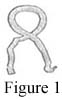
\includegraphics[scale=0.75]{Pym_1}
\end{center}

This figure (see figure 1) gives the general outlines of the chasm, without
the minor cavities in the sides, of which there were several, each cavity having
a corresponding protuberance opposite. The bottom of the gulf was covered to the
depth of three or four inches with a powder almost impalpable, beneath which we
found a continuation of the black granite. To the right, at the lower extremity,
will be noticed the appearance of a small opening; this is the fissure alluded
to above, and to examine which more minutely than before was the object of our
second visit. We now pushed into it with vigor, cutting away a quantity of
brambles which impeded us, and removing a vast heap of sharp flints somewhat
resembling arrowheads in shape. We were encouraged to persevere, however, by
perceiving some little light proceeding from the farther end. We at length
squeezed our way for about thirty feet, and found that the aperture was a low
and regularly formed arch, having a bottom of the same impalpable powder as that
in the main chasm. A strong light now broke upon us, and, turning a short bend,
we found ourselves in another lofty chamber, similar to the one we had left in
every respect but longitudinal form. Its general figure is here given. (See
figure 2.) 
\begin{center}
    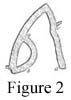
\includegraphics[scale=0.75]{Pym_2}
\end{center}

The total length of this chasm, commencing at the opening \emph{a} and
proceeding round the curve \emph{b} to the extremity \emph{d}, is five hundred
and fifty yards. At \emph{c} we discovered a small aperture similar to the one
through which we had issued from the other chasm, and this was choked up in the
same manner with brambles and a quantity of the white arrowhead flints. We
forced our way through it, finding it about forty feet long, and emerged into a
third chasm. This, too, was precisely like the first, except in its longitudinal
shape, which was thus. (See figure 3.) 
\begin{center}
    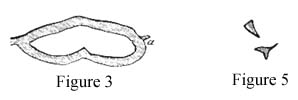
\includegraphics[scale=0.75]{Pym_3-5}
\end{center}


We found the entire length of the third chasm three hundred and twenty yards.
At the point \emph{a} was an opening about six feet wide, and extending fifteen
feet into the rock, where it terminated in a bed of marl, there being no other
chasm beyond, as we had expected. We were about leaving this fissure, into which
very little light was admitted, when Peters called my attention to a range of
singular-looking indentures in the surface of the marl forming the termination
of the \emph{cul-de-sac}. With a very slight exertion of the imagination, the
left, or most northern of these indentures might have been taken for the
intentional, although rude, representation of a human figure standing erect,
with outstretched arm. The rest of them bore also some little resemblance to
alphabetical characters, and Peters was willing, at all events, to adopt the
idle opinion that they were really such. I convinced him of his error, finally,
by directing his attention to the floor of the fissure, where, among the powder,
we picked up, piece by piece, several large flakes of the marl, which had
evidently been broken off by some convulsion from the surface where the
indentures were found, and which had projecting points exactly fitting the
indentures; thus proving them to have been the work of nature. Figure 4 presents
an accurate copy of the whole. 
\begin{center}
    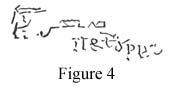
\includegraphics[scale=0.75]{Pym_4}
\end{center}

After satisfying ourselves that these singular caverns afforded us no means
of escape from our prison, we made our way back, dejected and dispirited, to the
summit of the hill. Nothing worth mentioning occurred during the next
twenty-four hours, except that, in examining the ground to the eastward of the
third chasm, we found two triangular holes of great depth, and also with black
granite sides. Into these holes we did not think it worth while to attempt
descending, as they had the appearance of mere natural wells, without outlet.
They were each about twenty yards in circumference, and their shape, as well as
relative position in regard to the third chasm, is shown in figure 5. 

\section{Chapter 24}
On the twentieth of the month, finding it altogether impossible to subsist
any longer upon the filberts, the use of which occasioned us the most
excruciating torment, we resolved to make a desperate attempt at descending the
southern declivity of the hill. The face of the precipice was here of the
softest species of soapstone, although nearly perpendicular throughout its whole
extent (a depth of a hundred and fifty feet at the least), and in many places
even overarching. After a long search we discovered a narrow ledge about twenty
feet below the brink of the gulf; upon this Peters contrived to leap, with what
assistance I could render him by means of our pocket-handkerchiefs tied
together. With somewhat more difficulty I also got down; and we then saw the
possibility of descending the whole way by the process in which we had clambered
up from the chasm when we had been buried by the fall of the hill-that is, by
cutting steps in the face of the soapstone with our knives. The extreme hazard
of the attempt can scarcely be conceived; but, as there was no other resource,
we determined to undertake it. 

Upon the ledge where we stood there grew some filbert-bushes; and to one of
these we made fast an end of our rope of handkerchiefs. The other end being tied
round Peters' waist, I lowered him down over the edge of the precipice until the
handkerchiefs were stretched tight. He now proceeded to dig a deep hole in the
soapstone (as far in as eight or ten inches), sloping away the rock above to the
height of a foot, or thereabout, so as to allow of his driving, with the butt of
a pistol, a tolerably strong peg into the levelled surface. I then drew him up
for about four feet, when he made a hole similar to the one below, driving in a
peg as before, and having thus a resting-place for both feet and hands. I now
unfastened the handkerchiefs from the bush, throwing him the end, which he tied
to the peg in the uppermost hole , letting himself down gently to a station
about three feet lower than he had yet been that is, to the full extent of the
handkerchiefs. Here he dug another hole, and drove another peg. He then drew
himself up, so as to rest his feet in the hole just cut, taking hold with his
hands upon the peg in the one above. It was now necessary to untie the
handkerchiefs from the topmost peg, with the view of fastening them to the
second; and here he found that an error had been committed in cutting the holes
at so great a distance apart. However, after one or two unsuccessful and
dangerous attempts at reaching the knot (having to hold on with his left hand
while he labored to undo the fastening with his right), he at length cut the
string, leaving six inches of it affixed to the peg. Tying the handkerchiefs now
to the second peg, he descended to a station below the third, taking care not to
go too far down. By these means (means which I should never have conceived of
myself, and for which we were indebted altogether to Peters' ingenuity and
resolution) my companion finally succeeded, with the occasional aid of
projections in the cliff, in reaching the bottom without accident. 

It was some time before I could summon sufficient resolution to follow him;
but I did at length attempt it. Peters had taken off his shirt before
descending, and this, with my own, formed the rope necessary for the adventure.
After throwing down the musket found in the chasm, I fastened this rope to the
bushes, and let myself down rapidly, striving, by the vigor of my movements, to
banish the trepidation which I could overcome in no other manner. This answered
sufficiently well for the first four or five steps; but presently I found my
imagination growing terribly excited by thoughts of the vast depths yet to be
descended, and the precarious nature of the pegs and soapstone holes which were
my only support. It was in vain I endeavored to banish these reflections, and to
keep my eyes steadily bent upon the flat surface of the cliff before me. The
more earnestly I struggled \emph{not to think}, the more intensely vivid became
my conceptions, and the more horribly distinct. At length arrived that crisis of
fancy, so fearful in all similar cases, the crisis in which we began to
anticipate the feelings with which we \emph{shall} fall---to picture to
ourselves the sickness, and dizziness, and the last struggle, and the half
swoon, and the final bitterness of the rushing and headlong descent. And now I
found these fancies creating their own realities, and all imagined horrors
crowding upon me in fact. I felt my knees strike violently together, while my
fingers were gradually but certainly relaxing their grasp. There was a ringing
in my ears, and I said, ``This is my knell of death!'' And now I was consumed with
the irrepressible desire of looking below. I could not, I would not, confine my
glances to the cliff; and, with a wild, indefinable emotion, half of horror,
half of a relieved oppression, I threw my vision far down into the abyss. For
one moment my fingers clutched convulsively upon their hold, while, with the
movement, the faintest possible idea of ultimate escape wandered, like a shadow,
through my mind -in the next my whole soul was pervaded with \emph{a longing to
fall}; a desire, a yearning, a passion utterly uncontrollable. I let go at
once my grasp upon the peg, and, turning half round from the precipice, remained
tottering for an instant against its naked face. But now there came a spinning
of the brain; a shrill-sounding and phantom voice screamed within my ears; a
dusky, fiendish, and filmy figure stood immediately beneath me; and, sighing, I
sunk down with a bursting heart, and plunged within its arms. 

I had swooned, and Peters had caught me as I fell. He had observed my
proceedings from his station at the bottom of the cliff; and perceiving my
imminent danger, had endeavored to inspire me with courage by every suggestion
he could devise; although my confusion of mind had been so great as to prevent
my hearing what he said, or being conscious that he had even spoken to me at
all. At length, seeing me totter, he hastened to ascend to my rescue, and
arrived just in time for my preservation. Had I fallen with my full weight, the
rope of linen would inevitably have snapped, and I should have been precipitated
into the abyss; as it was, he contrived to let me down gently, so as to remain
suspended without danger until animation returned. This was in about fifteen
minutes. On recovery, my trepidation had entirely vanished; I felt a new being,
and, with some little further aid from my companion, reached the bottom also in
safety. 

We now found ourselves not far from the ravine which had proved the tomb of
our friends, and to the southward of the spot where the hill had fallen. The
place was one of singular wildness, and its aspect brought to my mind the
descriptions given by travellers of those dreary regions marking the site of
degraded Babylon. Not to speak of the ruins of the disrupted cliff, which formed
a chaotic barrier in the vista to the northward, the surface of the ground in
every other direction was strewn with huge tumuli, apparently the wreck of some
gigantic structures of art; although, in detail, no semblance of art could be
detected. Scoria were abundant, and large shapeless blocks of the black granite,
intermingled with others of marl,\footnote{
The marl was also black; indeed, we noticed no light-coloured substances of any 
kind upon the island.}
and both granulated with metal. Of
vegetation there were no traces whatsoever throughout the whole of the desolate
area within sight. Several immense scorpions were seen, and various reptiles not
elsewhere to be found in the high latitudes. As food was our most immediate
object, we resolved to make our way to the seacoast, distant not more than half
a mile, with a view of catching turtle, several of which we had observed from
our place of concealment on the hill. We had proceeded some hundred yards,
threading our route cautiously between the huge rocks and tumuli, when, upon
turning a corner, five savages sprung upon us from a small cavern, felling
Peters to the ground with a blow from a club. As he fell the whole party rushed
upon him to secure their victim, leaving me time to recover from my
astonishment. T still had the musket, but the barrel had received so much injury
in being thrown from the precipice that T cast it aside as useless, preferring
to trust my pistols, which had been carefully preserved in order. With these I
advanced upon the assailants, firing one after the other in quick succession.
Two savages fell, and one, who was in the act of thrusting a spear into Peters,
sprung to his feet without accomplishing his purpose. My companion being thus
released, we had no further difficulty. He had his pistols also, but prudently
declined using them, confiding in his great personal strength, which far
exceeded that of any person I have ever known. Seizing a club from one of the
savages who had fallen, he dashed out the brains of the three who remained,
killing each instantaneously with a single blow of the weapon, and leaving us
completely masters of the field. 

So rapidly bad these events passed, that we could scarcely believe in their
reality, and were standing over the bodies of the dead in a species of stupid
contemplation, when we were brought to recollection by the sound of shouts in
the distance, It was clear that the savages had been alarmed by the firing, and
that we had little chance of avoiding discovery. To regain the cliff, it would
be necessary to proceed in the direction of the shouts, and even should we
succeed in arriving at its base, we should never be able to ascend it without
being seen. Our situation was one of the greatest peril, and we were hesitating
in which path to commence a flight, when one of the savages whom I bad shot, and
supposed dead, sprang briskly to his feet, and attempted to make his escape. We
overtook him, however, before he had advanced many paces, and were about to put
him to death, when Peters suggested that we might derive some benefit from
forcing him to accompany us in our attempt to escape. We therefore dragged him
with us, making him understand that we would shoot him if he offered resistance.
In a few minutes he was perfectly submissive, and ran by our sides as we pushed
in among the rocks, making for the seashore. 

So far, the irregularities of the ground we had been traversing hid the sea,
except at intervals, from our sight, and, when we first had it fairly in view,
it was perhaps two hundred yards distant. As we emerged into the open beach we
saw, to our great dismay, an immense crowd of the natives pouring from the
village, and from all visible quarters of the island, making toward us with
gesticulations of extreme fury, and howling like wild beasts. We were upon the
point of turning upon our steps, and trying to secure a retreat among the
fastnesses of the rougher ground, when I discovered the bows of two canoes
projecting from behind a large rock which ran out into the water. Toward these
we now ran with all speed, and, reaching them, found them unguarded, and without
any other freight than three of the large Gallipago turtles and the usual supply
of paddles for sixty rowers. We instantly took possession of one of them, and,
forcing our captive on board, pushed out to sea with all the strength we could
command. 

We had not made, however, more than fifty yards from the shore before we
became sufficiently calm to perceive the great oversight of which we had been
guilty in leaving the other canoe in the power of the savages, who, by this
time, were not more than twice as far from the beach as ourselves, and were
rapidly advancing to the pursuit. No time was now to be lost. Our hope was, at
best, a forlorn one, but we had none other. It was very doubtful whether, with
the utmost exertion, we could get back in time to anticipate them in taking
possession of the canoe; but yet there was a chance that we could. We might save
ourselves if we succeeded, while not to make the attempt was to resign ourselves
to inevitable butchery. 

The canoe was modelled with the bow and stern alike, and, in place of turning
it around, we merely changed our position in paddling. As soon as the savages
perceived this they redoubled their yells, as well as their speed, and
approached with inconceivable rapidity. We pulled, however, with all the energy
of desperation, and arrived at the contested point before more than one of the
natives had attained it. This man paid dearly for his superior agility, Peters
shooting him through the head with a pistol as he approached the shore. The
foremost among the rest of his party were probably some twenty or thirty paces
distant as we seized upon the canoe. We at first endeavored to pull her into the
deep water, beyond the reach of the savages, but, finding her too firmly
aground, and there being no time to spare, Peters, with one or two heavy strokes
from the butt of the musket, succeeded in dashing out a large portion of the bow
and of one side. We then pushed off. Two of the natives by this time had got
hold of our boat, obstinately refusing to let go, until we were forced to
despatch them with our knives. We were now clear off, and making great way out
to sea. The main body of the savages, upon reaching the broken canoe, set up the
most tremendous yell of rage and disappointment conceivable. In truth, from
everything I could see of these wretches, they appeared to be the most wicked,
hypocritical, vindictive, bloodthirsty, and altogether fiendish race of men upon
the face of the globe. It is clear we should have had no mercy had we fallen
into their hands. They made a mad attempt at following us in the fractured
canoe, but, finding it useless, again vented their rage in a series of hideous
vociferations, and rushed up into the hills. 

We were thus relieved from immediate danger, but our situation was still
sufficiently gloomy. We knew that four canoes of the kind we had were at one
time in the possession of the savages, and were not aware of the fact (afterward
ascertained from our captive) that two of these had been blown to pieces in the
explosion of the Jane Guy. We calculated, therefore, upon being yet pursued, as
soon as our enemies could get round to the bay (distant about three miles) where
the boats were usually laid up. Fearing this, we made every exertion to leave
the island behind us, and went rapidly through the water, forcing the prisoner
to take a paddle. In about half an hour, when we had gained probably five or six
miles to the southward, a large fleet of the flat-bottomed canoes or rafts were
seen to emerge from the bay evidently with the design of pursuit. Presently they
put back, despairing to overtake us. 


\section{Chapter 25}
We now found ourselves in the wide and desolate Antarctic Ocean, in a
latitude exceeding eighty-four degrees, in a frail canoe, and with no provision
but the three turtles. The long polar winter, too, could not be considered as
far distant, and it became necessary that we should deliberate well upon the
course to be pursued. There were six or seven islands in sight belonging to the
same group, and distant from each other about five or six leagues; but upon
neither of these had we any intention to venture. In coming from the northward
in the Jane Guy we bad been gradually leaving behind us the severest regions of
ice---this, however little it maybe in accordance with the generally received
notions respecting the Antarctic, was a fact---experience would not permit us to
deny. To attempt, therefore, getting back would be folly---especially at so late
a period of the season. Only one course seemed to be left open for hope. We
resolved to steer boldly to the southward, where there was at least a
probability of discovering other lands, and more than a probability of finding a
still milder climate. 

So far we had found the Antarctic, like the Arctic Ocean, peculiarly free
from violent storms or immoderately rough water; but our canoe was, at best, of
frail structure, although large, and we set busily to work with a view of
rendering her as safe as the limited means in our possession would admit. The
body of the boat was of no better material than bark -the bark of a tree
unknown. The ribs were of a tough osier, well adapted to the purpose for which
it was used. We had fifty feet room from stem to stern, from four to six in
breadth, and in depth throughout four feet and a half-the boats thus differing
vastly in shape from those of any other inhabitants of the Southern Ocean with
whom civilized nations are acquainted. We never did believe them the workmanship
of the ignorant islanders who owned them; and some days after this period
discovered, by questioning our captive, that they were in fact made by the
natives of a group to the southwest of the country where we found them,, having
fallen accidentally into the hands of our barbarians. What we could do for the
security of our boat was very little indeed. Several wide rents were discovered
near both ends, and these we contrived to patch up with pieces of woollen
jacket. With the help of the superfluous paddles, of which there were a great
many, we erected a kind of framework about the bow, so as to break the force of
any seas which might threaten to fill us in that quarter. We also set up two
paddle-blades for masts, placing them opposite each other, one by each gunwale,
thus saving the necessity of a yard. To these masts we attached a sail made of
our shirts-doing this with some difficulty, as here we could get no assistance
from our prisoner whatever, although he bad been willing enough to labor in all
the other operations. The sight of the linen seemed to affect him in a very
singular manner. He could not be prevailed upon to touch it or go near it,
shuddering when we attempted to force him, and shrieking out,
``\emph{Tekeli-li!}'' 

Having completed our arrangements in regard to the security of the canoe, we
now set sail to the south-southeast for the present, with the view of weathering
the most southerly of the group in sight. This being done, we turned the bow
full to the southward. The weather could by no means be considered disagreeable.
We had a prevailing andvery gentle wind from the northward, a smooth sea, and
continual daylight. No ice whatever was to be seen; \emph{nor did I ever see one
particle of this after leaving the parallel of Bennet's Islet}. Indeed, the
temperature of the water was here far too warm for its existence in any
quantity. Having killed the largest of our tortoises, and obtained from him not
only food but a copious supply of water, we continued on our course, without any
incident of moment, for perhaps seven or eight days, during which period we must
have proceeded a vast distance to the southward, as the wind blew constantly
with us, and a very strong current set continually in the direction we were
pursuing. 

\emph{March} 1st.\footnote{For obvious
reasons I cannot pretend to strict accuracy in these dates. They are given
principally with a view to perspicuity of narration, and as set down in my
pencil memorandum.} 
Many unusual phenomena now -indicated
that we were entering upon a region of novelty and wonder. A high range of light
gray vapor appeared constantly in the southern horizon, flaring up occasionally
in lofty streaks, now darting from cast to west, now from west to east, and
again presenting a level and uniform summit-in short, having all the wild
variations of the Aurora Borealis. The average height of this vapor, as apparent
from our station, was about twenty-five degrees. The temperature of the sea
seemed to be increasing momentarily, and there was a very perceptible alteration
in its color. 

\emph{March} 2d. To-day by repeated questioning of our captive, we came to
the knowledge of many particulars in regard to the island of the massacre, its
inhabitants, and customs-but with these how can I \emph{now} detain the reader?
I may say, however, that we learned there were eight islands in the group-that
they were governed by a common king, named \emph{Tsalemon} or \emph{Psalemoun},
who resided in one of the smallest of the islands; that the black skins forming
the dress of the warriors came from an animal of huge size to be found only in a
valley near the court of the king-that the inhabitants of the group fabricated
no other boats than the flat-bottomed rafts; the four canoes being all of the
kind in their possession, and, these having been obtained, by mere accident,
from some large island in' the southwest---that his own name was Nu-Nu-that he
had no knowledge of Bennet's Islet---and that the appellation of the island he
had left was \emph{Tsalal}. The commencement of the words \emph{Tsalemon} and
\emph{Tsalal} was given with a prolonged hissing sound, which 'we found it
impossible to imitate, even after repeated endeavors, and which was precisely
the same with the note of the black bittern we had eaten up on the summit of the
hill. 

\emph{March} 3d. The heat of the water was now truly remarkable, and in color
was undergoing a rapid change, being no longer transparent, but of a milky
consistency and hue. In our immediate vicinity it was usually smooth, never so
rough as to endanger the canoe---but we were frequently surprised at perceiving,
to our right and left, at different distances, sudden and extensive agitations
of the surface these, we at length noticed, were always preceded by wild
flickerings in the region of vapor to the southward. 

\emph{March} 4th. To-day, with the view of widening our sail, the breeze from
the northward dying away perceptibly, I took from my coat-pocket a white
handkerchief. Nu-Nu was seated at my elbow, and the linen accidentally flaring
in his face, he became violently affected with convulsions. These were succeeded
by drowsiness and stupor, and low murmurings of ``\emph{Tekeli-li!
Tekeli-li!}'' 

\emph{March} 5th. The wind had entirely ceased, but it was evident that we
were still hurrying on to the southward, under the influence of a powerful
current. And now, -indeed, it would seem reasonable that we should experience
some alarm at the turn events were taking-but we felt none. The countenance of
Peters indicated nothing of this nature, although it wore at times an expression
I could not fathom. The polar winter appeared to be coming on---but coming
without its terrors. I felt a \emph{numbness} of body and mind-a dreaminess of
sensation but this was all. 

\emph{March} 6th. The gray vapor had now arisen many more degrees above the
horizon, and was gradually losing its grayness of tint. The heat of the water
was extreme, even unpleasant to the touch, and its milky hue was more evident
than ever. Today a violent agitation of the water occurred very close to the
canoe. It was attended, as usual, with a wild flaring up of the vapor at its
summit, and a momentary division at its base. A fine white powder, resembling
ashes-but certainly not such-fell over the canoe and over a large surface of the
water, as the flickering died away among the vapor and the commotion subsided in
the sea. Nu-Nu now threw himself on his face in the bottom of the boat, and no
persuasions could induce him to arise. 

\emph{March} 7th. This day we questioned Nu-Nu concerning the motives of his
countrymen in destroying our companions; but he appeared to be too utterly
overcome by terror to afford us any rational reply. He still obstinately lay in
the bottom of the boat; and, upon reiterating the questions as to the motive,
made use only of idiotic gesticulations, such as raising with his forefinger the
upper lip, and displaying the teeth which lay beneath it. These were black. We
had never before seen the teeth of an inhabitant of Tsalal. 

\emph{March} 8th. To-day there floated by us one of the white animals whose
appearance upon the beach at Tsalal had occasioned so wild a commotion among the
savages. I would have picked it up, but there came over me a sudden
listlessness, and I forbore. The heat of the water still increased, and the hand
could no longer be endured within it. Peters spoke little, and I knew not what
to think of his apathy. Nu-Nu breathed, and no more. 

\emph{March} 9th. The whole ashy material fell now continually around us, and
in vast quantities. The range of vapor to the southward had arisen prodigiously
in the horizon, and began to assume more distinctness of form. I can liken it to
nothing but a limitless cataract, rolling silently into the sea from some
immense and far-distant rampart in the heaven. The gigantic curtain ranged along
the whole extent of the southern horizon. It emitted no sound. 

\emph{March} 21st. A sullen darkness now hovered above us-but from out the
milky depths of the ocean a luminous glare arose, and stole up along the
bulwarks of the boat. We were nearly overwhelmed by the white ashy shower which
settled upon us and upon the canoe, but melted into the water as it fell. The
summit of the cataract was utterly lost in the dimness and the distance. Yet we
were evidently approaching it with a hideous velocity. At intervals there were
visible in it wide, yawning, but momentary rents, and from out these rents,
within which was a chaos of flitting and indistinct images, there came rushing
and mighty. but soundless winds, tearing up the enkindled ocean in their
course. 

\emph{March} 22d. The darkness had materially increased, relieved only by the
glare of the water thrown back from the white curtain before us. Many gigantic
and pallidly white birds flew continuously now from beyond the veil, and their
scream was the eternal \emph{Tekeli-li!} as they retreated from our vision.
Hereupon Nu-Nu stirred in the bottom of the boat; but upon touching him we found
his spirit departed. And now we rushed into the embraces of the cataract, where
a chasm threw itself open to receive us. But there arose in our pathway a
shrouded human figure, very far larger in its proportions than any dweller among
men. And the hue of the skin of the figure was of the perfect whiteness of the
snow. 

\section{Note}
\textuppercase{THE} circumstances connected with the late sudden and distressing death of Mr.
Pym are already well known to the public through the medium of the daily press.
It is feared that the few remaining chapters which were to have completed his
narrative, and which were retained by him, while the above were in type, for the
purpose of revision, have been irrecoverably lost through the accident by which
he perished himself. This, however, may prove not to be the case, and the
papers, if ultimately found, will be given to the public. 

No means have been left untried to remedy the deficiency. The gentleman whose
name is mentioned in the preface, and who, from the statement there made, might
be supposed able to fill the vacuum, has declined the task---this for
satisfactory reasons connected with the general inaccuracy of the details
afforded him, and his disbelief in the entire truth of the latter portions of
the narration. Peters, from whom some information might be expected, is still
alive, and a resident of Illinois, but cannot be met with at present. He may
hereafter be found, and will, no doubt, afford material for a conclusion of Mr.
Pym's account. 

The loss of the two or three final chapters (for there were but two or three)
is the more deeply to be regretted, as, it cannot be doubted, they contained
matter relative to the Pole itself, or at least to regions in its very near
proximity; and as, too, the statements of the author in relation to these
regions may shortly be verified or contradicted by means of the governmental
expedition now preparing for the Southern Ocean. 

On one point in the Narrative some remarks may be well offered; and it would
afford the writer of this appendix much pleasure if what he may here observe
should have a tendency to throw credit, in any degree, upon the very singular
pages now published. We allude to the chasms found in the island of Tsalal, and
%TODO: replaced page reference ("figures upon pages 182, 183, 184, 185") with 
%      chapter reference. Can this be fixed?
%      Similar to: http://xroads.virginia.edu/~MA98/silverman/poe/agp_note.html
to the whole of the figures presented in Chapter~23. 

Mr. Pym has given the figures of the chasm without comment, and speaks
decidedly of the \emph{indentures} found at the extremity of the most easterly
of these chasms as having but a fanciful resemblance to alphabetical characters,
and, in short, as being positively \emph{not such}. This assertion is made in a
manner so simple, and sustained by a species of demonstration so conclusive
(viz., the fitting of the projections of the fragments found among the dust into
the indentures upon the wall), that we are forced to believe the writer in
earnest; and no reasonable reader should suppose otherwise. But as the facts in
relation to \emph{all} the figures are most singular (especially when taken in
connexion with statements made in the body of the narrative), it may be as well
to say a word or two concerning them all---this, too, the more especially as the
facts in question have, beyond doubt, escaped the attention of Mr. Poe. 

Figure 1, then figure 2, figure 3, and figure 5, when conjoined with one
another in the precise order which the chasms themselves presented, and when
deprived of the small lateral branches or arches (which, it will be remembered,
served only as means of communication between the main chambers, and were of
totally distinct character), constitute an Ethiopian verbal root --- the root 
\inlineimage{Pym_Inline_1}
``To be shady''---whence all the inflections of shadow or
darkness. 

In regard to the ``left or most northwardly'' of the indentures in figure 4, it
is more than probable that the opinion of Peters was correct, and that the
hieroglyphical appearance was really the work of art, and intended as the
representation of a human form. The delineation is before the reader, and he
may, or may not, perceive the resemblance suggested; but the rest of the
indentures afford strong confirmation of Peters's idea. The upper range is
evidently the Arabic verbal root 
\inlineimage{Pym_Inline_2}
``To be white,'' whence all the inflections of brilliancy and whiteness. The lower
range is not so immediately perspicuous. The characters are somewhat broken and
disjointed; nevertheless, it cannot be doubted that, in their perfect state,
they formed the full Egyptian word 
\inlineimage{Pym_Inline_3}
``The region of the south.'' It should be observed that these interpretations
confirm the opinion of Peters in regard to the ``most northwardly'' of the
figures. The arm is outstretched towards the south. 

Conclusions such as these open a wide field for speculation and exciting
conjecture. They should be regarded, perhaps, in connexion with some of the most
faintly-detailed incidents of the narrative; although in no visible manner is
this chain of connexion complete. Tekeli-li! was the cry of the affrighted
natives of Tsalal upon discovering the carcass of the \emph{white} animal picked
up at sea. This also was the shuddering exclamation of the captive Tsalalian
upon encountering the \emph{white} materials in possession of Mr. Pym. This also
was the shriek of the swift-flying, \emph{white}, and gigantic birds which
issued from the vapoury \emph{white} curtain of the South. Nothing \emph{white}
was to be found at Tsalal, and nothing otherwise in the subsequent voyage to the
region beyond. It is not impossible that ``Tsalal,'' the appellation of the island
of the chasms, may be found, upon minute philological scrutiny, to betray either
some alliance with the chasms themselves, or some reference to the Ethiopian
characters so mysteriously written in their windings. 

``\emph{I have graven it within the hills, and my vengeance upon the dust within
the rock.}'' 
\bigskip
\begin{center}
    \textuppercase{THE END.}
\end{center}

\end{document}

